\documentclass[oneside]{book}
\usepackage[a4paper, total={6in, 8in}]{geometry}
\usepackage[italian]{babel}
\usepackage[utf8]{inputenc}
\usepackage[T1]{fontenc}
\usepackage{amsmath}
\usepackage{amsfonts}
\usepackage{listings}
\usepackage{hyperref}
\usepackage{siunitx}
\usepackage{fancyhdr}
\pagestyle{fancy}
\usepackage{textcomp}
\usepackage{makecell}
\usepackage[font=small,labelfont=bf]{caption}
\usepackage{pdfpages}
\usepackage{multicol}
\usepackage[ruled,vlined]{algorithm2e}
\usepackage{mhchem}
\usepackage{float}
\usepackage{graphicx}
\pagestyle{fancy}
\fancyhf{}
\lhead{\rightmark}
\cfoot{\leftmark}
\rfoot{\thepage}

\setcounter{secnumdepth}{5}

\lstset{
    frame=tb, % draw a frame at the top and bottom of the code block
    tabsize=4, % tab space width
    showstringspaces=false, % don't mark spaces in strings
    numbers=none, % display line numbers on the left
    commentstyle=\color{green}, % comment color
    keywordstyle=\color{red}, % keyword color
    stringstyle=\color{blue}, % string color
    breaklines=true,
    postbreak=\mbox{\textcolor{green}{$\hookrightarrow$}\space}
}

\renewcommand{\lstlistingname}{}% Listing -> Algorithm
\renewcommand{\lstlistlistingname}{Algoritmi}% List of Listings -> List of Algorithms
\author{
  Giacomo Fantoni \\
  \small Telegram: \href{https://t.me/GiacomoFantoni}{@GiacomoFantoni} \\[3pt]
  Github: \href{https://github.com/giacThePhantom/AlgoritmiStruttureDati}{https://github.com/giacThePhantom/AlgoritmiStruttureDati}}


\renewcommand*{\listalgorithmcfname}{}
\renewcommand*{\algorithmcfname}{}
\renewcommand*{\algorithmautorefname}{}
\renewcommand{\thealgocf}{}


\title{\Huge \textbf{Introduction to machine learning}}

\author{
  Giacomo Fantoni \\
  \small Telegram: \href{https://t.me/GiacomoFantoni}{@GiacomoFantoni} \\[3pt]
  \small Github: \href{https://github.com/giacThePhantom/intro2ml}{https://github.com/giacThePhantom/intro2ml}}
\begin{document}

	\maketitle
	\tableofcontents
	\chapter{Introduzione}

\section{Definizioni}
Si intende per machine learning lo studio di algoritmi che migliorano autonomamente attraverso l'esperienza.
\`E un campo dell'intelligenza artificiale.
Stravolge il paradigma convenzionale della programmazione: un algoritmo di machine learning infatti prende come input un insieme di dati e risultati in modo da produrre un programma che fornisce un risultato appropriato.
Coinvolge pertanto la scoperta automatica di regolarit\`a nei dati attraverso algoritmi in modo da poter compiere azioni basate su di essi.

\section{Processo}
Il machine learning permette ai computer di acquisire conoscenza attraverso algoritmi che inferiscono e imparano da dati.
Questa conoscenza viene rappresentata da un modello che pu\`o essere utilizzato su nuovi dati.

	\subsection{Il processo di apprendimento}
	Il processo di apprendimento in particolare coinvolge diversi passaggi:
	\begin{multicols}{2}
		\begin{itemize}
			\item Acquisizione dei dati dal mondo reale attraverso dispositivi di misurazione come sensori o database.
			\item Preprocessamento dei dati: filtraggio del rumore, estrazione delle feature e normalizzazione.
			\item Riduzione dimensionale: selezione e proiezione delle feature.
			\item Apprendimento del modello: classificazione, regressione, clustering e descrizione.
			\item Test del modello: cross-validation e bootstrap.
			\item Analisi dei risultati.
		\end{itemize}
	\end{multicols}

\section{Modello}
Un algoritmo di machine learning impara dall'esperienza $E$ in rispetto di una classe di compiti $T$ e di misurazione delle performance $P$, se la $P$ di $T$ aumenta con $E$.
Si nota pertanto come un compito di machine learning ben definito possiede una tripla:
$$<T, P, E>$$
Andiamo a vedere degli esempi:
\begin{itemize}
	\item T: Categorizzazzione delle email come spam, P: Percentuale delle email categorizzate correttamente, E: Database delle parole email, alcune etichettate da umani
\end{itemize}
\section{Deep learning}
Il deep learning \`e un sottoinsieme del machine learning che permette a modelli computazionali composti di multipli strati di imparare la rappresentazione di dati con multipli livelli di astrazione.
Si utilizza pertanto una rete neurale con diversi strati di nodi tra input e output.
Questa serie di strati tra input e output computa caratteristiche rilevanti automaticamente in una serie di passaggi.
Questi algoritmi sono resi possibili da:
\begin{multicols}{2}
	\begin{itemize}
		\item Enorme mole di dati disponibili.
		\item Aumento del potere computazionale.
		\item Aumento del numero di algoritmi di machine learning e della teoria sviluppata dai ricercatori.
		\item Aumento del supporto dall'industria.
	\end{itemize}
\end{multicols}

	\chapter{Machine learning basics}

\section{Introduzione}
Il machine learning permette ai computer di acquisire conoscenza attraverso algoritmi che imparano e inferiscono dai dati.
Tale conoscenza viene rappresentata da un modello che viene poi utilizzato su dati futuri.

	\subsection{Processo di learning}
	Si individua un processo di learning:
	\begin{multicols}{2}
		\begin{itemize}
			\item Acquisizione di dati dal mondo reale attraverso sensori.
			\item Preprocessamento dei dati: eliminazione del rumore, estrazione delle features e normalizzazione.
			\item Riduzione di dimensionalit\`a attraverso selezione e proiezione di features.
			\item Learning del modello: classification, regression, clustering e description.
			\item Test del modello attraverso cross-validation e bootstrap.
			\item Analisi dei risultati.
		\end{itemize}
	\end{multicols}

\section{Dati}
I dati disponibili ad un algoritmo di machine learning sono tipicamente un insieme di esempi.
Questi esempi sono tipicamente rappresentati come un array di features, caratteristiche dei dati di interesse per lo studio in atto.

	\subsection{Training e test set}
	In particolare per questi algoritmi si assume sempre che il training e il test set siano distribuiti secondo variabili indipendenti e identicamente distribuite (\emph{i.i.d})
	La distribuzione $P_{data}$ \`e tipicamente sconosciuta ma si pu\`o campionare, attraverso un modello probabilistico di learning.
	In particolare la distribuzione di probabilit\`a di coppie di esempio e label viene detta data generating distribution e sia il training data che il test set sono generati basandosi su di essa.

\section{Task}
Si intende per task una rappresentazione del tipo di predizione che viene svolta per risolvere un problema su dei dati.
Viene identificata con un insieme di funzioni che possono potenzialmente risolverla.
In generale consiste di una funzione che assegna ogni input $x\in\mathcal{X}$ a un output $y\in\mathcal{Y}$:
$$f:\mathcal{X}\rightarrow\mathcal{Y}\qquad\mathcal{F}_{task}\subset\mathcal{Y^X}$$
La natura di $\mathcal{X},\mathcal{Y}, \mathcal{F}_{task}$ dipende dal tipo di task.

\section{Modello}
Un modello \`e un programma per risolvere un problema.
\`E cio\`e l'implementazione di una funzione $f\in\mathcal{F}_{task}$ che pu\`o essere computata.
Un insieme di modelli formano uno spazio di ipotesi:
$$\mathcal{H}\subset\mathcal{F}_{task}$$
L'algoritmo cerca una soluzione nello spazio di ipotesi.
Esistono diversi tipi di modello:
\begin{multicols}{2}
	\begin{itemize}
		\item Generativi e discriminativi.
		\item Parametrici e non parametrici.
	\end{itemize}
\end{multicols}

	\subsection{Target ideale}
	Il target ideale del modello \`e quello di minimizzare una funzione di errore (generalizzazione)
	$$E(f;P_{data})$$
	Questa funzione determina quanto bene una soluzione $f\in\mathcal{F}_{task}$ fitta dei dati.
	Guida pertanto la selezione della migliore soluzione in $\mathcal{F}_{task}$.
	Pertanto:
	$$f^*\in arg\min\limits_{f\in\mathcal{F}_{task}}E(f;P_{data})$$

	\subsection{Target feasible}
	Si deve restringere il focus sul trovare funzioni che possono essere implementate e valutate in maniera trattabile.
	Si definisce pertanto uno spazio di ipotesi del modello $\mathcal{H}\subset\mathcal{F}_{task}$ e si cerca la soluzione all'interno di quello spazio:
	$$f^*_{\mathcal{H}}\in arg\min\limits_{f\in\mathcal{H}} E(f;P_{data})$$
	Si noti come questa funzione non possa essere computata correttamente in quanto $P_{data}$ \`e sconosciuta.

	\subsection{Target attuale}
	Per trovare il target attuale si deve lavorare su un campione di dati o il training set
	$$\mathcal{D}_n=\{z_1,\dots,z_n\}$$
	Dove
	$$z_i=(x_i,y_i)\in\mathcal{X}\times\mathcal{Y}$$
	$$z_i\sim P_{data}$$
	Pertanto in:
	$$f^*_{\mathcal{H}}\in arg\min\limits_{f\in\mathcal{H}} E(f;P_{data})$$
	$E(f;P_{data})$ \`e il training error.

	\subsection{Funzione di errore}
	Le funzioni di generalizzazione e di training error possono essere scritte in termini di una pointwise loss $l(f;z)$ che misura l'errore che avviene a $f$ su un esempio di training $z$.
	$$E(f;P_{data})=\mathbb{E}_{z\sim P_{data}}[l(f;z)]$$
	$$E(f;\mathcal{D}_n)=\dfrac{1}{n}\sum\limits_{i=1}^nl(f;z_i)$$
	Si nota pertanto come l'algoritmo di learning risolve il problema di ottimizzazione con target:
	$$f^*_\mathcal{H}(\mathcal{D}_n)$$

	\subsection{Tipi di errore}
	\begin{multicols}{2}
		\begin{itemize}
			\item Underfitting il modello non fitta sui dati di training, avviene per mancanza di dati.
			\item Overfitting quando i training data sono rumorosi e il modello li fitta perfettamente, ma impara un modello che si adatta solo su di essi e non fitta dati dal mondo reale.
			\item Estimation error, indotto imparando da un campione di dati.
			\item Approximation error, indotto dallo spazio di ipotesi $\mathcal{H}$.
			\item Irreducible error a causa della variabilit\`a intrinseca.
		\end{itemize}
	\end{multicols}

	\subsection{Stimare l'errore di generalizzazione}
	L'errore di generalizzazione pu\`o essere stimato utilizzando diversi insiemi di training, validation e test.
	Si usa il training set per fare training di un modello, quello di validazione per valutarlo e sistemare i suoi iperparametri e dopo di quello si sceglie il modello migliore che si misura attraverso le performance sul test set.

		\subsubsection{Migliorare la generalizzazione}
		La generalizzazione pu\`o essere migliorata:
		\begin{multicols}{2}
			\begin{itemize}
				\item Evitando di ottenere il minimo sul training error.
				\item Riducendo la capacit\`a del modello.
				\item Cambiando l'obiettivo con un termine di regolarizzazione.
				\item Iniettando rumore nell'algoritmo.
				\item Fermando l'algoritmo prima che converga.
				\item Aumentantdo la quantit\`a di dati.
				\item Aggiungendo pi\`u campioni di training.
				\item Aumentando il training set con trasformazioni.
				\item Combinando predizioni da pi\`u modelli decorrelati o ensembling.
			\end{itemize}
		\end{multicols}

			\paragraph{Regolarizzazione}
			Si intende per regolarizzazione la modifica della funzione di training error con un termine $\Omega(f)$ che penalizza soluzioni complesse:
			$$E_{reg}(f;\mathcal{D}_n)=E(f;\mathcal{D}_n)+\lambda_n\Omega(f)$$


\section{Tipi di learning}

	\subsection{Supervised learning}
	Nel supervised learning vengono dati in input a un modello o predittore un insieme di esempi che possiedono una label.
	Il modello poi impara a creare delle predizioni su un nuovo esempio.

		\subsubsection{Dati}
		Nel caso del supervised learning i dati creano una distribuzione:
		$$p_{data}\in\Delta(\mathcal{X}\times\mathcal{Y})$$

		\subsubsection{Classificazione}
		In un problema di classificazione si trova un insieme finito di label discrete.
		In particolare dato un training set $\mathcal{T} = \{(x_1, u_1),\dots(x_m, y_m)\}$, si deve imparare una funzione $f$ per predirre $y$ dato $x$.
		$f$ sar\`a pertanto:
		$$f:\mathbb{R}^d \rightarrow\{1, 2, \dots, k\}$$
		Dove $d$ \`e la dimensionalit\`a di $x$ e $k$ il numero di labels distinte.

			\paragraph{Task}
			Si deve pertanto trovare una funzione $f\in\mathcal{Y^X}$ che assegna ogni input $x\in\mathcal{X}$ a una label discreta.
			$$f(x)\in\mathcal{Y}=\{c_1,\dots,c_k\}$$

		\subsubsection{Regression}
		Un problema di regressione presenta un insieme di label continue.
		Dato un training set $\mathcal{T}=\{(x_1, y_1),\dots,(x_m,y_m)\}$, si deve imparare una funzione $f$ per predirre $y$ dato $x$.
		$f$ sar\`a pertanto:
		$$f:\mathbb{R}^d\rightarrow\mathbb{R}$$
		Dove $d$ \`e la dimensionalit\`a di $x$.

			\paragraph{Task}
			Si deve trovare una funzione $f(x)\in\mathcal{Y}$ che assegna ogni input a una label continua.

		\subsubsection{Ranking}
		Il ranking \`e un tipo particolare di classificazione in cui una label \`e un ranking.

	\subsection{Unsupervised learning}
	Nel unsupervised learning vengono dati in input a un modello o predittore un insieme di esempi senza label.
	Il modello impara a creare delle predizioni su un nuovo esempio.

		\subsubsection{Dati}
		Nel caso del supervised learning i dati creano una distribuzione:
		$$p_{data}\in\Delta(\mathcal{X})$$

		\subsubsection{Clustering}
		Nel clustering, data $\mathcal{T}=\{x_1, \dots, x_m\}$ si deve trovare la struttura nascosta che intercorre tra le $x$ o i clusters.

			\paragraph{Task}
			Si deve trovare una funzione $f\in\mathbb{N}^{\mathcal{X}}$ che assegna ogni input $x\in\mathcal{X}$ a un indice di cluster $f(x)\in\mathbb{N}$.
			Tutti i punti mappati sullo stesso indice formano un cluster.

		\subsubsection{Dimensionality reduction}
		Nella dimensionality reduction si tenta di ridurre il numero di variabili sotto considerazione ottenendo un insieme di variabili principali.

			\paragraph{Task}
			Si deve trovare una funzione $f\in\mathcal{Y}^\mathcal{X}$ che mappa ogni input di molte dimensioni $x\in\mathcal{X}$ a un output a dimensione minore $f(x)\in\mathcal{Y}$, dove $dim(\mathcal{Y})\ll dim(\mathcal{X})$

	\subsection{Reinforcement learning}
	Nel reinforcement learning un agente impara dall'ambiente interagendo con esso e ricevendo premi per lo svolgimento di azioni particolari.
	In particolare, data una sequenza di esempi o stati e una reward dopo il completamento di tale sequenza si impara a predirre l'azione da svolgere per uno stato o esempio individuale.

\section{Polynomial curve fitting}

	\subsection{Dati}
	L'insieme dei dati $\mathcal{D}_n$ consiste di coppie:
	$$\mathcal{D}_n = \{(x_1, y_1),\dots,(x_n,y_n)\}$$
	I dati sono generati dalla funzione $\sin(2\pi x)$ con del rumore.
	Il training set consiste di $10$ punti: $n = 10$.

	\subsection{Modello e spazio di ipotesi}
	Il modello per il polynomial curve fitting \`e:
	$$f_w(x) = \sum\limits_{j = 0}^M w_jx^j$$
	\`E parametrico, dove i parametri sono $\{w_0,\dots, w_,\}$.
	Lo spazio di ipotesi per $M\in\mathbb{N}$ fissato \`e:
	$$\mathcal{H}_M = \{f_w:w\in\mathbb{R}^M\}$$

	\subsection{Error function}
	La funzione di errore per il polynomial curve fitting consiste della media tra le distanze quadratiche tra la predizione effettuata e l'effettiva label.
	La pointwise loss:
	$$l(f;(x_i,y_i)) = [f(x_i) - y_i]^2$$
	La funzione di errore \`e pertanto:
	$$E(f;\mathcal{D}_n) = \mathbb{E}(l(f;(x_i,y_i))) = \frac{1}{n}\sum\limits_{i=1}^n[f(x_i)-y_i]^2$$

	\subsection{Funzione obiettivo}
	Si ricordi che la funzione obiettivo \`e:
	$$f^*_{\mathcal{H}_M}(\mathcal{D}_n)\in\arg\min\limits_{f\in\mathcal{H}_M}E(f;\mathcal{D}_n)$$
	Equivalente rispetto a $f_{w^*}$ dove:
	$$w^*\in\arg\min\limits_{w\in\mathbb{R}^M}\frac{1}{n}\sum\limits_{i=1}^n[f_w(x_i)-y_i]^2$$
	Si noti come questa richieda la risoluzione di un sistema lineare di equazioni.
	Il cambiamento di $M$ influisce grandemente sull'accuratezza della predizione, andando a determinare casi di overfitting o underfitting.
	Con questo caso particolare si trova la soluzione migliore con $M=3$.

	\subsection{Regolarizzazione}
	Il polynomial curve fitting si regolarizza penalizzando i polinomi con grandi coefficienti:
	$$E_{reg}(f_w;\mathcal{D}_n) = \frac{1}{n}\sum\limits_{i=1}^n[f_w(x_i)-y_i]^2 + \frac{\lambda}{n}||w||^2$$
	Dove $||w||^2 = \sum\limits_{i = 1}^n w_i^2$.

	\chapter{KNN}

\section{Introduzione}
Si possono considerare gli esempi come punti in uno spazio $n$ dimensionale dove $n$ \`e il numero di features.
Per classificare un esempio $d$ si pu\`o mettere a $d$ una label uguale a quella dell'esempio pi\`u vicino a $d$ nel training set.
Questo concetto viene esteso nel $K$-nearest neighbour o \emph{K-NN} in cui per classificare un esempio $d$ si trovano i $k$ esempi pi\`u vicini di $d$ e si sceglie la label in maggior numero tra i $k$ vicini pi\`u prossimi.

\section{Misurare la distanza}
Misurare la distanza tra due esempi \`e specifico al problema, ma un modo possibile \`e la distanza euclidea:
$$D(a,b)=\sqrt{(a_1-b_1)^2+\cdots+(a_n-b_n)^2}$$

\section{Decision boundaries}
I decision boundaries sono posti nello spazio delle features dove la classificazione di un punto o un esempio cambia.
In particolare \emph{K-NN} definisce dei decision boundaries localmente tra le classi.

\section{Il ruolo di $K$}
I fattori che determinano la bont\`a di un algoritmo di machine learning sono la sua abilit\`a di minimizzare il training error e minimizzare il gap tra il training error e il test error.
Questi due fattori corrispondono a underfitting e overfitting.

	\subsection{Underfitting}
	L'underfitting avviene quando il modello non \`e capace di ottenere un valore di errore abbastanza piccolo sul training set.

	\subsection{Overfitting}
	L'overfitting avviene quando il gap tra il training error e il test error \`e troppo grande.

\section{Scelta di $K$}
Il valore di $K$ comprende euristiche comuni come $3, 5, 7$ o un numero dispari per evitare pareggi.
Pu\`o essere scelto utilizzando dati di sviluppo.
Per classificare un esempio $d$ si trovano i $k$ vicini pi\`u prossimi di $d$ e si sceglie la classe pi\`u presente nei $k$ scelti.

\section{Variaizoni di $K$}
Invece di scegliere i $K$ vicini pi\`u prossimi si possono contare tutti gli esempi in una distanza fissata.

	\subsection{\emph{K-NN} pesata}
	Si pu\`o pesare il voto di tutti gli esempi in modo che esempi pi\`u vicini pesino di pi\`u.
	Si usa speso qualche tipo di decadimento esponenziale.

	\chapter{Modelli lineari}

\section{Introduzione}
Alcuni approcci del machine learning fanno delle forti assunzioni riguardo i dati.
Questo avviene in quanto se le assunzioni sono vere si possono raggiungere performance migliori. 
Conoscenza pregressa del dominio ci permette di fare assunzioni sui dati.
In caso contrario l'approccio pu\`o fallire miseramente.
Altri approcci che non fanno molte assunzioni riguardo i dati invece permettono di imparare da dati pi\`u vari ma sono pi\`u proni a overfitting e richiedono pi\`u dati di training.

	\subsection{Bias}
	Il bias di un modello \`e quanto forte le assunzioni del modello sono.
	I classificatori a low-bias fanno delle assunzioni minime riguardo i dati come \emph{k-NN} (che assume unicamente che la vicinanza \`e correlata alla classe) e \emph{DT}, e quindi ci permettono di imparare sempre \emph{qualcosa}.
	I classificatori a high-bias fanno assunzioni forti riguardo ai dati.
	
\section{Linear separability}
L'assunzione strong-bias dei modelli lineari \`e la linear separability, ovvero che in due dimensioni le classi si possano separare attraverso una linea, mentre in dimensioni maggiori da un hyperplane.
Un modello lineare \`e pertanto un modello che assume che i dati sono linearmente separabili. 
	
	\subsection{Definire una linea}
	Ogni coppia di valori $(w_1,w_2)$ definisce una linea attraverso l'origine:
	$$0=w_1f_1+w_2f_2$$
	Si pu\`o inoltre vedere il vettore $\overrightarrow{w}=(w_1, w_2)$ come il vettore dei pesi perpendicolare alla linea.
	Per classificare i punti rispetto alla linea si considera il segno sostituendo i punti a $f_1$ e $f_2$.
	La positivit\`a o negativit\`a indica il lato della linea.
	Avere una linea che attraversa sempre l'origine è limitante, dunque i pu\`o estendere l'equazione con:
	$$a=w_1f_1+w_2f_2$$
	In questo modo la linea interseca l'asse delle $y$ in $a$. \ref{fig:chapter04-00}
	
	\begin{figure}
		\centering
		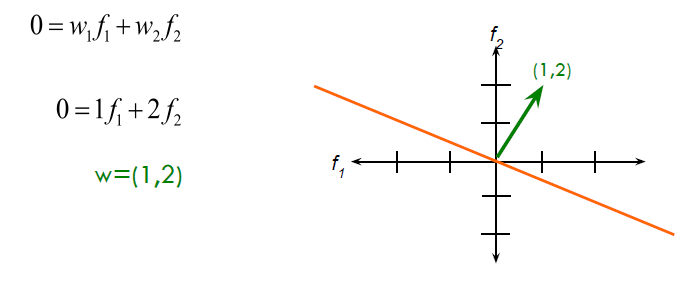
\includegraphics[width=0.6\linewidth]{imgs/chapter4/img0}
		\caption{Definire una linea}
		\label{fig:chapter04-00}
	\end{figure}

\section{Definizione di modello lineare}
Si definisce un modello lineare in uno spazio $n$ dimensionale, dove $n$ \`e il numero di features attraverso $n+1$ pesi.
$$0=b+\sum\limits_{i=1}^nw_if_i$$
In un modello lineare si classifica un nuovo esempio moltiplicandolo con il vettore dei pesi, aggiungendo il bias e controllando il segno del risultato.
Questo determina la classe dell'esempio. 
Siamo dunque interessati alla migliore coppia pesi e bias che separa i dati.

	\subsection{Training}
	Il training di un modello lineare avviene online, ovvero a differenza del modo in batch in cui vengono dati i training data come $\{(x_i, y_i):1\le i\le n\}$, i data points arrivano uno alla volta.
	L'algoritmo allora riceve un esempio $x_i$ senza label, predice la classificazione di questo esempio e confronta la predizione con la risposta corretta $y_i$.
	Infine aggiorna il proprio modello, dunque modifica la linea. 
	Se abbiamo tutti i dati a disposizione possiamo comunque fare training online.
	Le applicazioni del training online sono varie: data streams, dataset di grandi dimensioni, applicazioni che preservano la privacy.
	\subsection{Esempio di training}
	Supponiamo di avere il modello $w=(1,0)$ in figura \ref{fig:chapter04-02}. 
	Abbiamo appena ricevuto un punto in $(-1,1)$, le label ci dicono che quel punto dovrebbe essere classificato come positivo, ma al momento si trova nel lato negativo della linea. 
	Dunque i pesi vanno aggiornati.
	$$w_1*f_1 + w_2 * f_2 = 1 * -1 + 0 * -1 = -1$$
	
	Abbiamo ottenuto un risultato negativo, confermando che i pesi vadano aggiornati, al fine di ottenere un risultato positivo. 
	Possiamo scegliere vari modi per aggiornare i pesi, uno di questi \`e aggiornarli nel seguente modo: $w=(0,1)$, ottenendo il modello in figura \ref{fig:chapter04-03}.
	
	\begin{figure}
		\centering
		\begin{minipage}{.5\textwidth}
			\centering
			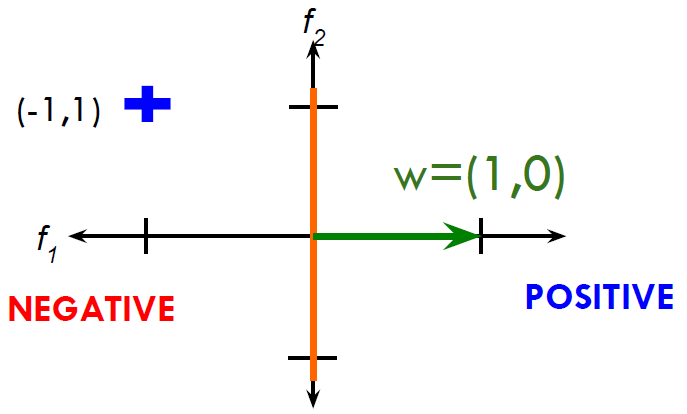
\includegraphics[width=1\linewidth]{imgs/chapter4/img2}
			\caption{Esempio: Modello}
			\label{fig:chapter04-02}
		\end{minipage}%
		\begin{minipage}{.5\textwidth}
			\centering
			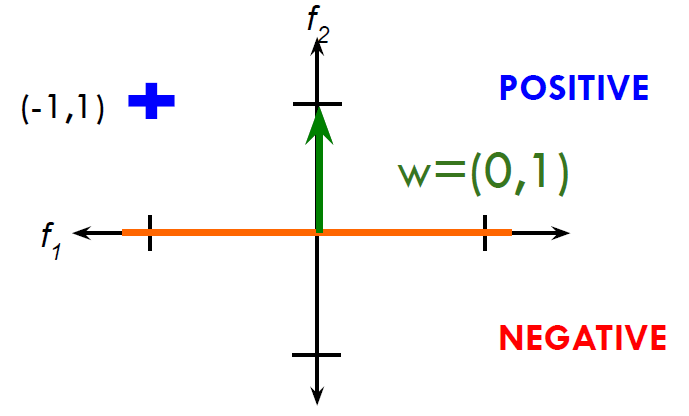
\includegraphics[width=1\linewidth]{imgs/chapter4/img3}
			\caption{Esempio: Modello aggiornato}
			\label{fig:chapter04-03}
		\end{minipage}
	\end{figure}
	
	\subsection{Perceptron}
	\`E un modello parametrico, \`e il blocco di base per la costruzioni di reti neurali.
		\subsubsection{Numero di iterazioni}
		Il numero di iterazioni del perceptron viene deciso in base alla convergenza.
		Inoltre pu\`o essere limitato in modo da ridurre l'overfitting.
		Si noti come in caso di dati non linearmente separabili la convergenza non avviene mai. 
		In caso di dati linearmente separabili abbiamo la garanzia di trovare \textbf{una} linea, non è detto che sia la migliore.
		
		\subsubsection{Ordine dei campioni}
		I campioni da considerare nel perceptron sono considerati in ordine casuale.
		In questo modo si produce un modello a low bias.
		
		\subsubsection{Linear separable sets}
		Le istanze di training sono linearmente separabili se esiste un hyperplane che separa le due classi. \ref{fig:chapter04-01}
		\begin{figure}
			\centering
			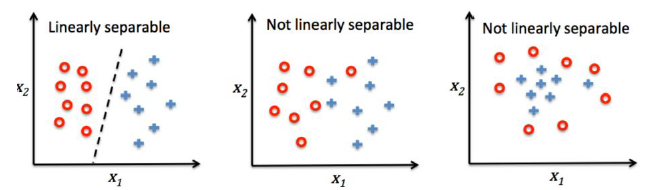
\includegraphics[width=0.6\linewidth]{imgs/chapter4/img1}
			\caption{Linear separable sets}
			\label{fig:chapter04-01}
		\end{figure}
		
		\subsubsection{Algoritmo}
		\begin{algorithm}[H]
\DontPrintSemicolon
\SetKwComment{comment}{$\%$}{}
\SetKw{Int}{int}
\SetKw{To}{to}
\SetKw{Not}{not}
\SetKwData{Item}{item}
\SetKwFunction{Min}{min}
\SetKwFunction{Perceptron}{Perceptron}

\caption{\protect\Perceptron{}}

\Repeat{Convergence}{
	\ForEach{training example ($f_1, f_2,\dots,f_n, label$)}{
		\comment{Label = $\pm 1$}
		check if it is correct based on the current label\;
		\If{\Not correct}{
			\comment{update all the weights}
			\ForEach{$w_i$}{
				$w_i\ =\ w_i\ +\ f_i\ *\ label$\;
				$b\ =\ b\ +\ label$\;
			}
		}
	}
}\comment{Or some number of iteration}



\end{algorithm}

		
		Meglio prendere esempi casuali, perch\`e l'ordine con cui prendiamo gli esempi influenza l'aggiornamento dei pesi.
		
		\subsubsection{Calcolo della predizione}
		\begin{algorithm}[H]
\DontPrintSemicolon
\SetKwComment{comment}{$\%$}{}
\SetKw{Int}{int}
\SetKw{To}{to}
\SetKw{IsNot}{is not}
\SetKw{Not}{not}
\SetKwData{Item}{item}
\SetKwFunction{Min}{min}
\SetKwFunction{Perceptron}{Perceptron}

\caption{\protect\Perceptron{}}

\Repeat{Convergence}{
	\ForEach{training example ($f_1, f_2,\dots,f_n, label$)}{
		\comment{Label = $\pm 1$}
		$prediction\ =\ b\ +\ \sum\limits_{i=1}^nw_if_i$\;
		\If{prediction \IsNot label}{
			\comment{update all the weights}
			\ForEach{$w_i$}{
				$w_i\ =\ w_i\ +\ f_i\ *\ label$\;
				$b\ =\ b\ +\ label$\;
			}
		}
	}
}\comment{Or some number of iteration}



\end{algorithm}


\section{Perceptron e reti neurali}
Si pu\`o immaginare il perceptron come un neurone artificiale o una funzione parametrizzata non lineare con un valore di attivazione soglia e un range di output ristretto.
Le reti neurali sono reti di neuroni artificiali densamente connessi in modo da simulare la rete di neuroni del cervello.

	\subsection{Funzione di attivazione}
	Una funzione di attivazione pu\`o essere una soglia dura: se la somma di tutti gli input \`e maggiore di un valore allora il perceptron manda il segnale queste permettono di imparare solo modelli lineari.
	Funzioni di attivazione pi\`u interessanti sono le sigmoidi, tangenti iperboliche, ReLU o rectified linear unit o leaky ReLU, perch\`e ci permettono di imparare modelli non lineari.
	
	\subsection{Storia del perceptron}
	Il perceptron nasce nel $1958$ da parte di Rosemblatt che lo crea con una soglia dura.
	Questo gli impedisce di imparare modelli non lineari come lo \emph{xor}.
	Viene superato nel $1986$ attraverso perceptrons multi layers e backpropagation e utilizzando una soglia meno dura.

	\chapter{Decision Trees}

\section{Struttura}
Un decision tree \`e un modello di predizione con struttura ad albero.
\`E composto da nodi terminali o foglie e nodi non terminali.
I nodi non terminali hanno da due a pi\`u figli e implementano la funzione di routing.
I nodi foglia non hanno figli e implementano la funzione di predizione.
Non ci sono cicli e tutti i nodi hanno al massimo un genitore (con esclusione del nodo radice).

\section{Funzionamento}
Un decision tree prende un input $x\in\mathcal{X}$ e lo routa attraverso i nodi fino a che raggiunge un nodo foglia dove avviene la predizione \ref{fig:chapter05-00}. 

\begin{figure}
	\centering
	\begin{minipage}{.3\textwidth}
		\centering
		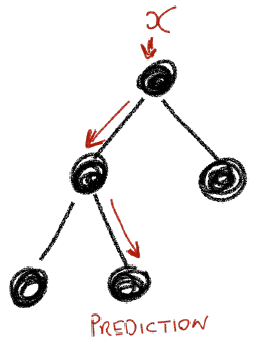
\includegraphics[width=0.7\linewidth]{imgs/chapter5/img0}
		\caption{Funzionamento}
		\label{fig:chapter05-00}
	\end{minipage}%
	\begin{minipage}{.7\textwidth}
		\centering
		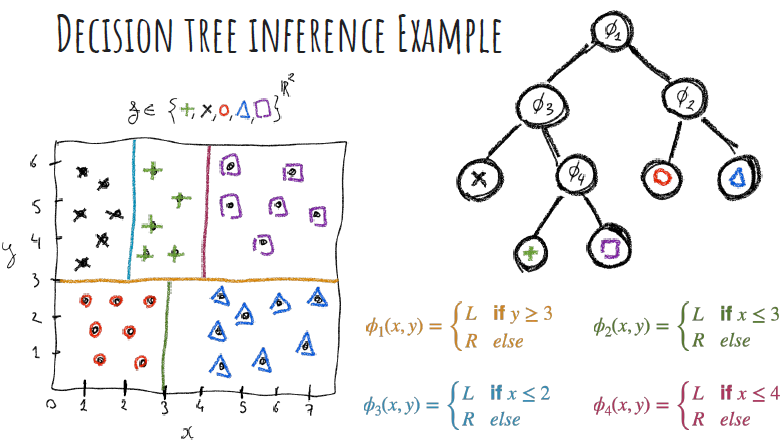
\includegraphics[width=1\linewidth]{imgs/chapter5/img1}
		\caption{Esempio inferenza DT}
		\label{fig:chapter05-01}
	\end{minipage}
\end{figure}

Ogni nodo non terminale
$$Node(\phi, t_L, t_R)$$
Contiene una funzione di routing (decisione) $\phi\in\{L, R\}^{\mathcal{X}}$, un figlio destro $t_L$ e un figlio sinistro $t_R$.
Quando $x$ raggiunge il nodo viene spostato sul figlio destro o sinistro in base al valore di $\phi(x)\in\{L,R\}$.
Ogni nodo foglia
$$Leaf(h)$$
Contiene una funzione di predizione $h\in\mathcal{F}_{task}$, tipicamente una costante. In un problema di classificazione dar\`a in ouput la classe di appartenenza. 
Quando $x$ raggiunge una foglia la previsione finale sar\`a data da: $h(x)$.

	\subsection{Inferenza}
	Sia $f_t$ la funzione che ritorna la predizione per l'input $x\in\mathcal{X}$ secondo il decision tree $t$.
	Questa viene definita ricorsivamente come:
	$$f_t(x)=\begin{cases}h(x)&\mathbf{if}\ t = Leaf(h)\\
		f_{t_{\phi(x)}}(x)&\mathbf{if}\ t = Node(\phi, t_L, t_R)
	\end{cases}$$
	I decision tree dividono lo spazio delle feature in (iper)-rettangoli (consideriamo il caso n-dimensionale), ogni regione rettangolare possiede una label \ref{fig:chapter05-01}.

\section{Decision trees learning algorithm}
Dato un training set $\mathcal{D}_n = \{z_1,\dots, z_n\}$ (dove $z_i$ \`e una coppia $(x,y)$) si deve trovare $f_{t^*}$ dove:
$$t^*\in arg\min\limits_{t\in\mathcal{T}} E(f_t;\mathcal{D}_n)$$
Dove $\mathcal{T}$ \`e l'insieme dei decision trees. 
In parole cerchiamo l'albero che minimizza l'errore.
Il problema di ottimizzazione \`e facile se non si impongono constraints(es: cercare l'albero più compatto), altrimenti potrebbe diventare \emph{NP-hard}.
Una soluzione pu\`o essere trovata utilizzando una strategia greedy.
Pertanto si assume:
$$E(f_t;\mathcal{D}) = \dfrac{1}{|\mathcal{D}|}\sum\limits_{z\in\mathcal{D}}l(f;z)$$
Il training viene svolto in modalit\`a batch.
Ora fissato un insieme di predizioni di foglie
$$\mathcal{H}_{leaf}\subset\mathcal{F}_{task}$$
E fissato un insieme di possibili funzioni di routing o split
$$\Phi\subset\{L,R\}^\mathcal{X}$$
La strategia di crescita dell'albero partiziona ricorsivamente il training set e decide se crescere foglie o nodi non terminali \ref{fig:chapter05-02}. 

\begin{figure}
	\centering
	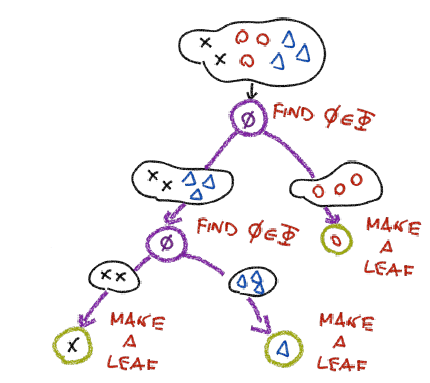
\includegraphics[width=0.4\linewidth]{imgs/chapter5/img2}
	\caption{Decision trees learning algorithm}
	\label{fig:chapter05-02}
\end{figure}


	\subsection{Crescere una foglia}
	Sia $\mathcal{D}=\{z_1, \dots, z_m\}$ il training set che raggiunge un nodo.
	Il predittore di foglia ottimale (con errore minimo) viene computato come:
	$$h^*_\mathcal{D}\in arg\min\limits_{h\in\mathcal{H}_{leaf}} E(h; \mathcal{D})$$
	Il valore di errore ottimale o misura di impurit\`a \ref{fig:chapter05-03}:
	$$I(\mathcal{D}) = E(h^*_\mathcal{D};\mathcal{D})$$
	Dove $h_\mathcal{D}$ \`e la predizione per il dataset $\mathcal{D}$.
	L'impurit\`a \`e computata nel nodo in cui arriva il sottoinsieme del dataset originale $\mathcal{D}$.
	In quel nodo si calcola il numero di errori che si farebbero classificando tutti i dati del sottoinsieme in una singola classe $c$, ripetendo il calcolo per ogni classe.
	Il numero minimo di errori che fai con una certa classe $c^*$ \`e la misura di impurit\`a del classification error.
	Se si raggiungono dei criteri si cresce una foglia $Leaf(h^*_\mathcal{D})$
	Esempi di questi criteri sono la purezza $I(\mathcal{D}) < \epsilon$, la cardinalit\`a minima $|\mathcal{D}|<k$ o un'altezza massima dell'albero.
	
	\begin{figure}
		\centering
		\begin{minipage}{.5\textwidth}
			\centering
			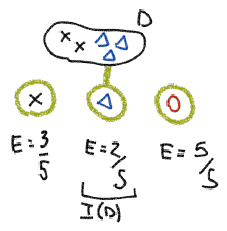
\includegraphics[width=0.6\linewidth]{imgs/chapter5/img3}
			\caption{Misura d'impurit\`a}
			\label{fig:chapter05-03}
		\end{minipage}%
		\begin{minipage}{.5\textwidth}
			\centering
			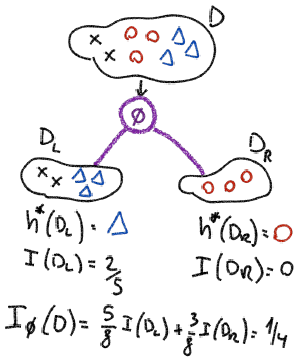
\includegraphics[width=0.6\linewidth]{imgs/chapter5/img4}
			\caption{Crescere di un nodo}
			\label{fig:chapter05-04}
		\end{minipage}
	\end{figure}
	
	\subsection{Crescere un nodo}
	Se non si raggiunge il criterio per creare una foglia si deve trovare una funzione di split ottimale:
	$$\phi^*_\mathcal{D}\in arg\min\limits_{\phi\in\Phi}I_\phi(\mathcal{D})$$
	L'impurit\`a $I_\phi(\mathcal{D})$ di una funzione di split $\phi$ dato il training set $\mathcal{D}$ viene computata nei termini di impurit\`a dei dati splittati:
	$$I_\phi(\mathcal{D})=\sum\limits_{d\in\{L,R\}}\dfrac{|\mathcal{D}^\phi_d|}{|\mathcal{D}|}I(\mathcal{D}^\phi_d)$$
	Dove
	$$\mathcal{D}^\phi_d = \{(x, y)\in\mathcal{D};\phi(x)=d\}$$
	L'impurit\`a di una funzione di split \`e il pi\`u basso errore di training che pu\`o essere ottenuto da un albero che consiste di una radice e due figlie.
	Si cresce pertanto un nodo $Node(\phi^*, t_L, t_R)$ dove $\phi^*$ \`e lo split ottimale, mentre $t_L$ e $t_R$ sono ottenuti applicando ricorsivamente l'algoritmo di learning ai training set splits \ref{fig:chapter05-04}. 
	
	\subsection{Algoritmo}
	$$Grow(\mathcal{D})=\begin{cases}Leaf(h^*_\mathcal{D}) &raggiunto\ criterio\ di\ stop\\
		Node(\phi^*_\mathcal{D}, Grow(\mathcal{D}^*_L), Grow(\mathcal{D}^*_R)) &altrimenti
	\end{cases}$$
	Dove $\mathcal{D}^*_d=\{(x, y)\in\mathcal{D};\phi^*_\mathcal{D}(x)=d\}$.
	
	\subsection{Split selection}
	Tipicamente la migliore funzione di split viene data in termini di minimizzazione dell'impurit\`a dello split, ma altre volte nella massimizzazione del guadagno di informazioni:
	$$\Delta_\phi(\mathcal{D})=I(\mathcal{D})-I_\phi(\mathcal{D})$$
	Essendo $\Delta_\phi(\mathcal{D})\ge 0$ per ogni $\phi\in\{L,R\}^{\mathcal{X}}$ e ogni training set $\mathcal{D}\subset\mathcal{X}\times\mathcal{Y}$, l'impurit\`a non aumentera mai per ogni split scelto casualmente. 
	$\Delta_\phi(\mathcal{D})$ \`e chiamato anche \emph{information gain}.
	
	\subsection{Predizione delle foglie}
	La predizione delle foglie fornisce una soluzione a un problema semplificato coinvolgendo solo dati che la raggiungono.
	Questa soluzione pu\`o essere una funzione arbitraria $h\in\mathcal{F}_{task}$, ma in pratica si restringe a un sottoinsieme di $\mathcal{H}_{leaf}$.
	Il predittore pi\`u semplice \`e una funzione che ritorna una costante (come una label).
	L'insieme di tutte le possibili funzioni costanti pu\`o essere scritto come:
	$$\mathcal{H}_{leaf} = \bigcup\limits_{y\in\mathcal{Y}}\{y\}^{\mathcal{X}}$$

\section{Misure di impurit\`a per la classificazione}
Si consideri per la classificazione:
$$\mathcal{Y} = \{c_1,\dots,c_k\}\qquad\qquad\qquad\mathcal{D}\subset\mathcal{X}\times\mathcal{Y}$$
Sia $\mathcal{D}^y = \{(x, y')\in \mathcal{D}: y = y'\}$, che denota il sottoinsieme di training samples in $\mathcal{D}$ con label $y$.
Considerando la funzione di errore:
$$E(f,\mathcal{D}) = \dfrac{1}{|\mathcal{D}|}\sum\limits_{z\in\mathcal{D}}l(f;z)$$
Se $l(f;(x,y))=1_{f(x)\neq y}$ e $\mathcal{H}_{leaf} = \bigcup\limits_{y\in\mathcal{Y}}\{y\}^\mathcal{X}$ la misura di impurit\`a \`e allora il classification error:
$$I(\mathcal{D})= 1 -\max\limits_{y\in\mathcal{Y}}\dfrac{|\mathcal{D}^y|}{|\mathcal{D}|}$$
Se invece $l(f;(x,y))=\sum\limits_{x\in\mathcal{Y}}[f_c(x)-1_{c=y}]^2$ e $\mathcal{H}_{leaf}=\bigcup\limits_{\pi\in\Delta(\mathcal{Y})}\{\pi\}^\mathcal{X}$ allora la misura di impurit\`a \`e l'impurit\`a di Gini:
$$I(\mathcal{D}) = 1-\sum\limits_{y\in\mathcal{Y}}\biggl(\dfrac{|\mathcal{D}^y|}{|\mathcal{D}|}\biggr)^2$$
Infine se $l(f;(x,y))=-\log f_y(x)$ e $\mathcal{H}_{leaf} = \bigcup\limits_{\pi\in\Delta(\mathcal{Y})}\{\pi\}^\mathcal{X}$, con una distribuzione costante di label come predizione di foglie, allora la misura di impurit\`a \`e l'entropia:
$$I(\mathcal{D})=-\sum\limits_{y\in\mathcal{Y}}\dfrac{|\mathcal{D}^y|}{|\mathcal{D}|}\log\dfrac{|\mathcal{D}^y|}{|\mathcal{D}|}$$

	\subsection{Esempio applicazione dell'algoritmo}
	\begin{multicols}{2}
		\begin{itemize}
			\item Problema di classificazione.
			\item Ottimizziamo l'errore di classificazione.
			\item Le foglie avranno una funzione di predizione che in output d\`a una costante.
			\item Le funzioni di split saranno a una dimensione.
			\item Ci fermeremo (creando una foglia) quando l'impurit\`a avr\`a raggiunto $0$.
		\end{itemize}
	\end{multicols}
	Osserviamo in figura \ref{fig:chapter05-09} come i triangoli siano i pi\`u comuni, dunque  $$I(\mathcal{D})= 1 -\max\limits_{y\in\mathcal{Y}}\dfrac{|\mathcal{D}^y|}{|\mathcal{D}|} = \frac{24}{32} > 0$$
	Poich\`e non \`e stato raggiunto il criterio per crescere una foglia, creiamo un nodo. 
	Prima per\`o dobbiamo capire qual'\`e lo split migliore \ref{fig:chapter05-10}. 
	Lo split a sinistra \`e il migliore in quanto ha l'impurit\`a pi\`u piccola. 
	Il risultato finale \`e in figura \ref{fig:chapter05-11}.
	\begin{figure}
		\centering
		\begin{minipage}{.4\textwidth}
			\centering
			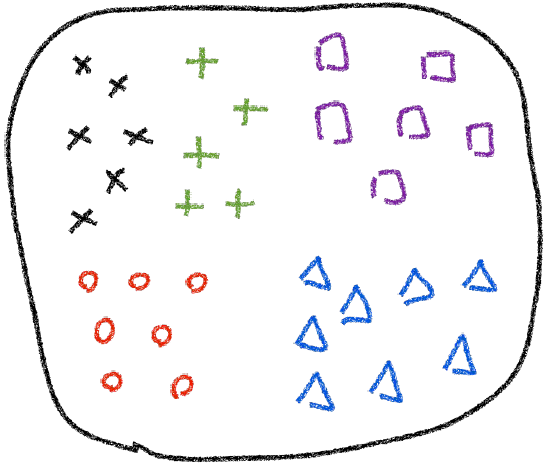
\includegraphics[width=0.8\linewidth]{imgs/chapter5/img9}
			\caption{Punto di partenza}
			\label{fig:chapter05-09}
		\end{minipage}%
		\begin{minipage}{.6\textwidth}
			\centering
			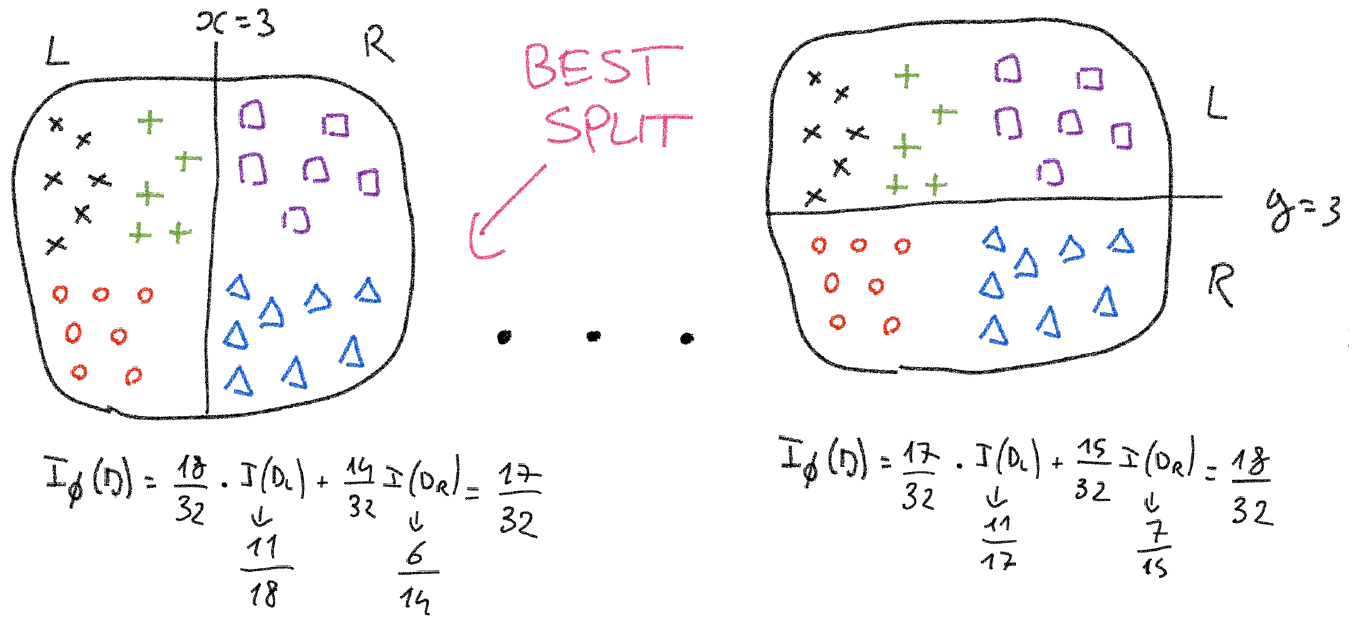
\includegraphics[width=1\linewidth]{imgs/chapter5/img10}
			\caption{Scelta dello split migliore}
			\label{fig:chapter05-10}
		\end{minipage}
	\end{figure}
	
	\begin{figure}
		\centering
		\begin{minipage}{.5\textwidth}
			\centering
			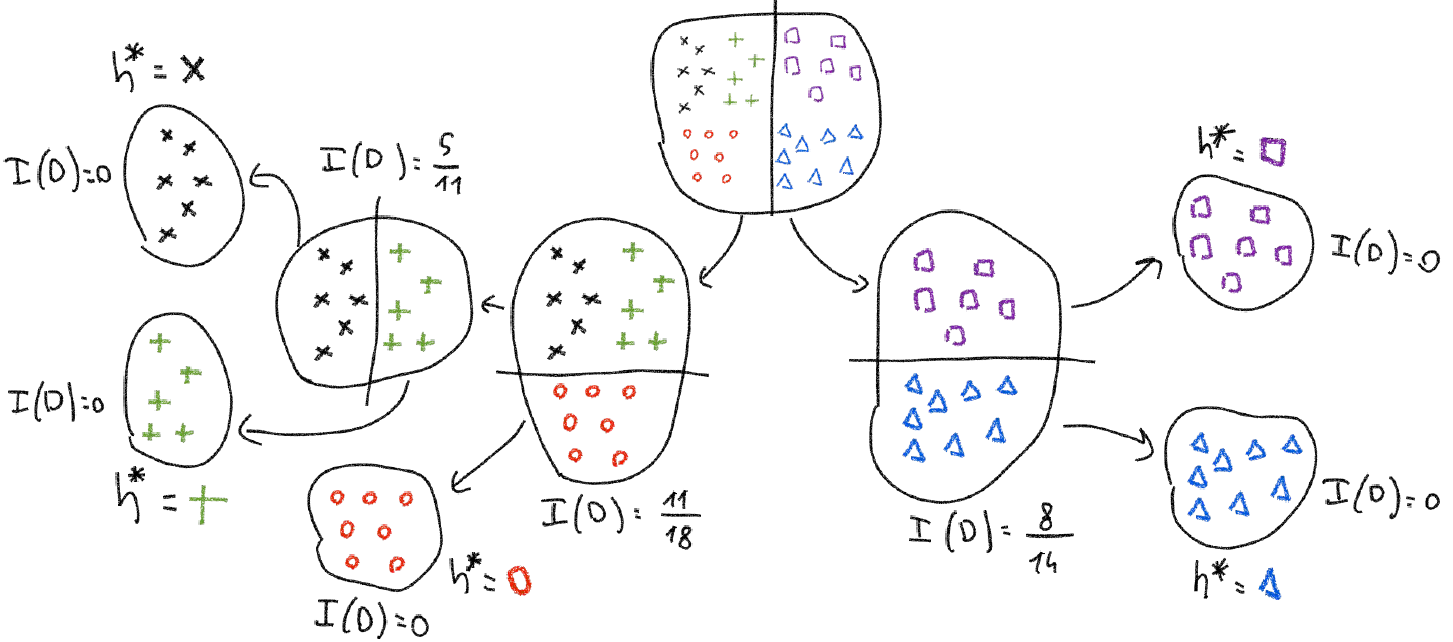
\includegraphics[width=1\linewidth]{imgs/chapter5/img11}
			\caption{Risultato finale}
			\label{fig:chapter05-11}
		\end{minipage}%
		\begin{minipage}{.5\textwidth}
			\centering
			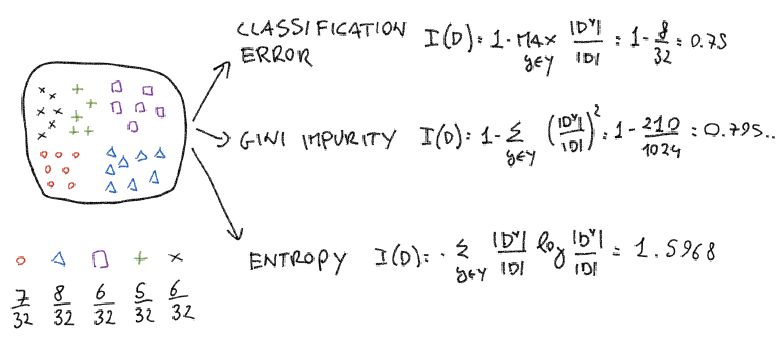
\includegraphics[width=1\linewidth]{imgs/chapter5/img5}
			\caption{Esempio misure di impurit\`a per la classificazione}
			\label{fig:chapter05-05}
		\end{minipage}
	\end{figure}

\section{Misure di impurit\`a per la regressione}
Si consideri per la regressione:
$$\mathcal{Y}\subset\mathbb{R}^d\qquad\qquad\qquad\mathcal{D}\subset\mathcal{X}\times\mathcal{Y}$$
Se $l(f;(x,y))=||f(x)-y||^2$ e $\mathcal{H}_{leaf} = \bigcup\limits_{y\in\mathcal{Y}}\{y\}^\mathcal{X}$ allora la misura di impurit\`a \`e la varianza:
$$I(\mathcal{D})=\dfrac{1}{|\mathcal{D}|}\sum\limits_{(x,y)\in\mathcal{D}}||x-\mu_\mathcal{D}||^2$$
Dove $\mu_\mathcal{D} = \frac{1}{|\mathcal{D}|}\sum\limits_{(x,y)\in\mathcal{D}}x$

\section{Data features e attributi}
Un data point $x\in\mathcal{X}$ potrebbe essere $d$ dimensionale con ogni dimensione con tipi di valori eterogenei come discreti o continui e avere un ordinamento o no, rispettivamente ordinali o nominali \ref{fig:chapter05-06}.

\begin{figure}
	\centering
	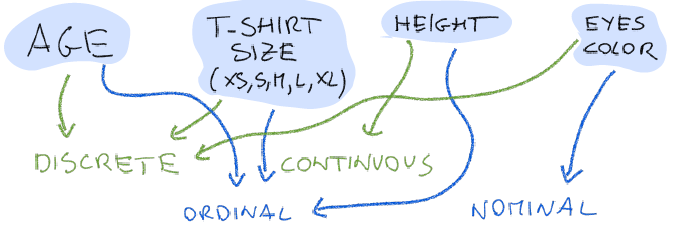
\includegraphics[width=0.6\linewidth]{imgs/chapter5/img6}
	\caption{Data features e attributi}
	\label{fig:chapter05-06}
\end{figure}

\section{Funzioni di split o routing}
Il routing o split $\phi\in\{L,R\}^{\mathcal{X}}$ determina se un data point $x\in\mathcal{X}$ deve muoversi a destra (i.e. $\phi(x)=\mathcal{R}$) o sinistra (i.e. $\phi(x)=\mathcal{L}$).
La possibile funzione di split \`e ristretta in un insieme predefinito $\Phi\subset\{L,R\}^\mathcal{X}$ in base alla natura dello spazio di features.
La funzione di split prototipica per un input $d$ dimensionale prima seleziona una dimensione e poi applica un criterio di split $1$ dimensionale.

	\subsection{Features discrete e nominali}
	Si assumano features discrete e nominali con valori in $\mathcal{K}$.
	La funzione di split pu\`o essere implementata data una partizione di $\mathcal{K}$ in $\mathcal{K}_R$ e $\mathcal{K}_L$:
	$$\phi(x) = \begin{cases}L &\mathbf{if} x\in\mathcal{K}_L\\
		R &\mathbf{if} x\in\mathcal{K}_R
	\end{cases}$$
	Trovare lo split ottimale richiede testare $2^{|\mathcal{K}|-1}-1$ bi-partizioni.
	
	\subsection{Features ordinali}
	Si assumano features ordinali con valori in $\mathcal{K}$.
	La funzione di split pu\`o essere implementata dando una soglia $r\in\mathcal{K}$:
	$$\phi(x) = \begin{cases}L &\mathbf{if} x\le r\\
		R &\mathbf{if} x>r
	\end{cases}$$
	Se $|\mathcal{K}|\le|\mathcal{D}|$ trovare lo split ottimale richiede il test di $|\mathcal{K}|-1$ soglie.
	Se $|\mathcal{K}|>|\mathcal{D}|$ si deve ordinare i valori di input in $\mathcal{D}$ dove $\mathcal{D}$ \`e il training set che raggiunge il nodo e testare $|\mathcal{D}|-1$ soglie.
	
	\subsection{Obliquo}
	A volte \`e conveniente fare split considerando pi\`u features alla volta.
	Tali funzioni lavorano con features continue e sono dette oblique in quanto generano decision boundaries obliqui.
	Se $x\in\mathbb{R}^d$ allora la funzione di split pu\`o essere implementata dato $w\in\mathbb{R}^d$ e $r\in\mathbb{R}$:
	$$\phi(x) = \begin{cases}L &\mathbf{if} w^Tx\le r\\
		R &\mathbf{altimenti}
	\end{cases}$$
	Si nota come questa funzione sia pi\`u difficile da ottimizzare.
	
	\section{Decision trees e overfitting}
	I decision trees sono modelli non parametrici con una struttura determinata dai dati.
	Per questo sono flessibili e possono facilmente fare fit sul training set, con un alto rischio di overfitting.
	Tecniche standard per migliorare la generalizzazione si applicano ai decision trees:
	\begin{multicols}{2}
		\begin{itemize}
			\item Early stopping.
			\item Regularization.
			\item Data augmentation.
			\item Complexity reduction.
			\item Ensembling.
		\end{itemize}
	\end{multicols}
	Una tecnica per ridurre la complessit\`a a posteriori \`e detta pruning.
	Se abbiamo un gran numero di attributi, possiamo trovare regolarità senza senso nei dati. 
	Oppure possiamo rimuovere anche gli attributi irrilevanti (processo manuale - non sempre possibile).

\section{Random forest}
Le random forest sono ensembles di decision trees \ref{fig:chapter05-08}.
Ogni albero \`e tipicamente trained con una versione bootstrapped del training set campionata con sostituzione.
Le funzioni di split sono ottimizzate su features campionate a caso o completamente a caso (extremely randomized trees).
Questo aiuta ad ottenere decision trees decorrelati.
La predizione finale della foresta \`e ottenuta facendo la media delle predizioni per ogni albero nell'ensemble $\mathcal{Q}=\{t_1,\dots,t_T\}$.
$$f_\mathcal{Q}(x)=\dfrac{1}{T}\sum\limits_{j=1}^Tf_t(x)$$

\begin{figure}
	\centering
	\begin{minipage}{.5\textwidth}
		\centering
		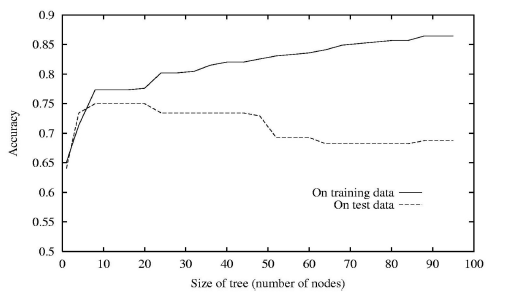
\includegraphics[width=1\linewidth]{imgs/chapter5/img7}
		\caption{Decision trees e overfitting. Aumentare il numero di nodi sui dati di training sembrava una buona idea quando non lo era sui dati di test.}
		\label{fig:chapter05-07}
	\end{minipage}%
	\begin{minipage}{.5\textwidth}
		\centering
		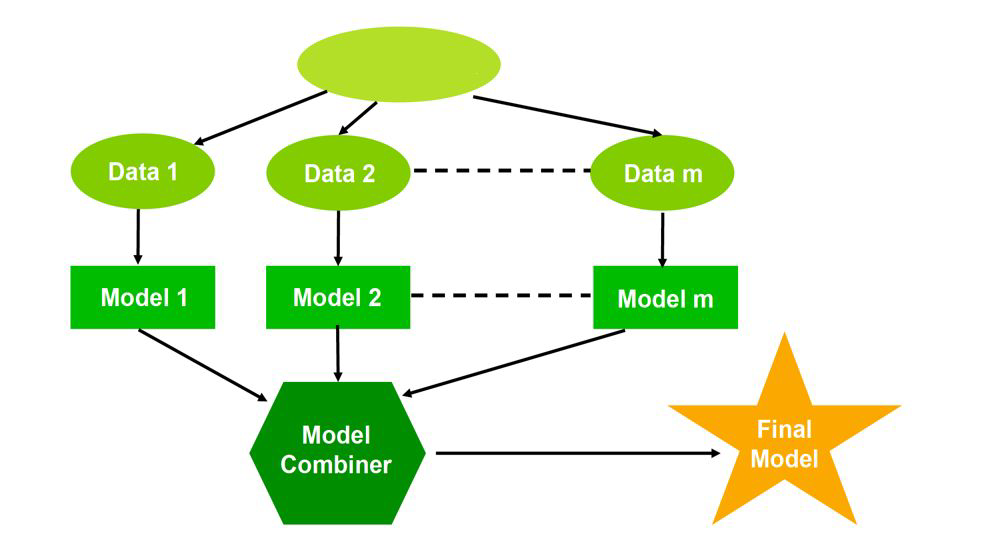
\includegraphics[width=1\linewidth]{imgs/chapter5/img8}
		\caption{Ensemble learning.}
		\label{fig:chapter05-08}
	\end{minipage}
\end{figure}

\section{Confronto con KNN}
Si nota come a differenza dei decision trees KNN non richiede nessun training, ma la classificazione \`e pi\`u veloce per i decision trees in quanto KNN per ogni esempio deve calcolare $k$ distanze.
A differenza di KNN che tratta tutte le features in maniera uguale i decision trees permettono una selezione delle features pi\`u importanti facendo scelte pesate.

	\chapter{Multi class classification}

\section{Introduzione}

	\subsection{Classificazione binaria}
	Si \`e definita la classificazione binaria come la task in cui dati:
	\begin{multicols}{2}
		\begin{itemize}
			\item Uno spazio di input $\mathcal{X}$.
			\item Una distribuzione sconosciuta $\mathcal{D}$ su $\mathcal{X}\times\{-1,+1\}$.
			\item Un training set $D$ campionato da $\mathcal{D}$
		\end{itemize}
	\end{multicols}
	Si deve computare una funzione $f$ che minimizza $\mathbb{E}_{(x,y)\sim\mathcal{D}}[f(x)\neq y]$

	\subsection{Classificazione multi classe}
	La classificazione multiclasse \`e l'estensione naturale della classificazione binaria.
	L'obiettivo \`e quello di assegnare una label discreta a degli esempi.
	La differenza \`e che ora ci sono $k>2$ classi da cui scegliere.
	Dati pertanto:
	\begin{multicols}{2}
		\begin{itemize}
			\item Uno spazio di input $\mathcal{X}$ e un numero di classi $K$.
			\item Una distribuzione sconosciuta di $\mathcal{D}$ su $\mathcal{X}\times[K]$.
			\item Un training set $D$ campionato da $\mathcal{D}$.
		\end{itemize}
	\end{multicols}
	Si deve computare una funzione $f$ che minimizza $\mathbb{E}_{(x,y)\sim\mathcal{D}}[f(x)\neq y]$.

		\subsubsection{K nearest neighbours}
		Si noti come una \emph{K-NN} per classificare un esempio $d$ trova i $k$ vicini di $d$ e sceglie la label in presenza maggiore tra i $k$ vicini pi\`u prossimi.
		Non necessita pertanto di cambi algoritmici nel caso della multi class classification.

		\subsubsection{Decision tree}
		I decision tree non richiedono cambi algoritmici per la multi class classification.

	\subsection{Approccio black box alla multi class classification}
	Dato un classificatore binario questo si pu\`o usare per risolvere il problema della multiclass classification.
	Si noti come un perceptron oltre al risultato pu\`o anche dare un punteggio di confidenza.
	Inoltre siccome una linea non \`e sufficiente per dividere le classi se ne possono usare diverse.

\section{One versus all \emph{OVA}}
Nell'approccio \emph{OVA} nel training si definisce per ogni label $L$ un problema binario in cui:
\begin{multicols}{2}
	\begin{itemize}
		\item Tutti gli esempi con la label $L$ sono positivi.
		\item Tutti gli altri esempi sono negativi.
	\end{itemize}
\end{multicols}
In pratica si imparano $L$ diversi modelli di classificazione.
Si ricordi come il classificatore divide il piano in due semipiani.

	\subsection{Ambiguit\`a}
	In questo caso si formano pertanto delle zone in cui si creano delle ambiguit\`a.
	Se il classificatore non fornisce confidence e c'\`e ambiguit\`a si sceglie una delle label in conflitto.
	Nella maggior parte dei casi i classificatori forniscono confidence, allora in questo caso si:
	\begin{multicols}{2}
		\begin{itemize}
			\item Si sceglie il positivo con confidence maggiore.
			\item Se nessuno \`e positivo si sceglie il negativo con confidence minore.
		\end{itemize}
	\end{multicols}
	La confidence nel perceptron si calcola come distanza dall'iperpiano stabilito dalla prediction.

	\subsection{Algoritmi}
	
\begin{algorithm}
\DontPrintSemicolon
\SetKwComment{comment}{$\%$}{}
\SetKw{Int}{int}
\SetKw{To}{to}
\SetKw{IsNot}{is not}
\SetKw{Not}{not}
\SetKw{Return}{Return}
\SetKwData{Item}{item}
\SetKwFunction{BinaryTrain}{BinaryTrain}
\SetKwFunction{Ova}{OneVersusAllTrain}

\caption{\protect\Ova{$D^{multiclass}$, \protect\BinaryTrain{}}}

\For{$i\ =\ 1$ \To $K$}{
	$D^{bin}$ = relabel $D^{multiclass}$ in modo che $i$ \`e positivo e $\neq i$ \`e negativo\;
	$f_i$ = \BinaryTrain{$D^{bin}$}\;
}
\Return $f_1,\dots, f_K$

\end{algorithm}

	\begin{algorithm}[H]
\DontPrintSemicolon
\SetKwComment{comment}{$\%$}{}
\SetKw{Int}{int}
\SetKw{To}{to}
\SetKw{IsNot}{is not}
\SetKw{Not}{not}
\SetKw{Return}{Return}
\SetKwData{Item}{item}
\SetKwFunction{BinaryTrain}{BinaryTrain}
\SetKwFunction{Ova}{OneVersusAllTest}
\SetKwFunction{Max}{max}

\caption{\protect\Ova{$f_1,\dots,f_K$, $\hat{x}$}}

score = $\langle 0,\dots, 0\rangle$		\comment{Inizializza $K$ score a $0$}

\For{$i\ =\ 1$ \To $K$}{
	y = $f_i(\hat{x})$\;
	$score_i\ =\ score_i + y$\;
}
\Return \Max{score}\;

\end{algorithm}


\section{All versus all \emph{AVA}}
Un approccio alternativo consiste nel gestire il problema della classificazione multi classe decomponendolo in problemi di classificazione binaria.
Questo approccio viene detto anche all pairs.
Si classificano $\frac{K(K-1)}{2}$ classificatori in modo che
$$F_{ij}, 1\le i< j \le K$$
Sia il classificatore che discrimina la classe $i$ contro la classe $j$.
Questo classificatore riceve tutti gli esempi della classe $i$ come positivi e tutti gli esempi della classe $j$ come negativi.
Quando arriva un punto di test si valuta su tutti i classificatori $F_{ij}$.
Ogni volta che $F_{ij}$ predice positivo la classe $i$ prende un voto, altrimenti lo prende $j$.
Dopo aver eseguito tutti i $\frac{K(K-1)}{2}$ classificatori la classe con pi\`u voti decide la label.

	\subsection{\emph{AVA} training}
	Per ogni coppia di label si addestra un classificatore che le distingue:
	\begin{algorithm}[H]
\DontPrintSemicolon
\SetKwComment{comment}{$\%$}{}
\SetKw{Int}{int}
\SetKw{To}{to}
\SetKw{IsNot}{is not}
\SetKw{Not}{not}
\SetKw{Return}{Return}
\SetKwData{Item}{item}
\SetKwFunction{BinaryTrain}{BinaryTrain}
\SetKwFunction{Ava}{AllVersusAllTrain}
\SetKwFunction{Max}{max}

\caption{\protect\Ava{}}
\For{i = 1 \To number of labels}{
	\For{j = i + 1 \To number of labels}{
		train a classifier $F_{ij}$ to distinguish between $label_j$ and $label_i$\;
		create a dataset with all examples with $label_j$ labeled positive and with $label_i$ negative\;
		Train classifier $F_{ij}$ su questo sottoinsieme di dati\;
	}
}
\end{algorithm}


	\subsection{\emph{AVA} classification}
	Per classificare un esempio $x$ lo si classifica per ogni classificatore $F_{ij}$.
	Per scegliere la classe finale si pu\`o:
	\begin{multicols}{2}
		\begin{itemize}
			\item Considerare la maggioranza.
			\item Considerare un voto pesato basato sulla confidence:
				\begin{itemize}
					\item $y = F_{ij}(x)$.
					\item $score_j +=y$.
					\item $score_i -=y$.
				\end{itemize}
				Lo score viene cambiato in quanto se $y$ \`e positivo il classificatore lo pensa di tipo $j$, se negativo lo pensa di tipo $i$ e pertanto lo score viene aggiornato di conseguenza.
		\end{itemize}
	\end{multicols}

	\subsection{Algoritmi}
	\begin{algorithm}
\DontPrintSemicolon
\SetKwComment{comment}{$\%$}{}
\SetKw{Int}{int}
\SetKw{To}{to}
\SetKw{IsNot}{is not}
\SetKw{Not}{not}
\SetKw{Return}{Return}
\SetKwData{Item}{item}
\SetKwFunction{BinaryTrain}{BinaryTrain}
\SetKwFunction{Ava}{AneVersusAllTrain}

\caption{\protect\Ava{$D^{multiclass}$, \protect\BinaryTrain{}}}
$f_{ij}\ =\ \emptyset,\ \forall 1\le i < j \le K$\;
\For{$i\ =\ 1$ \To $K\ -\ 1$}{
	$D^{pos}\ =\ $ all $x\in D^{multiclass}$ labeled $i$\;
	\For{$j\ =\ j\ +\ 1$ \To $K$}{
		$D^{neg}\ =$ all $x\in D^{multiclass}$ labeled $j$\;
		$D^{bin}\ =\ \{(x, +1):x\in D^{pos}\}\cup\{(x,-1):x\in D^{neg}\}$\;
		$f_{ij}$ = \BinaryTrain{$D^{bin}$}\;
	}
}

\Return all $f_{ij}$

\end{algorithm}

	\begin{algorithm}[H]
\DontPrintSemicolon
\SetKwComment{comment}{$\%$}{}
\SetKw{Int}{int}
\SetKw{To}{to}
\SetKw{IsNot}{is not}
\SetKw{Not}{not}
\SetKw{Return}{Return}
\SetKwData{Item}{item}
\SetKwFunction{BinaryTrain}{BinaryTrain}
\SetKwFunction{Ava}{AllVersusAllTest}
\SetKwFunction{Max}{max}

\caption{\protect\Ava{all $f_{ij}$, $\hat{x}$}}

score = $\langle 0,\dots, 0\rangle$		\comment{Inizializza $K$ score a $0$}

\For{$i\ =\ 1$ \To $K\ -\ 1$}{
	\For{$j\ =\ i\ +\ 1$ \To $K$}{
		y = $f_{ij}(\hat{x})$\;
		$score_i\ =\ score_i + y$\;
		$score_j\ =\ score_j - y$\;
	}
}
\Return \Max{score}\;

\end{algorithm}


\section{Confronto tra \emph{OVA} e \emph{AVA}}

	\subsection{Tempo di training}
	\emph{AVA} impara pi\`u classificatore ma il training set \`e omlto pi\`u piccolo pertanto tende ad essere pi\`u veloce se le label sono equamente bilanciate.

	\subsection{Tempo di test}
	Avendo \emph{AVA} pi\`u classificatori \`e tipicamente pi\`u lenta.

	\subsection{Errori}
	\emph{AVA} fa training con data sets pi\`u bilanciata, ma avendo pi\`u classificatori i test tendono ad avere pi\`u possiblit\`a di errori.

\section{Riassunto}
Se vengono usati classificatori binari viene tipicamente utilizzata  \emph{OVA}, altrimenti si usa un classificatore che permette label multiple come \emph{DT} o \emph{K-NN}, nonostante altri metodi pi\`u sofisticati siano meglio.

\section{Multiclass evaluation}

	\subsection{Microaveraging}
	Nel microaveraging si fa la media sugli esempi.

	\subsection{Macroaveraging}
	Nel macroaveraging si calcola lo score di valutazione o accuratezza per ogni label e poi si fa la media tra le label.
	Questo in quanto d\`a pi\`u enfasi a label pi\`u rare e permette un'altra dimensione di analisi.

	\subsection{Confusion matrix}
	La confusion matrix \`e una matrice in cui $(i, j)$ rappresenta il numero di esempi con label $i$ predetti avere label $j$.
	Viene spesso espressa come percentuale.

	\chapter{Ranking}

\section{Classificazione multiclasse e multilabel}
Nella classificazione multi classe ogni esempio ha esattamente una label che sono pertanto mutualmente esclusive.
Nella classificazione multi label ogni esempio ha zero o pi\`u labels, dette anche annotazioni.
Per svolgere una classficazione multi label basterebbe fare training su un modello per ogni label e applicarli a ogni nuovo esempio, ma ci sono altri metodi pi\`u sofisticati ed efficaci come il joint learning.

\section{Problema del ranking}
I dati di training sono divisi in $K$ categoria ognuna delle quali corrispondente a un ranking.
Si deve insegnare a un modello che quando riceve un insieme di esempi li fitti nel ranking corretto o ritorni un ordinamento per questo nuovo esempio.

	\subsection{Preference function}
	La preference function o binary classifier \`e un'implementazione di ranking.
	Data una query $q$ e due campioni $x_i$ e $x_j$ il classificatore predice se $x_i$ deve essere preferito a $x_j$ rispetto alla query $q$.
	Il classificatore prende pertanto due campioni e d\`a in output $1$ se il primo \`e pi\`u alto o $-1$ se \`e pi\`u basso.
	In questo modo si ottiene una funzione di ordinamento atomica che si pu\`o estendere a diversi esempi.

		\subsubsection{Perceptron}
		Per implementare questo algoritmo si pu\`o utilizzare il perceptron creando il vettore delle feature combinate dei due esempi:
		$$f'_i = a_i -b_i$$
		$$f'_i = \begin{cases}1\ if\ a_i > b_i\\0\ altrimenti\end{cases}$$
		Questa funzione viene sviluppata in maniera dipendente dall'applicazione.
		Un modo per computare il ranking numerico per i campioni pu\`o essere risolto utilizzando la preference function sommando i valori di ritorno di ogni classificatore e ottenendo uno score per ognuno di essi.

\section{Utilizzo del ranking e della preference function}
Con gli algoritmi visti precedentemente si potrebbe pesare il ranking di un esempio utilizzando la distanza dagli altri.
Si possono usare diversi metodi di distanza dati che sono consistenti.
La distanza a tempo di testing \`e calcolata come la confidenza della predizione del perceptron e d\`a un ordinamento degli esempi.
In questo modo si ottiene una forma di ranking pi\`u precisa rispetto a quella vista prima.
Per un algoritmo di ranking sofisticato si devono incorporare queste osservazioni a tempo di training: se un problema ritorna un'alta differenza in preferenza tra due esempi dovrebbe avere un peso pi\`u alto.

\section{Naive Ranking}

	\subsection{Training}
	\begin{algorithm}[H]
\DontPrintSemicolon
\SetKwComment{comment}{$\%$}{}
\SetKw{Int}{int}
\SetKw{To}{to}
\SetKw{IsNot}{is not}
\SetKw{Is}{is}
\SetKw{Not}{not}
\SetKw{Return}{return}
\SetKw{And}{and}
\SetKw{Require}{return}
\SetKwData{Item}{item}
\SetKwFunction{Min}{min}
\SetKwFunction{BinaryTrain}{BinaryTrain}
\SetKwFunction{NRT}{NaiveRankTrain}

\caption{\protect\NRT{RankingData, \protect\BinaryTrain}}
$D = []$\;
\For{$n = 1$ \To $N$}{
	\For{all $i,j = 1$ to $M$ \And $i\neq j$}{
		\If{$i$ \Is prefered to $j$ on query $n$}{
			$D = D\oplus (x_{nij},-1)$
		}
	}
}
\Return \BinaryTrain{D}
\end{algorithm}


	\subsection{Testing}
	\begin{algorithm}[H]
\DontPrintSemicolon
\SetKwComment{comment}{$\%$}{}
\SetKw{Int}{int}
\SetKw{To}{to}
\SetKw{IsNot}{is not}
\SetKw{Is}{is}
\SetKw{Not}{not}
\SetKw{Return}{return}
\SetKw{And}{and}
\SetKw{Require}{return}
\SetKwData{Item}{item}
\SetKwFunction{Min}{min}
\SetKwFunction{BinaryTrain}{BinaryTrain}
\SetKwFunction{NRT}{NaiveRankTest}
\SetKwFunction{Argsort}{ArgSort}

\caption{\protect\NRT{$f$, $\hat{x}$}}
$score = \langle 0,\dots, 0\rangle$\;
\For{all $i,j = 1$ \To $M$ \And $i\neq j$}{
	$y = f(\hat{x}_{ij})$\;
	$score_i = score_i + y$\;
	$score_j = score_j - y$\;
}
\Return \Argsort{score}
\end{algorithm}


\section{Bipartite ranking}
Gli algoritmi di ranking bipartito risalgono problemi in cui si tenta di predire una risposta binaria.
L'obiettivo \`e di assicurare che tutti gli esempi rilevanti si trovano prima di quelli irrilevanti.
Non si trova un ordinamento tra esempi rilevanti.


\section{Ordinamento e $\mathbf{\omega}$-ranking}
Nonostante la veloce soluzione dell'ordinamento contro la funzione di preference si pu\`o utilizzarla come funzione di sorting.
Si definisce un ranking come una funzione $\sigma$ che mappa gli oggetti alla posizione nella lista di ranking desiderata $(1,\dots,M)$.
Se $\sigma_u < \sigma_v$ allora $u$ \`e preferito a $v$.
Dati i dati con ranking osservati $\sigma$ l'obiettivo \`e di imparare a predire i ranking per nuovi oggetti $\sigma^*$.
Si definisce $\sum_M$ l'insieme di tutti gli ordinamenti di ranking in $M$.
Si vuole modellare il fatto che uno sbaglio su alcune coppie \`e peggiore rispetto ad altre, pertanto si implementa una nuova funzione di errore per questo scopo.
Si definisce una funzione di costo $\omega$ dove $\omega(i,j)$ \`e il costo di mettere qualcosa nella posizione $j$ quando dovrebbe essere in $i$.
Tale funzione deve essere:
\begin{multicols}{2}
	\begin{itemize}
		\item Simmetrica: $w(i,j) = w(j,i)$.
		\item Monotona: $i<j<l\lor i>j>k \Rightarrow \omega(i,j) \le \omega(i,k)$.
		\item Soddisfi la disuguaglianza triangolare: $\omega(i,j)+\omega(j,k) \le \omega(i,k)$.
	\end{itemize}
\end{multicols}
Un esempio potrebbe essere:
$$\omega(i,j) = \begin{cases}1\ if\{i,j\} \le K \land i\neq j\\ 0\ altrimenti\end{cases}$$
Questa viene detta task di $\omega$ ranking.
Dati:
\begin{multicols}{2}
	\begin{itemize}
		\item Uno spazio di input $\mathcal{X}$.
		\item Una distribuzione sconosciuta $\mathcal{D}$ su $\mathcal{X}\times\sum_M$.
		\item Un training set $D$ campionato da $\mathcal{D}$.
	\end{itemize}
\end{multicols}
Si deve computare una funzione $f:\mathcal{X}\rightarrow\sum_M$ che minimizzi:
$$\mathbb{E}_{(\mathcal{X},\sigma)\sim\mathcal{D}}\biggl[\sum\limits_{u\neq v}[\sigma_u < \sigma_v][\hat{\sigma}_v < \hat{\sigma}_u]\omega(\sigma_u,\sigma_v)\biggr]$$
Dove $\hat{\sigma} = f(x)$.

	\subsection{Testing}
	A tempo di testing invece di predirre score e poi ordinare la lista come negli algoritmi prima si utilizza un algoritmo di ordinamento utilizzando la funzione imparata come funzione di ordinamento.
	In pratica ad ogni passo si sceglie un pivot $p$ e ogni oggetto $u$ viene confrontato con $p$ utilizzando la funzione imparata e ordinato a destra o a sinistra.
	La differenza \`e che qua la funzione di comparazione \`e probabilistica.

	\subsection{Implementazione}

		\subsubsection{Algoritmo di train}
		
\begin{algorithm}[H]
\DontPrintSemicolon
\SetKwComment{comment}{$\%$}{}
\SetKw{Int}{int}
\SetKw{To}{to}
\SetKw{IsNot}{is not}
\SetKw{Is}{is}
\SetKw{Not}{not}
\SetKw{Return}{return}
\SetKw{And}{and}
\SetKw{Require}{return}
\SetKwData{Item}{item}
\SetKwFunction{Min}{min}
\SetKwFunction{BinaryTrain}{BinaryTrain}
\SetKwFunction{NRT}{OmegaRankTest}
\SetKwFunction{Argsort}{ArgSort}
\SetKwFunction{Sign}{Sign}

\caption{\protect\NRT{$D^{rank}$, $\omega$, \protect\BinaryTrain}}
$D^{bin} = []$
\For{all $(x,\sigma)\in D^{rank}$}{
	\For{all $u\neq v$}{
		$y =$ \Sign{$\sigma^v$, $\sigma_u$}\;
		$w = w(\sigma_u, \sigma_v)$\;
		$D^{bin} = D^{bin}\oplus(y, w, x_{uv})$\;
	}
}
\Return \BinaryTrain{$D^{bin}$}
\end{algorithm}


		\subsubsection{Algoritmo di test}
		\begin{algorithm}[H]
\DontPrintSemicolon
\SetKwComment{comment}{$\%$}{}
\SetKw{Int}{int}
\SetKw{To}{to}
\SetKw{IsNot}{is not}
\SetKw{Is}{is}
\SetKw{Not}{not}
\SetKw{Return}{return}
\SetKw{And}{and}
\SetKw{Or}{or}
\SetKw{Require}{return}
\SetKwData{Item}{item}
\SetKwFunction{Min}{min}
\SetKwFunction{BinaryTrain}{BinaryTrain}
\SetKwFunction{NRT}{OmegaRankTest}
\SetKwFunction{Argsort}{ArgSort}

\caption{\protect\NRT{$f$, $\hat{x}$, obj}}
\If{obj contains $0$ \Or $1$ elements}{
	\Return obj
}
\Else{
	$p = $randomply chosen object in obj\;
	$left = []$\;
	$right = []$\;
	\For{all $u\in obj\backslash\{p\}$}{
		$\hat{y} = f(x_{up})$\;
		\If{uniform random variable $< \hat{y}$}{
			$left = left\oplus u$\;
		}
		\Else{
			$right = right\oplus u$\;
		}
	}
	$left = $\NRT{$f$, $\hat{x}$, $left$}\;
	$right = $\NRT{$f$, $\hat{x}$, $right$}\;
	\Return $left\oplus\langle p \rangle\oplus right$\;
}


\end{algorithm}


	\chapter{Gradient descent}

\section{Model based machine learning}
Nel model based machine learning si sceglie un modello definito da un insieme di parametri.
In particolare si nota come:
\begin{multicols}{2}
	\begin{itemize}
		\item Per i decision trees i parametri sono la struttura dell'albero, quali features ogni nodo divide e le predizioni delle foglie.
		\item Per il perceptron i parametri sono i pesi e il valore di $b$.
	\end{itemize}
\end{multicols}
Dopo aver scelto il modello si deve scegliere un criterio da ottimizzare o la funzione obiettivo come per esempio il training error.
Infine si sviluppa un algoritmo di learning che deve cercare di minimizzare il criterio, spesso in maniera euristica.

	\subsection{Modelli lineari}
	Nei modelli lineari il modello \`e:
	$$0=b+\sum\limits_{j=1}^mw_jf_j$$
	Si deve scegliere il criterio da ottimizzare.

		\subsubsection{Notazioni}

			\paragraph{Funzione indicatrice}
			Una funzione indicatrice trasforma valori di \emph{Vero} e \emph{Falso} in numeri e li conteggia.
			$$1[x]=\begin{cases}1&\mathbf{if}\ x = True\\
										  	0&\textbf{if}\ x = False
				 	\end{cases}$$

			\paragraph{Dot-product}
			Utilizzando una notazione vettoriale si rappresenta un esempio $f_1,\dots,f_m$ come un vettore singolo $\overrightarrow{x}$ in cui $j$ indicizza la feature e $i$ indicizza un dataset di esempi.
			Si possono rappresentare anche i pesi $w_1,\dots,w_m$ come un vettore $\overrightarrow{w}$.
			Il dot-product tra due vettori $a$ e $b$ viene definito come:
			$$a\cdot b = \sum\limits_{j=1}^ma_jb_j$$

		\subsubsection{Funzione obiettivo}
		Il criterio da ottimizzare o funzione obiettivo pu\`o essere:
		$$\sum\limits_{i=1}^n1[y_i(w\cdot x_i+b)\le 0]$$
		Si devono pertanto trovare $w$ e $b$ tali che minimizzano questa funzione, ovvero:
		$$argmin_{w,b}\sum\limits_{i=1}^n1[y_i(w\cdot x_i+b)\le 0]$$

\section{Loss functions}

	\subsection{Loss $0/1$}
	Una funzione di loss $0/1$ \`e una funzione nella forma:
	$$\sum\limits_{i=1}^n1[(y_i*w\cdot x_i+b)\le 0]$$
	Dove tra le quadre si trova se la predizione e la label sono d'accordo, con vero se non lo fanno e tra le tonde la distanza dall'iperpiano, di cui il segno \`e la predizione.
	Questa funzione ritorna il numero di sbagli.

		\subsubsection{Minimizzare la loss $0/1$}
		Per minimizzare una funzione $0/1$ si deve, ogni volta cambiare un valore di $w$ in modo che l'esempio \`e corretto o scorretto la perdita aumenta o diminuisce.
		Si nota come a ogni feature aggiunta si aggiunge una nuova dimensione allo spazio.
		Il minimo si trova trovando $w$ e $b$ che minimizzano la perdita.
		Questo \`e un problema \emph{NP-hard}.
		Sue difficolt\`a comprendono il fatto che piccoli cambi in ogni $w$ possono portare a grandi cambi nella perdita in quanto il cambio non \`e continuo.
		Ci possono essere molti minimi locali.
		Ad ogni punto non si hanno informazioni che direzionano verso il minimo.
		Pertanto si nota come una loss function ideale sia continua e differenziabile in modo da avere un'indicazione verso la direzione di minimizzazione e un unico minimo.

			\paragraph{Loss function ideale}
			Una loss function ideale dovrebbe essere:
			\begin{itemize}
				\item Continua in modo da ottenere informazioni riguardo la direzione della minimizzazione.
				\item Avere un solo minimo.
				\item Misurare la distanza tra la predizione reale e quella predetta.
			\end{itemize}

	\subsection{Funzioni convesse}
	In una funzione convessa il segmento tra qualsiasi due punti della funzione si trova al di sopra della funzione.

	\subsection{Surrogate loss function}
	Per molte applicazioni si vuole minimizzare la loss $0/1$.
	Una surrogate loss function \`e una loss function che fornisce un limite superiore alla loss function attuale.
	Si vuole identificare un surrogato convesso della loss function in modo da facilitarne la minimizzazione.
	Chiave a una loss function \`e come verifica la differenza tra la label $y$ effettiva e la predizione $y'$.

		\subsubsection{Alcune surrogate loss function}
		\begin{multicols}{2}
			\begin{itemize}
				\item \emph{$01$ loss}: $l(y, y')=1[yy'\le 0]$.
				\item \emph{Hinge} $l(y,y')=\max(0,1-yy')$.
				\item Exponential: $l(y,y')=\exp(-yy')$
				\item \emph{Squared loss}: $l(y,y')=(y-y')^2$.
			\end{itemize}
		\end{multicols}

\section{Gradient descent}
Il gradient descent \`e un modo per trovare il minimo di una funzione: le derivate parziali danno un slope o direzione dove muoversi in tale dimensione.
Questo approccio consiste di scegliere un punto di partenza e a ripetizione di: scegliere una dimensione e muoversi di una piccola quantit\`a verso il minimo utilizzando la derivata.
Pertanto si:
\begin{itemize}
	\item Sceglie un punto di inizio $w$.
	\item Sceglie una dimensione.
	\item si muove di una piccola quantit\`a verso la diminuzione della loss utilizzando la derivata.
\end{itemize}
Questo ciclo si ripete fino a che la loss non diminuisce in nessuna dimensione.

	\subsection{Spostamento in direzione della minimizzazione dell'errore}
	Il movimento in direzione della minimizzazione dell'errore \`e pertanto:
	$$w_j = w_j - \eta \dfrac{d}{dw_i}loss(w)$$
	Dove $\eta$ \`e il learning rate.

		\subsubsection{Calcolo dello spostamento per la loss function esponenziale}
		Si deve pertanto calcolare:
		\begin{align*}
			\dfrac{d}{dw_j}loss &=\dfrac{d}{dw_j}\sum\limits_{i=1}^n\exp(-y_i(w\cdot x_i + b))=\\
												 &=\sum\limits_{i=1}^n\dfrac{d}{dw_j}[-y_i(w\cdot x_i+b)]\exp(-y_i(w\cdot x_i+b))\\
		\end{align*}
		Si consideri pertanto ora:
		\begin{align*}
			\dfrac{d}{dw_j}[-y_i(w\cdot x_i + b)]&=-\dfrac{d}{dw_j}[-y_i(w\cdot x_i + b)]=\\
																		&=-\dfrac{d}{dw_j}y_i(w_1x_{i1}+\cdots+w_mx_{im}+b)=\\
																		&=-y_ix_{ji}
		\end{align*}
		Si nota pertanto come:
		$$\dfrac{d}{dw_j}loss=\sum\limits_{i=1}^n-y_ix_{ij}\exp(-y_i(w\cdot x_i+b))$$
		Si aggiorna pertanto $w_j$:
		$$w_j=w_j-\eta\sum\limits_{i=1}^n-y_ix_{ij}\exp(-y_i(w\cdot x_i+b))$$
		Questo viene fatto per ogni esempio $x_i$.

	\subsection{Learning algorithm del perceptron}
	Si nota pertanto come considerando il perceptron nell'ambito del gradient descent si aggiorna sempre il vettore dei pesi.\\
	\begin{algorithm}[H]
\DontPrintSemicolon
\SetKwComment{comment}{$\%$}{}
\SetKw{Int}{int}
\SetKw{To}{to}
\SetKw{IsNot}{is not}
\SetKw{Not}{not}
\SetKwData{Item}{item}
\SetKwFunction{Min}{min}
\SetKwFunction{Perceptron}{Perceptron}

\caption{\protect\Perceptron{}}

\Repeat{Convergence}{
	\ForEach{training example ($f_1, f_2,\dots,f_n, label$)}{
		\comment{Label = $\pm 1$}
		$prediction\ =\ b\ +\ \sum\limits_{i=1}^nw_if_i$\;
			\ForEach{$w_i$}{
				$w_j = w_j + \eta y_ix_{ij}\exp(-y_i(w\cdot x_i + b))$
				$b\ =\ b\ +\ label$\;
			}
		}
	}



\end{algorithm}

	Si noti come in questo caso $\eta$ rappresenta il learning rate, $y_i$ la label e $(w\cdot x_i + b))$ la predizione.
	Questi generano una costante $c$

	\subsection{Costante $\mathbf{c}$}
	Nella costante $c$ se label e predizione hanno lo stesso segno quando gli elementi predetti aumentano gli aggiornamenti diventano minori.
	Se invece sono diversi pi\`u diversi lo sono, maggiore l'aggiornamento.

	\subsection{Gradiente}
	Il gradiente \`e il vettore delle derivate parziali rispetto a tutte le coordinate dei pesi:
	$$\nabla L = \biggl[\dfrac{\partial L}{\partial w_1}\cdots\dfrac{\partial L}{\partial w_N}\biggr]$$
	Ogni derivata parziale misura quanto veloce la perdita cambia in una direzione.
	Quando il gradiente \`e zero la perdita non sta cambiando in nessuna direzione.\\
	
\begin{algorithm}
\DontPrintSemicolon
\SetKwComment{comment}{$\%$}{}
\SetKw{Int}{int}
\SetKw{To}{to}
\SetKw{IsNot}{is not}
\SetKw{Not}{not}
\SetKw{Return}{return}
\SetKwData{Item}{item}
\SetKwFunction{Min}{min}
\SetKwFunction{GradientDescent}i{GradientDescent}

\caption{\protect\GradientDescent{$\mathcal{F}$, $K$, $\eta_1$, $\dots$}}
	$z^{(0)}\ \rightarrow <0,0,\dots,0$\comment{Inizializza la variabile da ottimizzare}
	\For{$k = 1$ \To $K$}{
		$g^{(k)}\ \rightarrow\ \nabla_z\mathcal{F}|_{z^{(k-1)}}$\comment{Computa il gradiente nella posizione corrente}
		$z^{(k)} \rightarrow z^{(k-1)} - \eta^{(k)}g^{(k)}$\comment{scendi il gradiente}
	}
	\Return $z^{(k)}$\end{algorithm}

	Nei problemi in cui il problema di ottimizzazione \`e non convesso si trovano dei minimi locali, questi non permettono all'algoritmo di proseguire in quanto non distingue tra minimi locali e minimi globali.
	Un altro punto \`e un punto a sella, in cui certe direzioni curvano verso l'alto e altre verso il basso.
	In tali punti il gradiente \`e $0$ e l'algoritmo si blocca.
	Un modo per uscire da un punto \`a sella \`e spostarsi a lato un po' in modo da uscirne.
	Si nota come i punti a sella sono molti comuni in alte dimensioni.
	Il learning rate \`e molto importante in quanto permette di decidere la distanza coperta da uno spostamento determinando velocit\`a di avvicinamento al minimo e precisione dell'algoritmo.

	\chapter{Regularization}

\section{Introduzione}
Si noti come con il gradient descent si calcola il valore minimo della loss function sul training set.
Ci si deve pertanto preoccupare del overfitting.
Il minimo $w$ e $b$ sul training set infatti non sono tipicamente il minimo per il test set.
Questo problema viene risolto attraverso la regolarizzazione.

\section{Regolarizzatori}
I regolarizzatori sono criteri addizionali alla loss function in modo da evitare overfitting.
Prova a mantenere i parametri regolari o normali.
\`E un bias sul modello che forza che il learning preferisca certi tipi di pesi rispetto agli altri.
$$argmin_{w,b}\sum\limits_{i=1}^nloss(yy')+\lambda regularizer(w,b)$$
Tipicamente non si vogliono pesi molto grandi in quanto un piccolo cambio in una feature potrebbe causare un cambio nella predizione.
Si potrebbe anche preferire pesi di $0$ per features che non sono utili.

	\subsection{Regolarizzatori comuni}

		\subsubsection{Somma dei pesi}
		Il regolarizzatore somma dei pesi penalizza di pi\`u piccoli valori e si calcola come:
		$$r(w,b)=\sum\limits_{w_j}|w_j|$$
		Si dice anche $1$-norm.

		\subsubsection{Somma quadratica dei pesi}
		La somma quadratica dei pesi penalizza di pi\`u valori grandi e si calcola come:
		$$r(w,b)=\sqrt{\sum\limits_{w_j}|w_j|^2}$$
		Si dice anche $2$-norm.

		\subsubsection{$P$-norm}
		Si intende per $p$-norm:
		$$r(w,b)=\sqrt[p]{\sum\limits_{w_j}|w_j|^p}=||w||^p$$
		Valori pi\`u piccoli di $p$ $<2$ incoraggiano vettori pi\`u sparsi, mentre valori pi\`u grandi scoraggiano pesi pi\`u grandi creando pertanto vettori con pesi pi\`u simili.

\section{Gradient descent e regolarizzazione}
Si nota come se scelto un modello e dimostrato che $loss+regularizer$ \`e una funzione convessa si pu\`o ancora utilizzare il gradient descent.
Si nota come per costruzione le $p$-norms sono convesse per $p\ge 1$ e pertanto:
\begin{align*}
	\dfrac{d}{dw_j}objective&=\dfrac{d}{dw_j}\sum\limits_{i=1}^n\exp(-y_i(w\cdot x_i + b))+\dfrac{\lambda}{2}||w||^2=\\
				&\cdot\\
				&\cdot\\
				&\cdot\\
				&=-\sum\limits_{i=1}^ny_ix_{ij}\exp(-y_i(w\cdot x_i+b))+\lambda w_j
\end{align*}
Pertanto con il regolarizzatore l'aggornamento \`e
$$w_j=w_j+\eta y_ix_{ij}\exp(-y_i(w\cdot x_i+b))-\eta\lambda w_j$$
Si noti pertanto come la regolarizzazione, se $w_i$ \`e positiva la riduce, mentre se \`e negativa lo aumenta muovendo $w_i$ verso lo $0$.

\section{Regolarizzazione con le $p$-norms}

	\subsection{L1}
	$$w_j = w_j + \eta(lossCorrection - \lambda sign(w_j))$$
	Popolare in quanto tende a dare soluzioni sparse, ma non \`e differenziabile e lavora unicamente per risolutori a gradient descent.

	\subsection{L2}
	$$w_j = w_j + \eta(lossCorrection - \lambda w_j)$$
	Popolare in quanto per qualche loss function pu\`o essere risolta direttamente.

	\subsection{Lp}
	$$w_j = w_j + \eta(lossCorrection - \lambda cw_j^{p-1})$$
	Meno popolare in quanto non riduce i pesi abbastanza.

\section{Metodi di machine learning con regolarizzazione}
\begin{multicols}{2}
	\begin{itemize}
		\item Ordinario: least squares: squared loss.
		\item Ridge regression: squared loss with L2 regularization
		\item Lasso regression: squared loss with L1 regularization
		\item Elastic regression: squared loss with L2 and L1 regularization
		\item Logistic regression: logistic loss.
	\end{itemize}
\end{multicols}

	\chapter{Support vector machines}

\section{Introduzione}
Le support vector machines permettono di trovare l'iperpiano ottimo che separa i training data.
Si nota come fino ad ora c'era una grande variabilit\`a nell'iperpiano che il classificatore lineare trova cominciando da diversi punti nell'iperspazio.
Inoltre quando i dati non sono linearmente separabili questa variabilit\`a aumenta grandemente.

	\subsection{Considerazioni su perceptron e gradient descent}
	Come visto il perceptron se i dati sono linearmente separabili trova un qualche iperpiano che li separa, altrimenti continuer\`a ad aggiustarsi iterando attraverso gli esempi e l'iperpiano dipender\`a dall'ultimo esempio visto.
	Il gradient descent invece trova l'iperpiano che minimizza $loss+regularization$ in entrambi i casi.

	\subsection{Idea delle support vector machines}
	Le support vector machines cercano di trovare il migliore iperpiano che lo fa.
	Per definirlo vengono introdotti i margini di un iperpiano.

\section{Margini}
I margini di un iperpiano sono la distanza dal punto pi\`u vicino.
Maggiore il margine meglio l'iperpiano separa le classi.
Il fatto che il modello trovato da una SVM ha il maggior margine possibile aumenta l'abilit\`a di generalizzazioen del modello.

	\subsection{Support vectors}
	I support vectors sono i data points pi\`u vicini al margine.
	Per $n$ dimensioni ci saranno almeno $n+1$ support vectors.

	\subsection{Calcolare il margine}
	Il margine pu\`o essere pertanto calcolato come la distanza dal support vector.
	La distanza di un punto $x$ da un'iperpiano viene calcolata come $d(x) = \frac{wx+b}{||w||}$.
	Il margine viene calcolato pertanto come $\frac{c}{||w||}$, dove $c$ \`e la traslazione dell'iperpiano in modo che la sua distanza dal support vector sia $0$.
	Si nota come scalando il vettore dei pesi $w$ la distanza dall'iperpiano rimane la stessa.
	Inoltre essendo $c$ e $w$ strettamente correlati si pu\`o assumere $c=1$ sempre.

\section{Problema di ottimizzazione}
Si vuole pertanto massimizzare il margine ma classificando correttamente ogni esempio.
$$argmax(margin(w,b))\qquad\land\qquad y_i(wx_i + b) \ge 1 \forall i$$
L'errore viene tenuto basso dal fatto di avere tutti i data point al di fuori dal margine come stabilito dalla seconda equazione.

	\subsection{Massimizzare il margine}
	Per massimizzare il margine si vuole massimizzare
	$$\dfrac{1}{||w||}$$
	Tenendo d'occhio l'errore.
	Si vuole pertanto avere il vettore di pesi minore possibile $w$.
	$c=1$ \`e un'assunzione che si fa in quanto altrimenti si starebbe imparando una versione scalata dello stesso problema (spiegazione nelle slides).
	In realt\`a si tenta di minimizzare:
	$$||w||^2 = \sqrt{\sum\limits_{j\in I}|w_j|^2}$$
	Soggetto a $y_i(wx_i+b) \ge 1$.
	Questo \`e lo stesso problema con il vantaggio che \`e una funzione convessa con lo stesso minimo della norma di $w$.
	In questo modo diventa un problema di ottimizzazione quadratica, di risoluzione semplice.

\section{Soft margin classification}
La soft margin classification permette di usare SVM quando i punti non sono linearmente separabili.
Quando qualche dato non \`e lineramente separabile non si riescono a soddisfare i due costraint necessari per train le SVM e pertanto si necessita di modificare la funzione obiettivo.
Per farlo si permette al modello di fare delle predizione sbagliate, ma si aggiunge alla funzione obiettivo una penalit\`a per ogni esempio classificato erroneamente.
Queste sono dette slack penalties e sono usate per ottenere un modello che accetta con una certa tolleranza errori di classificazione.
La funzione da ottimizzare diventa pertanto:
$$||w||^2+\mathcal{C}\sum_i\zeta_i\qquad subject\ to\qquad y_i(wx_i+b)\ge 1 -\zeta_i\forall i$$
Con il costraint $\zeta_i\ge 0\forall i$.
Si nota come $\zeta_i$ sono le slack variables e se ne trova una per ogni esempio nel dataset e sono utilizzate per correggere classificazioni sbagliate, ma poi il loro peso \`e aggiunto alla funzione obiettivo.
SI vuole pertanto trovare un trade-off tra minimizzare il quadrato della norma di $w$ e il valore di penalit\`a dato dalla slack variable.
La somma di $\zeta_i$ misura la tolleranza agli errori.
Si nota come:
\begin{multicols}{2}
	\begin{itemize}
		\item Piccoli valori di $\mathcal{C}$ permettono pi\`u errori che consistono in un margine pi\`u grande.
		\item Grandi valori di $\mathcal{C}$ danno agli errori di classificazione pi\`u peso restringendo il margine.
		\item $\mathcal{C} = \infty$ impone tutti i costraint e riduce a un hard margin.
	\end{itemize}
\end{multicols}
I valori di $\zeta_i$ sono imparati insieme a $w$ e $b$.
SI nota come questo \`e ancora un problema di ottimizzazione quadratica con costraint lineari, ma il numero di calcoli con un training set medio grande \`e molto elevato.

	\subsection{Risolvere il problema delle SVM}
	Data la soluzione ottimale $(w,b)$ si pu\`o calcolare la slack penalty per ogni punto.
	Per tutti gli esempi correttamente classificati al di fuori del margine il valore dovr\`a essere $0$.
	Per gli esempi correttamente classificati all'interno del margine sar\`a la distanza dal punto e la linea del margine, che pu\`o essere calcolata come $1-(valore\ della\ funzione\ di\ decision)$, un valore compreso tra $0$ e $1$, in particolare:
	$$\zeta_i = 1 - y_i(wx_i+b)$$
	I dati classificati con errore il valore \`e dato dalla somma della distanza dall'iperpiano pi\`u la distanza dal maargine, con la stessa formula come nel caso precedente.
	Si riassumne la formula in:
	$$\zeta_i = \max(0,1-yy')$$
	Che si nota che \`e la hinge loss function.
	Trasformando la funzione obiettivo di un SVM in una funzione di hinge loss si trasforma il problema in uncostrained in quanto entrami i costraint sono tenuti in considerazione dalla funzione.
	La nuova funzione obiettivo pertanto sar\`a:
	$$\min_{w,b}||w||^2+\mathcal{C}\sum_i\max(0,1-y_i*wx_i+b))$$
	Che pu\`o essere considerata come un problema di gradient descent con Hinge loss function e regolarizzatore $||w||^2$.
	La soluzione a questo problema trova pertanto l'iperpiano con il margine pi\`u grande possible permettendo un soft margin.

\section{Data non lineramente separabile}
Per separare i dati non linearmente separabili si possono utilizzare spazi con dimensioni maggiori.
Prima si tentava di risolvere un problema di ottimizzazione quadratica soggetto a un'insieme di costraint lineari.
Questo \`e il problema primario delle SVM.
Si pu\`o riscrivere questo problema nella forma di un dual problem.
Si noti come i problemi di ottimizzazione quadratica sono una classe ben conosciuta di problemi di programmazione per cui esistono diversi algoritmi non banali.
Una possibile soluzione coinvolge costruire un dual problem dove un moltiplicatore di Lagrange $a_i$ \`e associato con ogni costraint di ineguaglianza nel problema originario.
Si deve pertanto trovare $a_1,\dots,a_n$ tale che:
$$Q(a) = \sum a_i - \frac{1}{2}\sum\sum a_ia_jy_iy_jx_i^Tx_j$$
\`e massimizzato e $\sum a_iy_i = 0$ e $a_i\ge 0\forall a_i$.
Il problema \`e pertanto massimizzare $Q(a)$, un problema di ottimizzazione quadratico con un paio di costraint lineari.
Un buon risolutore scalabile \`e $SM)$.
Una volta risolto il dual problem e ottenuto tutti i valori di $a_i$ posso computare $w$ e $b$:
$$w=\sum a_iy_ix_i$$
$$b = y_k - \sum a_iy_i^Tx_k$$
Per ogni $a_k>0$.
Pertanto la funzione classificatrice \`e:
$$f(x) = \sum(a_iy_ix_i^Tx)+b$$
Si nota come tutte le $a_i$ degli esempi che non sono support vector hanno valore $0$, pertanto non si necessita di esplicitare $w$ se si conosce $a$.
In quanto $x$ compare solo nel dot product nella funzione di predizione e di ottimizzazione e $a$ \`e nulla per ogni esempio non support vector il loro impatto \`e nullo: una volta trainata la funzione di predizione pu\`o mantenere solo i support vector risparmiando memoria.

	\subsection{Soft margin classifier}
	Il dual problem \`e simile nel caso del soft margin classifier: si deve trovare $a_i,\dots, a_n$ tali che:
	\begin{itemize}
		\item Massimizzano $Q(a) = \sum a_i-\frac{1}{2}\sum\sum a_ia_jy_iy_jx_i^Tx_j$.
		\item $\sum a_iy_i = 0$
		\item $0\le a_i\le \mathcal{C}\forall a_i$
	\end{itemize}
	Si nota come $x_i$ con non zero $a_i$ sono support vectors.
	Pertanto la predizione dipende solo dai support vectors.
	Con entrambi gli approcci si impara un iperpiano che separa i datapoints e in entrambi solo i data points rilevanti per la prediction function sono i support vector.

	\subsection{Identificare i support vector}
	I support vector sono identificati dagli algoritmi di ottimizzazione quadratica come i training point cono non zero lagrangian multipliers $a_i$ in quanto i training point appaiono unicamente all'interno prodotti interni, pertanto non li necessito ma solo i loro dot-product.

	\subsection{Utilizzo di SVN in maniera non lineare}
	Se i dati non sono linearmente separabili si possono portare a uno spazio a dimensioni maggiori rendendoli lineramente separabili.
	Lo spazio delle features originali pu\`o essere sempre mappato a uno spazio di features con dimessone maggiore dove il training set \`e separabile.
	Il problema di ottimizzazione e la funzione di predizione dipendono solo dal prodotto dei vettori di features degli esempi.
	Il classificatore lineare dipende sul prodotto interno di questi vettori:
	$$K_{linear}(x_i,x_j) = x_i^Tx_j$$
	Se ogni data point \`e mappato in uno spazio con maggiore dimensione attraverso una qualche trasformazeion$\phi:x\rightarrow\phi(x)$, il prodotto interno diventa:
	$$K_{for\ function\ \phi}(x_i,x_J)= \phi(x_i)^T\phi(x_j)$$

		\subsubsection{Kernel function}
		Una kernel function \`e una funzione equivalente a un prodotto interno in uno spazio di features.
		In generale non si \`e interessati a $\phi$ ma alla funzione kernel in quanto mappa i dati a uno spazio a maggiore dimensione implicitamente.
		Ogni kernel ha un iperparametro a parte la lineare.
		\begin{itemize}
			\item Linear: $K(x_i,x_j) = x_i^Tx_j$
			\item Polinomial of power $p$: $K(x_i, x_j) = (1+x_i^Tx_j)^p$.
			\item Gaussian o radial-basis: $K(x_i, x_j) = e^{\frac{|x_i = x_j|^2}{2\sigma^2}}$.
				In questo caso ogni punto \`e mappato a una funzione gaussiana e $\phi(x)$ ha infinite dimensioni.
				La combinazione delle funzioni per i support vectors \`e il separatore.
		\end{itemize}
		Lo spazio a maggiore dimensioni ha una idmensionalit\`a $d$ intrinseca ma il separatore lineare in esso corrisponde a un separatore non lineare nello spazio originale.

		\subsubsection{Soluzione del problema scelto il kernel}
		Una volta scelto il kernel il problema diventa trovare $a_1,\dots,a_n$ tali che:
		\begin{itemize}
			\item Massimizzano $Q(a) = \sum a_i-\frac{1}{2}\sum\sum a_ia_jy_iy_jK(x_i,x_j)$.
			\item $\sum a_iy_i = 0$
			\item $a_i\ge 0\forall a_i$
		\end{itemize}
		La soluzione \`e:
		$$f(x) = \sum a_iy_iK(x_i,x)+b$$
		La tecnica di ottimizzazione per $a_i$ rimane la stessa.
		Si nota come risolvendo il dual problem con il kernel giusto si risolve il problema SVM portando i dati in uno spazio a dimensione maggiore in cui \`e linearmente separabile.

	\chapter{Neural Networks}

\section{Introduzione}
\`E stato visto come il perceptron pu\`o imparare un modello lineare utilizzando la funzione attivatrice e il peso degli input.
Funzioni attivatrici tradizionali sono non lineari come la sigmoide $h(x) = \frac{1}{1+e^{-x}}$ e la tangente iperbolica $h(x) = \frac{e^x-e^{-x}}{e^x+e^{-x}}$, mentre funzioni attivatrici pi\`u moderne sono la rectified linear unit \emph{ReLU}: $h(x) = \max(0,x)$ e la Leaky ReLU $h(x) = \max(\alpha x,x)$ con $\alpha$ costante piccola.

	\subsection{Perceptron}
	Il perceptron si pu\`o considerare come un neurone artificiale, una funzione non lineare parametrizzata con un range di output ristretto:
	$$\hat{y} = h\bigl(\sum\limits_i\theta_ix_i\bigr) = h(\theta^Tx)$$

		\subsubsection{Rosemblatt}
		Nel $1958$ Rosemblatt considera il perceptron come una macchina per la classificazione lineare: si imparano i pesi e si considera il bias: un peso per input, si moltiplicano i pesi con gli input rispettivi e si aggiunge il bias.
		Se il risultato \`e pi\`u grande di una threshold si ritorna $1$, altrimenti $0$.

	\subsection{Multi layer perceptron}
	Il perceptron presenta diverse limitazioni: non \`e in grado di risolvere problemi non linearmente separabili come quello dello \emph{XOR}.
	Per superare questo problema Minsky e Papert nel $1969$ sviluppano il multi-layer perceptron \emph{MLP}.
	Questi sono neuroni artificiali densamente connessi che realizzano composizioni di funzioni non lineari utilizzati per la classificazione e regressioni.
	Sono composti da un input layer, diversi hidden layer e un output layer.
	L'informazione viene propagata dall'input all'output senza cicli: l'\emph{MLP} \`e un directed acyclic graph \emph{DAG}.
	La computazione viene svolta dalla composizione di un numero di funzioni algebriche implementate dalle connessioni, pesi e biases dei layer di output e nascosti.
	Gli hidden layer computano delle rappresentazioni intermedie.

		\subsubsection{Single layer neural network}
		In una single layer neural network il primo layer $(1)$ riceve i dati dall'input e li passa a un layer nascosto $(2)$, che a sua volta li passa all'output: $\hat{y}_k$:
		\begin{itemize}
			\item[$(1)$] $z_j = \sum\limits_i\theta^{(1)}_{i,j}x_i + \theta_{0,j}^{(1)}$.
			\item[$(2)$] $\hat{y}_k = h\bigl(\sum\limits_i\theta^{(2)}_{i,j}h(z_i)+\theta^{(2)}_{0,j}i\bigr)$.
			\end{itemize}

	\subsection{First AI winter}
	Il first AI winter nasce in quanto si rende difficile fare del training su un \emph{MLP}: non ci si pu\`o applicare la regola del perceptron in quanto si aspetta di conoscere il target desiderato.
	Per gli hidden layer infatti \`e impossibile conoscere il target desiderato.

		\subsubsection{Backpropagation}
		Il problema del training del \emph{MLP} viene risolto attraverso la backpropagation nel $1986$, che permette pertanto il learning di \emph{MLP} per funzioni complicate.
		Algoritmi efficienti permettono di processare grandi training sets e permettono architetture complesse di neural networks.
		Tutt'oggi si trova al nucleo del training delle reti neurali.
		Il training pertanto consiste di tre passaggi:
		\begin{multicols}{2}
			\begin{itemize}
				\item Forward propagation: si sommano gli input, si produce attivazione e si fa feed-forward.
				\item Si stima l'errore.
				\item Si propaga all'indietro il segnale di errore e lo si usa per aggiornare i pesi.
			\end{itemize}
		\end{multicols}
		Il learning diventa un problema di ottimizzazione, in cui dati i training samples $T=\{(x_1,y_1),\dots,(x_N,y_N)\}$ si devono aggiustare tutti i pesi della rete $\Theta$ in modo che una funzione di costo sia minimizzata:
		$$\min_\Theta\sum\limits_i L(y_i, f(x_i,\Theta))$$
		Si deve pertanto scegliere la loss function, aggiornare i pesi di ogni layer con il gradient descent e usare la backpropagation del segnale di errore per computare il gradiente efficientemente.

		\subsubsection{CNN e LSTM}
		La backpropagation permette importanti sviluppi nel campo come le convolutional neural networks e le recurrent long-short term memory networks negli anni $90$.

	\subsection{Second AI winter}
	Si nota come queste reti neurali non possono sfruttare molti layer a causa di overfitting e del vanishing gradient: la moltiplicazione di piccoli numeri nel training causa a questi di diventare sempre pi\`u piccoli fino a renderli non significativi.
	Inoltre non si disponeva della capacit\`a computazionale necessaria e mancavano grandi dataset annotati.

		\subsubsection{SVM e metodi di kernel}
		A causa di questi problemi diventano popolari le Kernel machines come gli SVM in quanto riuscivano ad ottenere accuratezze simili alle reti neurali, possedevano meno euristiche e parametri e una prova di generalizzazione.

	\subsection{Deep learning revolution}
	Nel $2006$ si utilizza un nuovo modo per inizializzare i pesi: ogni layer viene trainato singolarmente attraverso unupervised training come contrastive divergence e i pesi si sistemano con un round di supervised learning.
	Nasce cos\`i alexnet, una rete CNN simile a LeNet ma trainata con due GPU e con migliorie tecniche come ReLU, dropout e data augmentation.

	\subsection{Caratteristiche del deep learning}
	Si nota come il deep learning, a differenza del machine learning tradizionale non richiede la creazione di feature a tavolino: la loro estrazione avviene infatti negli hidden layers.
	Si nota pertanto come una rete neurale \`e una composizione di moduli, funzioni connesse gerarchicamente con parametri $\Theta$.

\section{Feedforward networks}
Nelle reti feed forward la funzione $f$ \`e la composizione di multiple funzioni:
$$f(x) = f^{(n)}(\dots(f^{(1)}(x)\dots)$$
L'obiettivo \`e quello di approssimare una funzione sconosciuta ideale $f^*:\mathcal{X}\rightarrow\mathcal{Y}$, in cui il modello ideale \`e $y = f^*(x)$.
Per queste reti si definisce una mappatura parametrica $y = f(x,\theta)$ e si imparano i parametri per trovare una buona approssimazione di $f^*$ dai sample disponibili.
L'informazione fluisce dall'input, verso computazioni intermedie e si produce l'ouput.
La composizione delle funzioni pu\`o essere descritta come un \emph{DAG}, in cui la profondit\`a \`e il massimo $i$ nella catena di composizione delle funzioni.
Il layer finale viene chiamato layer di output.

	\subsection{Training}
	Per il training si deve ottimizzare $\theta$ per portare $f(x,\theta)$ il pi\`u vicino possibile a $f^*(x)$.
	Questa viene valutata a diverse istanze di $x$ di training data, che specifica solamente l'output dei layer finali.
	L'output dei layer intermedi non viene specificato, da cui il nome hidden layers.
	Questo \`e simile a progettare una macchina basata su gradient descent: il problema diventa non convesso e non c'\`e garanzia di convergenza.
	In particolare per applicare il gradient descent si deve specificare un modello, una funzione di costo e la rappresentazione dell'output.

	\subsection{Scelte di modellamento}
	Per modellare una feedforward network si devono scegliere:
	\begin{multicols}{2}
		\begin{itemize}
			\item Funzione di costo.
			\item Forma dell'output.
			\item Funzione di attivazione.
			\item Architettura.
			\item Ottimizzatore.
		\end{itemize}
	\end{multicols}

		\subsubsection{Funzione di costo}
		La funzione di costo dice quanto la rete si comporta bene rispetto ai training data:
		$$\mathcal{L}(w) = distance(f_\theta(x), y)$$
		Calcola ovvero la discrepanza tra la predizione e la label effettiva,
		Si possono applicare loss gi\`a viste e tipicamente si converte l'output in probabilit\`a come attraverso softmax.

			\paragraph{Cross-entropy}
			La cross-entropy loss \`e la loss function pi\`u comune applicata con softmax:
			$$\mathcal{L}_i = -\sum\limits_ky_y\log(S(l_k)) = \log(S(l))$$

		\subsubsection{Output layers}
		Si nota come la scelta della loss function sia correlata alla scelta dell'unit\`a di output.

			\paragraph{Linear}
			Data una feature $h$ un unit\`a di un layer di output lineari d\`a:
			$$\hat{y} = W^Th+b$$
			Questi unit\`a non si saturano (mantiene il gradiente lontano da $0$), offrono poca difficolt\`a agli algoritmi basati sull'ottimizzazione del gradiente.
			Si nota come un output del modello vicino a $0$ \`e problematico.

			\paragraph{Softmax}
			Softmax permette di produrre probabilit\`a normalizzate nell'output layer, pertanto produce:
			$$S(l_i) = \frac{e^{l_i}}{\sum\limits_ke^{l_k}}$$

		\subsubsection{Hidden units}
		All'interno di una hidden unit si accetta un input $x$, si computa una trasformazione affine: $z = w^Tx+b$, si applica element-wise una funzione non lineare $h(z)$ e si ottiene l'output $h(z)$.
		La scelta da compiere si basa su quale $h$ utilizzare.

			\paragraph{Rectified linear units (RELU)}
			Una RELU presenta un gradiente di $0$ o $1$, facile da ottimizzare simile alle unit\`a linari.
			D\`a gradienti grandi e consistenti quando attiva, ma non \`e sempre differenziabile, risolvibile attraverso una derivata da un lato a $z=0$.
			Ne esistono diverse varianti che risolvono il problema che l'unit\`a muore quando il gradiente \`e $0$:
			\begin{multicols}{2}
				\begin{itemize}
					\item ReLu: $y_i = 0$ per $x < 0$ o $y_i = x_i$ per $x >0$.
					\item Leaky Relu: $y_i = a_ix_i$ per $x < 0$ o $y_i = x_i$ per $x >0$.
					\item Randomized Leaky Relu: $y_{ji} = a_{ji}x_{ji}$ per $x < 0$ o $y_{ji} = x_{j}i$ per $x >0$.
				\end{itemize}
			\end{multicols}

			\paragraph{Sigmoid e Tanh}
			Questi due tipi di hidden unit riducono il tipo di non linearit\`a restringendo l'output ai range $[0,1]$ e $[-1,1]$.
			Si saturano lungo la maggior parte del dominio e sono fortemente sensibili unicamente quando l'input \`e pi\`u vicino a $0$.
			La saturazione rende l'apprendimento basato sul gradient pi\`u difficile.
			\begin{multicols}{2}
				\begin{itemize}
					\item Sigmoide: $h(x) = \frac{1}{1+e^{-x}}$.
					\item Tangente iperbolica: $h(x) = \frac{e^x-e^{-x}}{e^x+e^{-x}}$.
				\end{itemize}
			\end{multicols}

		\subsubsection{Architettura}
		La decisione rispetto alla profondit\`a e larghezza di una rete neurale si basa principalmente su risultati empirici.
		Un risultato teorico da parte di Cybenko $1989$: reti a $2$-layer con output lineari con del squashing non-linearity nelle hidden-unit possono approssimare ogni funzione continua su dominio compatto ad accuratezza arbitraria.
		Questo risultato \`e valido anche per funzioni non lineari.
		Questo implica che per ogni funzione che si cerca di imparare, un grande \emph{MLP} \`e in grado di impararla.
		Nonostante questo non \`e garantito che l'algoritmo di training sia capace di imparare tale funzione.

	\subsection{Backpropagation}
	La backpropagation \`e il modo in cui la rete impara i propri pesi.
	Consiste di tre passaggi:
	\begin{multicols}{2}
		\begin{enumerate}
			\item Feedforward propagation: si accetta l'input $x$, si passa attraverso stages intermedi e si ottiene l'output.
			\item Si usa l'output computato per computare un costo scalare dipendente dalla loss function.
			\item La backpropagation permette all'informazione di fluire all'indietro dal costo per computare il gradiente.
		\end{enumerate}
	\end{multicols}
	Si utilizza il gradient descent: si necessitano le derivate degil errori per ogni peso nella rete:
	$$w^{(i)}_{jk} := w^{(i)}_{jk} - \nu\frac{\partial L}{\partial w^{(i)}_{jk}}$$
	Dai training data non si conosce cosa dovrebbero fare gli hidden layers, ma si pu\`o computare quanto velocemente l'errore cambia cambiando la loro attivit\`a: si usano le derivate dell'errore con rispetto alle sue attivit\`a.
	Ogni hidden unit pu\`o avere effetto su diverse unit\`a di output e effetti separati sull'errore che vengono combinati.
	Si pu\`o calcolare la derivata di queste unit\`a efficentemente: una volta che si ha la derivata delle attivit\`a nascoste \`e facile ottenere l'errore per i pesi che arrivano.

		\subsubsection{Operazione di feedforward}
		Dall'input all'output:
		$$\hat{y}(x;w) = f\bigl(\sum\limits_{i=1}^mw_j^{(l)}h\bigl(\cdots h\bigl(\sum\limits_{i = 1}^dw_{ij}^{(1)}x_i + w_{0j}^{(1)}\bigr)\cdots\bigr) + w_0^{(l)}\bigr)$$

		\subsubsection{Computare l'errore e train}
		L'errore della rete sul training set:
		$$L(X;w) = \sum\limits_{i=1}^N\frac{1}{2}(y_i-\hat{y}(x_i;w))^2$$
		Non ha una soluzione di forma causa, si utilizza il gradient descent.
		Si deve calcolare la derivata di $L$ su un singolo esempio.
		Si pu\`o considerare un modello lineare semplice con output $\hat{y} = \sum\limits_jw_jx_{ij}$:
		$$\frac{\partial L(X_i)}{\partial w_j} = (\hat{y}_i -y_i)x_{ij}$$

		\subsubsection{Backpropagation}
		L'unit\`a di attivazione generale in una rete multilayer:
		$$z_t = h\bigl(\sum\limits_jw_{jt}z_j\bigr)$$
		La forward propagation calcola per ogni unit\`a $a_t = \sum\limits_j w_{jt}z_j$.
		Dove $a_t$ \`e l'input della funzione di attivazione di un'unit\`a di livello $t$.
		Ora
		$$\frac{\partial L}{\partial w_{jt}} = \frac{\partial L}{\partial a_t}z_j$$
		Sia $\partial a_t = \delta_t$ e l'unit\`a di output con attivazione lineare $\delta_t = \hat{y} -t$.
		L'unit\`a hidden $t$ che manda l'output all'unit\`a $S$:
		\begin{align*}
			\delta_t &= \sum\limits_{s\in S} = \sum\limits_{s\in S}\frac{\partial L}{\partial a_s}\frac{\partial a_s}{\partial a_t}=\\
			&= h'(a_t)\sum\limits_{s\in s} w_{ts}\delta_s
		\end{align*}

		\subsubsection{Esempio}
		Sia l'output $f(a) = a$ e l'hidden: $h(a) = tanh(a) = \frac{e^a-e^{-a}}{e^a+e^{-a}}$, ora $h'(a) = 1-h(a)^2$.
		Dato $x$, il feedforward inputs:
		\begin{multicols}{2}
			\begin{itemize}
				\item Input to hidden $a_j = \sum\limits_{i = 0}^d w_{ij}^{(1)}x_i$.
				\item Hidden input $z_j = tanh(a_j)$.
				\item Net output $\hat{y} = a = \sum\limits_{i = 0}^m w_j^{(2)} z_j$.
			\end{itemize}
		\end{multicols}
		L'errore sull'esempio $x$ \`e $L= \frac{1}{2}(y-\hat{y})^2$ e l'unit\`a di output: $\delta = \frac{\partial L}{\partial a} = y - \hat{y}$.
		Si computa $\delta$ per le unit\`a hidden:
		$$\delta_j = (1-z_y)^2w_j^{(2)}\delta$$
		Le derivate con rispetto ai pesi:
		\begin{multicols}{2}
			\begin{itemize}
				\item $\frac{\partial L}{\partial w_{ij}^{(1)}} = \delta_jx_i$.
				\item $\frac{\partial L}{\partial w_j^{(2)}} = \delta z_j$.
			\end{itemize}
		\end{multicols}
		E si aggiornano i pesi:
		\begin{multicols}{2}
			\begin{itemize}
				\item $w_j = w_j - \nu \delta z_j$.
				\item $w_{ij}^{(1)} = w_{ij}^{(1)} - \nu \delta_jx_i$.
			\end{itemize}
		\end{multicols}

			\paragraph{Output multidimensionale}
			Per l'output multidmensionale la loss sull'esempio \`e:
			$$\frac{1}{2}\sum\limits_{k = 1}^K(y_k-\hat{y}_k)^2$$
			Per ogni unit\`a di output: $\delta_k = y_k 0 \hat{y}_k$.
			Per l'unit\`a hidden $j$:
			$$\delta_j = (1-z_j)^2\sum\limits_{k=1}^Lw_{jk}^{(2)}\delta_k$$








	\subsection{Scelta di un ottimizzatore}
	Il gradient \`e il vettore delle derivate parziali con rispetto di tutte le coordinate dei pesi:
	$$\nabla_w L = \bigl[\frac{\partial L}{\partial w_1}, \cdots, \frac{\partial L}{\partial w_N}\bigr]$$
	Ogni derivata parziale misura quanto velocemente la loss cambia in una direzione.
	Quando il gradiente \`e zero, la loss non cambia in nessuna direzione.
	D\`a problemi nei saddle points e nei local minima.
	Il gradient descent trova pertanto l'insieme di parametri che rendono la loss il pi\`u piccola possibile.
	I cambi nei parametri dipendono dal gradiente della loss con rispetto dei pesi della rete.
	La backpropagation \`e il metodo per computare i gradienti.
	Si analizzano altri miglioramenti come Stochastic gradient descent.
	Il gradient descent nelle reti neurali pu\`o essere calcolato in diversi modi.

		\subsubsection{Batch Gradient Descent (BGD)}
		In BGD i gradienti sono computati su ogni update per l'intero training con un alto costo computazionale ma garantendo una grande stabilit\`a nella stima del gradiente.
		Il learning rate $\varepsilon_k$ pu\`o cambiare nel tempo.\\
		\begin{algorithm}[H]
\DontPrintSemicolon
\SetKwComment{comment}{$\%$}{}
\SetKw{Int}{int}
\SetKw{To}{to}
\SetKw{IsNot}{is not}
\SetKw{Not}{not}
\SetKw{Return}{return}
\SetKw{Require}{return}
\SetKwData{Item}{item}
\SetKwFunction{Min}{min}
\SetKwFunction{GradientDescent}{Batch Gradient Descent at iteration K}

\caption{\protect\GradientDescent}
	\Require : Learning rate $\varepsilon_k$\;
	\Require : Initial Parameter $\theta$\;
	\While{stopping criteria not met}{
		\comment{Compute gradient estimate over $N$ examples}
		g = $+\frac{1}{N}\nabla_\theta\sum_i L(f(x^{(i)};\theta),y^{(i)}$\;
		\comment{Apply update}
		$\theta = \theta -\varepsilon_k g$\;
	}
\end{algorithm}


		\subsubsection{Stochastic gradient descent (SDG)}
		In SDG si computa il gradiente solo su un campione e non sull'intero training set in modo da ottenere performance migliori.
		Il learning rate cambia ad ogni passo, tipicamente decade linearmente.
		
\begin{algorithm}
\DontPrintSemicolon
\SetKwComment{comment}{$\%$}{}
\SetKw{Int}{int}
\SetKw{To}{to}
\SetKw{IsNot}{is not}
\SetKw{Not}{not}
\SetKw{Return}{return}
\SetKw{Require}{return}
\SetKwData{Item}{item}
\SetKwFunction{Min}{min}
\SetKwFunction{GradientDescent}{Stochastic Gradient Descent at iteration K}

\caption{\protect\GradientDescent}
	\Require : Learning rate $\varepsilon_k$\;
	\Require : Initial Parameter $\theta$\;
	\While{stopping criteria not met}{
		\comment{Compute gradient estimate over sample example ($x^{(i)}, y^{(i)}$) from training set}
		g = $+\nabla_\theta\sum_i L(f(x^{(i)};\theta),y^{(i)}$\;
		\comment{Apply update}
		$\theta = \theta -\varepsilon_k g$\;
	}
\end{algorithm}


		\subsubsection{Minibatches}
		Le minibatches risolvono il problema di SDG rispetto ai dati rumorosi.
		Il tempo di computazione per aggiornamento non dipende dal numero di esempi di training $N$, permettendo la creazione di minibatches pi\`u grandi che vengono computate parallelamente.
		Sono tipicamente di dimensione $2^n$ per le propriet\`a di calcolo della GPU.

		\subsubsection{Momento}
		Un problema di BGD e SGD \`e il fatto che minimizzano l'errore in molto tempo.
		Una soluzione diversa \`e data dalla tecnica del momento, che introduce un vettore velocit\`a $v$ di aggiornamenti, una media con decay esponenziale per i gradienti utilizzato per aggiornare i pesi.
		Introduce un vettore momento che regola il trade-off tra il gradiente allo step corrente e quelle vecchie.\\
		\begin{algorithm}
\DontPrintSemicolon
\SetKwComment{comment}{$\%$}{}
\SetKw{Int}{int}
\SetKw{To}{to}
\SetKw{IsNot}{is not}
\SetKw{Not}{not}
\SetKw{Return}{return}
\SetKw{Require}{return}
\SetKwData{Item}{item}
\SetKwFunction{Min}{min}
\SetKwFunction{GradientDescent}{Stochastic Gradient Descent with momentum}

\caption{\protect\GradientDescent}
	\Require : Learning rate $\varepsilon_k$\;
	\Require : Momentum parameter $\alpha$\;
	\Require : Initial Parameter $\theta$\;
	\Require : Initial velocity $v$\;
	\While{stopping criteria not met}{
		\comment{Compute gradient estimate over sample example ($x^{(i)}, y^{(i)}$) from training set}
		g = $+\nabla_\theta\sum_i L(f(x^{(i)};\theta),y^{(i)}$\;
		\comment{Compute velocity update}
		$v = \alpha v - \varepsilon_k g$\;
		\comment{Apply update}
		$\theta = \theta -\varepsilon_k g$\;
	}
\end{algorithm}


		\subsubsection{Adaptive learning rate method}
		Alcune volte \`e bene usare un learning rate diverso per ogni peso.
		Un metodo che lo implementa \`e Adagrad o adaptive gradient optimizer.
		Questo fa downscale di un parametro del modello della radice della somma dei quadrati dei valori storici, in questo modo parametri con una grande derivata parziale hanno learning rate che si abbassano rapidamente.
		Si adatta al learning rate dei parametri svolgendo aggiornamenti minori associati con feature che pi\`u frequenti e grandi per feature meno frequenti.
		Utile per gestire dati sparsi.\\
		\begin{algorithm}[H]
\DontPrintSemicolon
\SetKwComment{comment}{$\%$}{}
\SetKw{Int}{int}
\SetKw{To}{to}
\SetKw{IsNot}{is not}
\SetKw{Not}{not}
\SetKw{Return}{return}
\SetKw{Require}{return}
\SetKwData{Item}{item}
\SetKwFunction{Min}{min}
\SetKwFunction{GradientDescent}{AdaGrad}

\caption{\protect\GradientDescent}
	\Require : Learning rate $\varepsilon_k$\;
	\Require : Initial Parameter $\theta,\delta$\;
	r = 0\;
	\While{stopping criteria not met}{
		\comment{Compute gradient estimate over sample example ($x^{(i)}, y^{(i)}$) from training set}
		$\hat{g} = +\nabla_\theta\sum_i L(f(x^{(i)};\theta),y^{(i)})$\;
		\comment{Compute velocity update}
		r = r + $f\circ \hat{g}$
		\comment{Compute update}
		$\Delta\theta = -\frac{\varepsilon_k}{\delta+\sqrt{r}}\circ i\hat{g}$\;
		$\theta = \theta +\Delta\theta$\;
	}
\end{algorithm}


\section{Convolutional Neural Netwoks (CNN)}
Le convolutional neural networks sono un tipo di feedforward neural networks.
Queste gestiscono molto bene uno spazio di input localmente strutturato, spazialmente o temporalmente.
Sono inoltre molto utili quando l'obiettivo non \`e la classificazione: ottengono grandi risultati in region extraction, feature detection, semantic segmentation e structured regression.
In particolare le CNN imparano una gerarchia di features: ognuno dei layer estrae delle features dall'output del layer precedente.
Tutti i layer vengono trainati insieme.
Si definiscono CNN le reti che usano la convolution al posto di una moltiplicazione tra matrici generica in almeno uno dei loro livelli.
Si definisce convolution:
$$S(i, j) = (I\cdot K)(i,j) = \sum\limits_M\sum\limits_NI(m,n(K(i-m,j-n)$$

	\subsection{Origini}
	Questo tipo di reti \`e stato ispirato dalla corteccia visiva dei mammiferi: questa contiene un ordinamento di cellule sensibili a piccole sotto regioni del campo visivo, dette campo recettivo.
	Queste cellule si comportano come filtri locali sullo spazio di input e sfruttano la correlazione spaziale presente in immagini naturali.
	Esistono due tipi di cellule:
	\begin{multicols}{2}
		\begin{itemize}
			\item Cellule semplici: rispondono al massimo a pattern simili a lati nel loro campo recettivo.
			\item Cellule complesse: hanno campi recettivi pi\`u ampi e sono invarianti localmente rispetto alla posizione esatta del pattern.
		\end{itemize}
	\end{multicols}
	In conclusione la convolution \`e un operazione di filtraggio generale per le immagini.
	Si applica una matrice kernel a un'immagine e lavora determinando il valore di un pixel centrale aggiungendo i valori pesati dei suoi vicini.
	L'output \`e pertanto una nuova immagine modificata.
	Pu\`o esser utilizzato per lisciare, rendere pi\`u nitida un'immagine.
	Si nota come quest'operazione \`e commutativa.

	\subsection{Architettura}
	Le CNN sono pertanto delle feedforward neural networks con una struttura di connettivit\`a specializzata.
	Impilano diversi layer di feature extractors:
	\begin{multicols}{2}
		\begin{itemize}
			\item Low-level layers estraggono feature locali.
			\item High-level layer imparano pattern globali.
		\end{itemize}
	\end{multicols}
	Tipicamente i layer di CNN trasformano la matrice di input in una predizione della classe di output.
	Ci sono tre tipi di operazioni distinte:
	\begin{multicols}{3}
		\begin{enumerate}
			\item Convolution.
			\item Non-linearity.
			\item Pooling.
		\end{enumerate}
	\end{multicols}

		\subsubsection{Convolutional layers}
		I convolutional layers sono il nucleo di una CNN, consistono di un insieme di filtri, ognuno dei quali copre una piccola porzione spaziale dei dati di input o campo recettivo.
		Ogni filtro viene convoluto attraverso la dimensione dei dati di input, producendo una mappa di feature multidimensionale.
		La rete impara i filtri che si attivano quando trovano uno specifico tipo di feature a una certa posizione spaziale nell'input.

		\subsubsection{Non linearity}
		La non linearity aumenta la non linearity dell'intera architettura senza avere effetto sui campi recettivi del livello di convolution.
		$$y_{i,j} = f(a_{i.l})$$
		Per esempio $f(a) = [a]_+$ o $f(a) = sigmoid(a)$.

		\subsubsection{Pooling}
		Il pooling riduce la dimensione spaziale della rappresentazione riducendo la quantit\`a di parametri e la computazione della rete, controllando l'overffitting.
		$$x_{i,j} = \max\limits_{|k|<\tau, |l|<\tau}y_i - k_{ij} - l$$
		Inoltre fornisce invarianza rispetto alle traslazioni.

		\subsubsection{Esempi di architetture}
		\begin{multicols}{2}
			\begin{itemize}
				\item LeNet.
				\item AlexNet.
				\item VGG.
				\item GoogleNet.
				\item ResNet.
			\end{itemize}
		\end{multicols}

	\subsection{Conclusione}
	Le CNN a differenza delle feedforward vanilla presentano un ordinamento spaziale: ad ogni layer le unit\`a sono organizzate in griglie a $2D$, le feature maps.
	Ognuna di esse \`e il risultato di una convoluzione.
	Lo stesso filtro convoluzionale \`e applicato ad ogni locazione.
	I pesi sono diversi attraverso le feature maps.
	Una unit\`a a una particolare locazione sulla griglia pu\`o solo ricevere l'input da unit\`a a una locazione simile al livello inferiore.
	Si necessita di dati con labels ed \`e flessibile a molte applicazioni.

\section{Altre reti neurali}
Esistono diversi modelli di reti neurali per diverse necessit\`a.
In particolare fino ad ora si \`e discusso su problemi di predizione in cui si hanno input e output di dimensione fissa.
Ci sono casi di sequential prediction tasks in cui l'input o l'output sono sequenze di lunghezza variabile.
Si usano per esempio nella predizione dei frame video. Questi si risolvono attraverso recurrent neural networks.

	\subsection{Recurrent neural networks}
	Nelle recurrent networks input precedenti vengono utilizzati per influenzare le decisioni su input successivi.
	Questo si ottiene attraverso dei layer ricorsivi, in cui la rappresentazione nascosta al tempo $t$:
	$$h_t = f_w(x_t, h_{t-1})$$
	Si nota come la funzione di $W$ dipende sia dall'input $t$ che dallo stato precedente.
	In particolare si nota come considerando una visione ``svolta'' dei layer ricorsivi si possono mappare diversi input a diversi output in relazione:
	\begin{multicols}{2}
		\begin{itemize}
			\item One-to-one.
			\item One-to-many
			\item Many-to-one.
			\item Many-to-many.
		\end{itemize}
	\end{multicols}

	\subsection{Autoencoders}
	Gli autoencoders sono un esempio di unsupervised learning.
	Sono simili a feedforward neural networks.
	Il loro scopo \`e quello di comprimere automaticamente dell'informazione.
	Hanno una forma a clessidra in cui i layer in mezzo sono quelli pi\`u piccoli (chokepoint della rete).
	Tutto quello che si trova fino alla met\`a \`e l'encoder, quello dopo il decoder.
	La rete si addestra attraverso backpropagation e l'errore \`e la differenza tra l'output e l'input.
	Possono essere costruiti simmetricamente anche rispetto ai pesi.
	Lo scopo \`e pertanto impara una rappresentazione a meno dimensioni del training data.
	L'encoder \`e passato da essere un linear + nonlinearity come sigmoid, a un deep, fully connected a ReLu con CNN.
	$z$ nel mezzo \`e pi\`u piccolo di $x$: si svolge una dimensionality reduction.
	Le feature dovrebbero catturare fattori significativi di variazioni nel dato.
	Un esempio per capire la differenza tra output e input \`e la L2 loss function $||x-\hat{x}||^2$.
	Dopo il training si scarta il decoder e l'encoder pu\`o essere utilizzato per inizializzare un modello supervised che permette un fine-tuning insieme al classificatore.

	\chapter{Unsupervised Learning}

\section{Introduzione}
Nel unsupervised learning non si hanno label per guidare il learning algorithm, pertanto il meccanismo di learning sar\`a molto diverso.
Si osservano i dati da una distribuzione sconosciuta $p_{data}\in\Delta(X)$.
In quanto non si hanno osservazioni riguardo i target si deve introdurre un modello di conoscenza a priori o dare supervisione implicita attraverso il design della funzione obiettivo.

\subsection{Task tipiche}
Le task tipiche dell'unsupervised learning sono:
\begin{itemize}
	\item Dimensionality reduction: incorporare i dati in uno spazio a meno dimensioni.
	\item Clustering: dividere i dati in gruppi con propriet\`a simili.
	\item Density estimation: imparare una distribuzione di probabilit\`a che fitta meglio il training data.
\end{itemize}

\section{Dimensionality reduction}
\subsection{Motivazioni}
Vogliamo comprimere i dati in ingresso riducendone la quantit\`a di features che andiamo a prendere in considerazione, preservando il maggior numero di informazioni possibili. Questo permette di spendere meno tempo nelle fase successive del learning e meno consumo di spazio.
\subsection{Task}
Si deve trovare una funzione $f\in Y^X$ che mappa ogni input a grandi dimensioni $x\in X$ a dimensioni minori incorporando $f(x)\in Y$, dove $dim(Y)\ll dim(X)$.
Questa task permette di preservare le informazioni riducendo la dimensione di ogni dato in input.
Questo approccio permette di visualizzare i dati, semplificare la loro computazione.
Riduce il problema del \emph{curse of dimensionality}.
\subsection{Principal component anlaysis}
In questo meccanismo di dimensionality reduction la conoscenza implicita messa nell'algoritmo \`e che la varianza \`e un indicatore di ricchezza di informazioni dati da una dimensione.
PCA trova una trasformazione ottimale nel sistema di coordinate tale che perdere delle dimensioni nelle nuove coordinante porta la pi\`u piccola riduzione nella varianza dei dati.
PCA in particolare  perde l'asse con la varianza minore perdendo meno informazioni possibile.

\begin{figure}
	\centering
	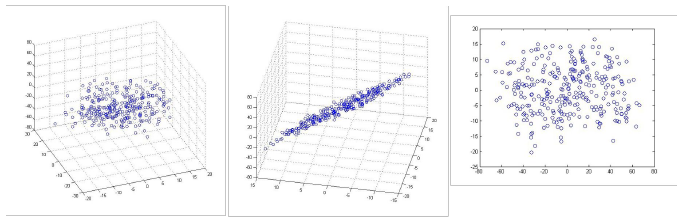
\includegraphics[width=0.6\linewidth]{imgs/chapter12/img0}
	\caption{Idea della dimensionality reduction. Passiamo da 3D a 2D}
	\label{fig:chapter12-00}
\end{figure}

\subsubsection{Varianza lungo una dimensione $\mathbf{w}$}
Per calcolare la varianza lungo una data unit\`a di direzione scegliamo $w$ tale che $w^Tw=1$.
Sia $x_i$ un data point, si necessita di un punto nello spazio $c$ da cui si applica la direzione $w$ per calcolare la varianza di tutti i data points \ref{fig:chapter12-01}:
$$t_i = (x_i-c)^Tw$$


\begin{figure}
	\centering
	\begin{minipage}{.5\textwidth}
		\centering
		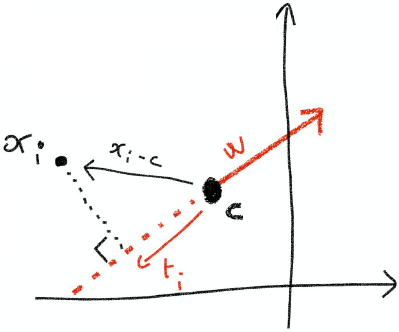
\includegraphics[width=0.6\linewidth]{imgs/chapter12/img1}
		\caption{Varianza lungo una dimensione $\mathbf{w}$}
		\label{fig:chapter12-01}
	\end{minipage}%
	\begin{minipage}{.5\textwidth}
		\centering
		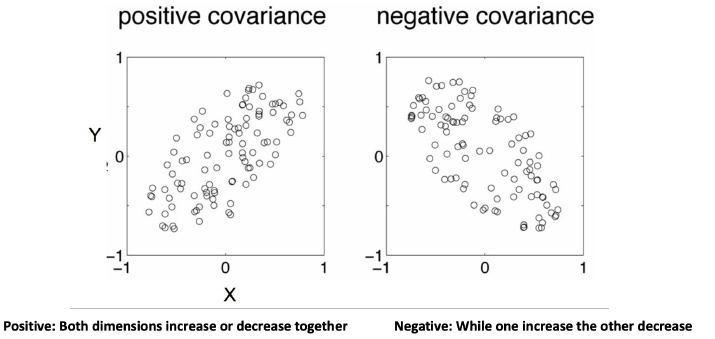
\includegraphics[width=1\linewidth]{imgs/chapter12/img2}
		\caption{Covarianza}
		\label{fig:chapter12-02}
	\end{minipage}
\end{figure}

La proiezione di $x_i$ su $w$.
Il valore atteso $\mathbb{E}[t]$:
\begin{align*}
	\mathbb{E}[t] &= \frac{1}{n}\sum\limits_{i=1}^nt_i = \frac{1}{n}\sum\limits_{i=1}^n(x_i-c)^Tw=\\
	&\bar{x}^Tw-c^Tw
\end{align*}
Ora la varianza sulla dimensione definita da $w$ \`e:
\begin{align*}
	Var[t] &= \frac{1}{n}\sum\limits_{i = 1}^n(t_i -\mathbb{E}[t])^2 = \frac{1}{n}\sum\limits_{i=1}^n[(x_i-\bar{x})^Tw]^2=\\
	&=\frac{1}{n}\sum\limits_{i=1}^n(\bar{x}_i^Tw)^2 = w^T\bigl[\frac{1}{n}\bar{X}\bar{X}^T\bigr]w=\\
	&=w^TCw
\end{align*}
Dove $C$ \`e la matrice della covarianza e $X = [\bar{x}_1,\dots,\bar{x}_n]$.
Si nota come la computazione della varianza non dipende dal punto $c$ in quanto \`e implicitamente calcolata da un punto di vista centrato. La varianza misura la dispersione (spread) dei dati di una determinata variabile intorno alla sua media in una dimensione. La covarianza misura la deviazione dalla media tra due variabili. In altre parole, la covarianza misura la relazione tra due dimensioni. Il segno della covarianza \`e importante: un segno positivo indica una relazione diretta tra le dimensioni confrontate, quindi le due variabili incrementano/decrementano contemporaneamente, un segno negativo indica una relazione indiretta, quindi quando una incrementa l'altra decrementa e viceversa, una correlazione pari a zero indica che non c'\`e relazione tra le dimensioni  \ref{fig:chapter12-02}. Confrontano ogni dimensione con ogni altra andiamo a creare la matrice della covarianza che \`e simmetrica.

\subsubsection{Riassunto eigenvalues e eigenvectors}

Osserva le figure \ref{fig:chapter12-03} e \ref{fig:chapter12-04}.

\begin{figure}
	\centering
	\begin{minipage}{.6\textwidth}
		\centering
		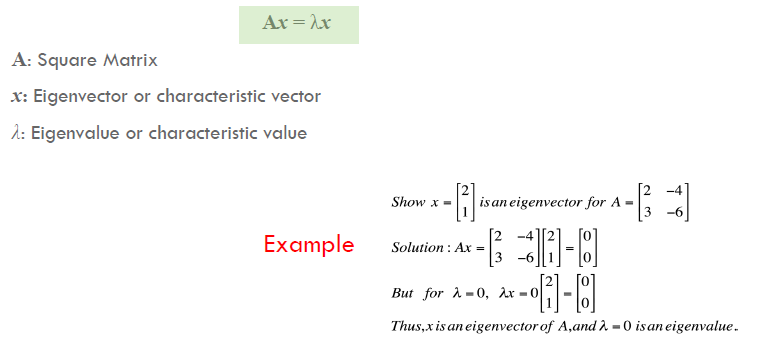
\includegraphics[width=1\linewidth]{imgs/chapter12/img3}
		\caption{}
		\label{fig:chapter12-03}
	\end{minipage}%
	\begin{minipage}{.4\textwidth}
		\centering
		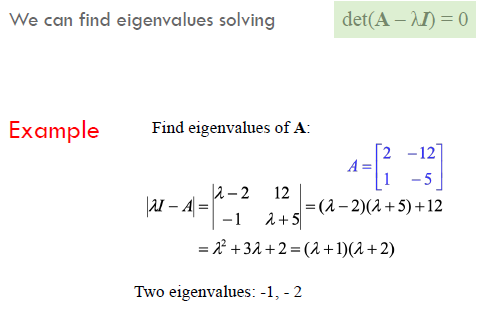
\includegraphics[width=1\linewidth]{imgs/chapter12/img4}
		\caption{}
		\label{fig:chapter12-04}
	\end{minipage}
\end{figure}

\subsubsection{Eigenvalue decomposition}
Sia $A\in R^{m\times m}$ quadrata e simmetrica.
Allora esiste $U=[u_1,\dots,u_n]\in R^{m\times m}$ e $\lambda=(\lambda_1,\dots,\lambda_m)^T\in R^m$ tali che:
$$A = U\Lambda U^T=\sum\limits_{j=1}^m\lambda_ju_ju_j^T$$
E $U^TU=UU^T=I$ e $U$ \`e ortonormale.
Ogni colonna di $U$ ha lunghezza di unit\`a e ogni paio di colonne diverse sono ortogonali tra di loro.
La matrice $\Lambda$ \`e creata con zero da tutte le parti e $\lambda$ sulla diagonale principale.
$u_j$ \`e un eigenvector e $\lambda_j$ \`e la eigenvalue corrispondente.
Si assume un ordinamento discendente: $\lambda_1\ge \lambda_m$.

\subsubsection{First principal component}
Il first principal component \`e la direzione dove la maggior parte della varianza \`e conservata.
Si deve risolvere il problema di massimizzazione della varianza:
$$w_1\in arg\max\{w^TCw:w^Tw=1\}$$
Si devono fare costraints su $w_1$ altrimenti crescerebbero all'infinito.
La varianza di PCA \`e il valore del pi\`u grande eigenvalue della matrice $C$ di covarianza, la prima componente principale \`e il corrispondente vettore $w_1$.
Il maggiore eigenvalue di $C$ \`e la varianza lungo il first principal component e il first principal component $w_1$ \`e il corrispondente eigenvector.

\paragraph{Dimostrazione}
Dalla decomposizione di eigenvalue $C=\sum\limits_j\lambda_ju_ju_j^T$ si assumono le eigenvalue ordinate in ordine discendente.
Allora $W_1^TCw_1 = \sum\limits_j\lambda_j(w_1^Tu_j)^2\le\lambda_1$ in quanto:
$$\sum\limits_j(w_1^Tu_j)^2 = w_1^T\sum\limits_ju_ju_j^Tw_1=w_1^TUU^Tw_1=w_1^Tw_1=1$$
Segue che $\lambda_1\ge w_1^TCw_1 >u_1^TCu_1=\lambda_1$, da cui $w_1^TCw_1=u_1^TCu_1$.
Pertanto $u_1$, l'eigenvector corrispondente al eigenvalue maggiore $\lambda_1$ di $C$ \`e il first principal componente e $\lambda_1$ la varianza lungo di esso.

\subsubsection{Second principal component}
Il second principal component deve essere ortogonale al primo:
$$w_2\in arg\{w^TCw:w^Tw=1,w\perp w_1\}$$
Il secondo eigenvalue maggiore di $C$ \`e la varianza lungo il second principal component e $w_2$ \`e il corrispondente eigenvector.

\paragraph{Dimostrazione}

Dalla decomposizione di eigenvalue $C=\sum\limits_j\lambda_ju_ju_j^T$ si assumono le eigenvalue ordinate in ordine discendente.
Allora
$$W_2^TCw_2 = \sum\limits_{j=1}^m\lambda_j(w_2^Tu_j)^2=\lambda_1w_2^Tu_1+\sum\limits_{j=2}^m\lambda_j(w_2^Tu_j)^2\le\lambda_2$$
In quanto:
$$\sum\limits_j(w_2^Tu_j)^2 = w_2^T\sum\limits_ju_ju_j^Tw_2=w_2^TUU^Tw_2=w_2^Tw_2=1$$
Segue che $\lambda_2\ge w_2^TCw_2 >u_2^TCu_2=\lambda_2$, da cui $w_2^TCw_2=u_2^TCu_2$.
Pertanto $u_2$, l'eigenvector corrispondente al secondo eigenvalue maggiore $\lambda_2$ di $C$ \`e il second principal componente e $\lambda_2$ la varianza lungo di esso.

\subsubsection{Iesimo principal component}
Allo stesso modo:
$$w_i\in arg\{w^TCw:w^Tw=1,w\perp w_j 1\le j < i\}$$
L'i-esimo eigenvalue maggiore di $C$ \`e la varianza lungo l'iesimo principal component.
L'iesimo principal component \`e $w_i$ \`e il corrispondente eigenvector.
La dimostrazione \`e analoga a quella del second principal component.

\subsubsection{PCA utilizzando eigenvalue decomposition}
\begin{itemize}
	\item Siano i data points $X=[x_1,\dots,x_n]$.
	\item Si centri $\bar{X} = X-\frac{1}{n}X1_n1_n^T$.
	\item Si computi la matrice di covarianza $C=\frac{1}{n}\bar{X}\bar{X}^T$.
	\item Eigenvalue decomposition: $U,\lambda = eig(C)$.
	\item Principal components: $W=U=[u_1,\dots,u_m]$, varianze $\lambda = (\lambda_1,\dots,\lambda_m)$.
\end{itemize}

\subsubsection{PCA utilizzando singular value decomposition (SVD)}
Sia $A\in\mathbb{R}^{m\times n}$.
Allora esiste $U\in\mathbb{R}^{m\times k}$, $s\in\mathbb{R}^k$ con $s_1\ge\cdots\ge s_K >0$ e $V\in \mathbb{R}^{n\times k}$ tali che:
$$A = USV^T\qquad\qquad\land\qquad\qquad U^TU=V^TV=I$$
Si computa pertanto la SVD di $\bar{X}:U,s,V=SVD(\bar{X})$.
Le componenti principali $U=[u_1,\dots,u_k]$ e le varianze $\bigl(\frac{s_1^2}{n},\dots,\frac{s_k^2}{n}\bigr)$
La matrice $U$ \`e la matrice con gli eigenvectors.
Le eigenvalue possono essere calcolate in quanto: $\bar{x} = USV^T$ e $c = \frac{1}{n}\bar{x}\bar{x}^T = \frac{1}{n}USV^TVSU^T=U\frac{s^2}{n}u^T$

\subsubsection{Dimensionality reduction}
Sia $\hat{W} = [w_1,\dots,w_k]$ le prime $k$ componenti principali derivate dai data points $\bar{X} = [\bar{x}_1,\dots,\bar{x}_n]$.
Si cambia a un sistema di coordinate ridotto con le $k$ componenti principali con $\hat{W}$ come assi:
$$T = \hat{W}^T\bar{X}\in\mathbb{R}^{k\times n}$$
Dove $T$ \`e il principal component scores.
Si pu\`o usare la eigenvalue decomposition o SVD per computare la decomposizione completa.
Con la PCA si ottengono gli eigenvectors o componenti, si possono ordinare e usarli per comporre la matrice $\hat{W}$.
Una volta fatto quello si usa per calcolare $T$ che \`e il dataset dimensionalmente ridotto.

\subsubsection{Interpretazioni alternative}
Si pu\`o considerare la first principal component come la linea nello spazio con la minore distanza quadrata dai data points.
La stessa interpretazione pu\`o essere data alle altre componenti principali.

\subsubsection{Scalare delle variabili}
PCA \`e sensibile alla scala delle features, pertanto \`e raccomandato scalarle secondo la standard deviation.

\subsubsection{Esempio}

Per un esempio osserva le figure \ref{fig:chapter12-05}, \ref{fig:chapter12-06}, \ref{fig:chapter12-07}, \ref{fig:chapter12-08} e \ref{fig:chapter12-09}.


\begin{figure}
	\centering
	\begin{minipage}{.5\textwidth}
		\centering
		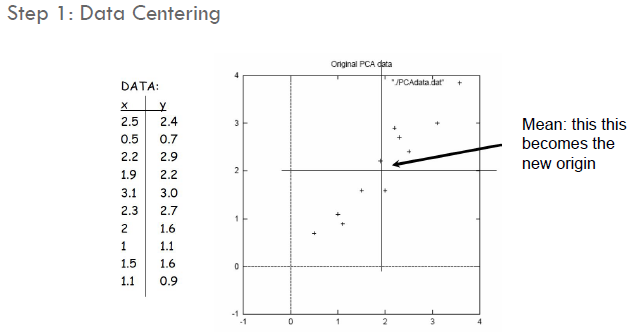
\includegraphics[width=1\linewidth]{imgs/chapter12/img5}
		\caption{}
		\label{fig:chapter12-05}
	\end{minipage}%
	\begin{minipage}{.5\textwidth}
		\centering
		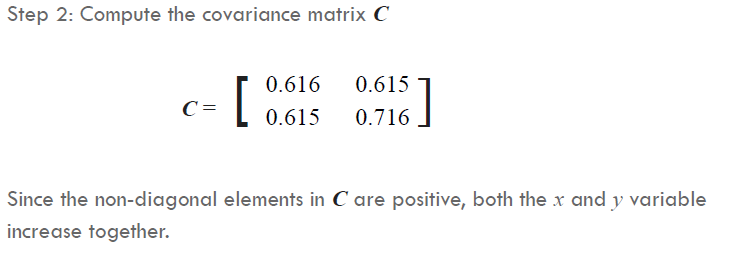
\includegraphics[width=1\linewidth]{imgs/chapter12/img6}
		\caption{}
		\label{fig:chapter12-06}
	\end{minipage}
\end{figure}

\begin{figure}
	\centering
	\begin{minipage}{.5\textwidth}
		\centering
		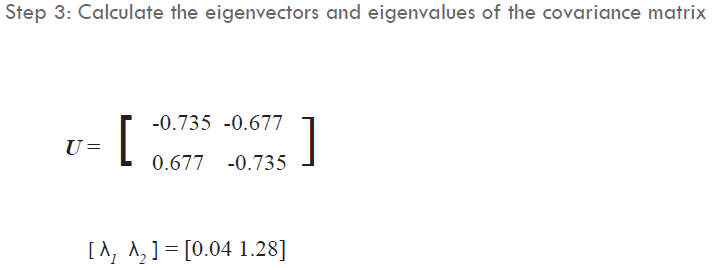
\includegraphics[width=1\linewidth]{imgs/chapter12/img7}
		\caption{}
		\label{fig:chapter12-07}
	\end{minipage}%
	\begin{minipage}{.5\textwidth}
		\centering
		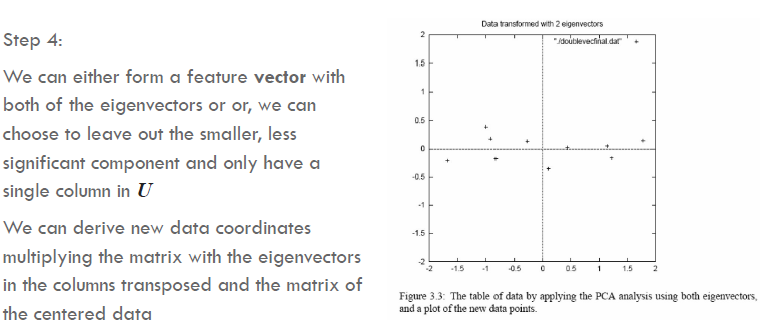
\includegraphics[width=1\linewidth]{imgs/chapter12/img8}
		\caption{}
		\label{fig:chapter12-08}
	\end{minipage}
\end{figure}

\begin{figure}
	\centering
	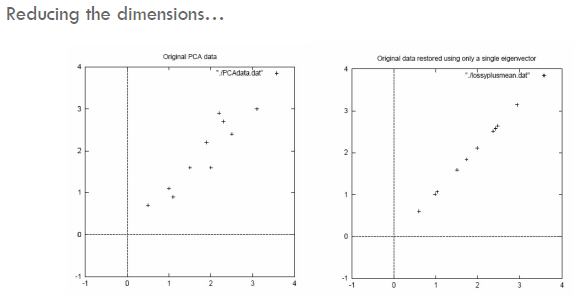
\includegraphics[width=0.6\linewidth]{imgs/chapter12/img9}
	\caption{}
	\label{fig:chapter12-09}
\end{figure}

\subsubsection{Componenti principali da considerare}
Il numero di componenti per la dimensionality reduction dipende dall'obiettivo e dall'applicazione.
Non ci sono modi per validarla a meno di volerla usare in un contesto di un modello con supervision, ma si pu\`o calcolare la proporzione cumulativa di varianza spiegata che per i primi principal component \`e:
$$\frac{\sum\limits_{j = 1}^k\lambda_j}{\sum\limits_{j = 1}^m C_{jj}}$$
A parole: stiamo riducendo da m a k dimensioni, se il risultato \`e alto, per esempio 0.99 significa che riducendo da m a k dimensioni siamo comunque in grado di spiegare bene di dati, un numero pi\`u basso indica che stiamo perdendo troppe informazioni.
Per la eigenvalue decomposition \`e:
$$\frac{\sum\limits_{j = 1}^ks^2_j}{\sum\limits_{ij} \bar{X}^2C_{ji}}$$
Queste formule permettono di stimare la quantit\`a di informazione persa calcolando la percentuale di varianza che si \`e mantenuta riducendo la dimensionalit\`a dei dati.

\subsubsection{Kernel PCA}
La PCA riduce la dimensionalit\`a attraverso una trasformazione lineare.
Pertanto utilizzando il kernel trick si pu\`o applicare una PCA in uno spazio a pi\`u dimensioni ottenendo una trasformazione non lineare nello spazio originale \ref{fig:chapter12-10}.
\begin{figure}
	\centering
	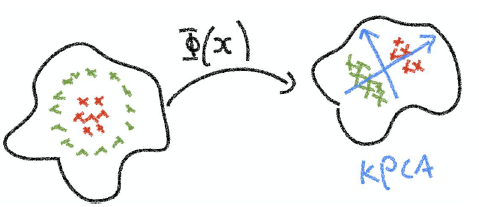
\includegraphics[width=0.6\linewidth]{imgs/chapter12/img10}
	\caption{Kernel PCA. La funzione sar\`a calcolata implicitamente utilizzando il kernel}
	\label{fig:chapter12-10}
\end{figure}
\section{Altre tecniche di dimensionality reduction}
\begin{itemize}
	\item PCA (Principal Component Analysis): Trova la proiezione che massimizza la varianza
	\item Multidimensional Scaling: Trovare la proiezione che meglio preserva le distanze interpunto distanze tra i punti 
	\item LDA (Linear Discriminant Analysis): Massimizzazione degli assi delle componenti per separazione delle classi
\end{itemize}

\section{Applicazioni del PCA}
Come detto in precedenza la PCA pu\`o essere utilizzata per risolvere il problema del riconoscimento facciale. Tratteremo i pixel delle immagini come vettori e andremo in fine a cercare l'immagine pi\`u simile con una ricerca nearest-neighbor. Le immagini di per se sono estremamente di alte dimensioni, con immagini di 100x100 pixel si raggiungono dimensioni nelle decine di centinaia di valori per ogni immagine, ma solo pochi vettori di 10000 dimensioni sono immagini valide. Possiamo trovare il migliore sottospazio dei vettori di 10000 dimensioni dove i vettori sono immagini di facce.

\section{Clustering}
\subsection{Task}
Si deve trovare una funzione $f\in N^X$ che assegna ogni input $x\in X$ a un indice di cluster $f(x)\in N$.
Tutti i punti mappati allo stesso indice formano un cluster.
Ci sono diversi tipi di cluster: partizionali, gerarchici e overlapped.
Permette di trovare gruppi di dati con delle propriet\`a interne, comprimere i dati riducendo il numero di data points invece di ridurre la dimensionalit\`a delle features.	

\subsection{K-means clustering}
Il K-means clustering richiede di sapere prima il numero $k$ di gruppi in cui si vogliono dividere i dati.
Siano i data points $X=[x_1,\dots,x_n]\in\mathbb{R}^{d\times n}$.
Fissato un numero di cluster $k$, si vuole trovare una partizione di data points in $k$ insiemi $\mathcal{L}_1,\dots,\mathcal{L}_k$ che minimizza la variazione $V(\mathcal{L}_j)$ in ogni set $\mathcal{L}_j$
$$\min\limits_{\mathcal{L}_1,\dots,\mathcal{L}_K}\sum\limits_{j = 1}^kV(\mathcal{L}_j)$$
La variazione \`e tipicamente data da $V(\mathcal{L}_j) = \sum\limits_{i\in\mathcal{L}_j}||x_i-\mu_j||^2$, dove $\mu_j = \frac{1}{|\mathcal{L}_j|}\sum\limits_{i\in\mathcal{L}_j}x_i$, il centroide di $\mathcal{L}_j$.
Si deve definire una funzione obiettivo che minimizza la somma di variazioni in ogni set creato.
L'algoritmo di ottimizzazione \`e semplice, inizializza con centroidi casuali e poi mentre i cluster cambiano assegna ogni datapoint al centroide pi\`u vicino formando nuovi cluster e computando nuovi centroidi \ref{fig:chapter12-11}.
\begin{figure}
	\centering
	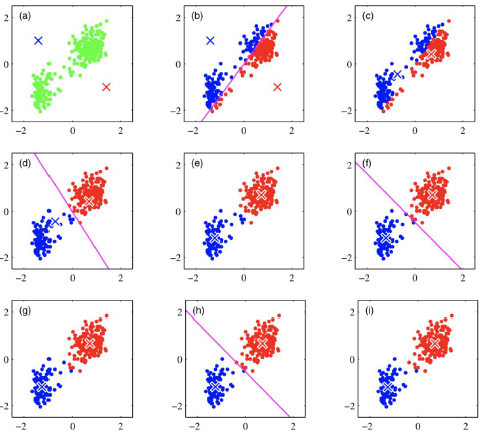
\includegraphics[width=0.6\linewidth]{imgs/chapter12/img11}
	\caption{Esempio. Partiamo da due punti casuali e poi raffiniamo le scelte}
	\label{fig:chapter12-11}
\end{figure}

Questo algoritmo ha una convergenza garantita in quanto migliora strettamente la assignment di cluster e siccome sono finiti a un certo punto converge per forza.
Non \`e comunque garantito trovi il minimo in quanto \`e un problema NP-hard anche sul piano, troveremo un minimo locale.
\`E sensibile alla scala delle features: in alcuni casi avremo bisogno di una funzione di normalizzazione delle features.

\subsubsection{Distanza}
La distanza euclidea:
$$d(x,y) = \sqrt{\sum\limits_{i=1}^n(x_i-y_i)^2}$$
Non \`e sempre una buona scelta: per esempio, nel fare clustering di documenti si sceglie una feature per ogni parola e il valore \`e il numero di volte che tale parola compare.
Si nota come qui due distribuzioni possono avere una grande distanza ma distribuzioni simili.

\paragraph{Cosine similarity}
Per risolvere questo problema si utilizza la cosine similarity:
$$sim(x,y) = \frac{x\cdot y}{|x||y|} = \frac{x}{|x|}\cdot\frac{y}{|y|} = \frac{\sum\limits_{i = 1}^n x_iy_i}{\sqrt{\sum\limits_{i = 1}^n x_i^2}\sqrt{\sum\limits_{i = 1}^ny_i^2}}$$
Questa \`e correlata con l'angolo tra due vettori.
Varia tra $0$ e $1$.
\`E buona per dati di testo e molti altri.
Di facile computazione in quanto si possono considerare solo features con valori non zero in entrambi gli esempi.
La cosine distance:
$$d(x,y) = 1-sim(x,y)$$

\subsubsection{Propriet\`a di K-means}

\paragraph{Convergenza}
L'algoritmo \`e garantito che converga in quanto migliora strettamente l'obiettivo se c'\`e almeno un cambio di cluster e l'insieme delle partizioni \`e finito.
Questo avviene in quanto durante il primo step di assignment ogni altro assignment causerebbe una loss maggiore e durante la computazione del centroide la media di un insieme di valori minimizza l'errore quadratico.

\paragraph{Minimo}
Non \`e garantito che trovi il minimo globale ma uno locale.
Questo avviene in quanto tipicamente la loss function \`e non convessa.

\paragraph{Selezione dei centroidi}
I risultati possono variare enormemente sulla scelta dei centroidi con random seed selection: alcuni possono causare povera convergenza o convergenza a cluster sub-ottimali.
Alcune euristiche comuni sono:
\begin{multicols}{2}
	\begin{itemize}
		\item Punti casuali nello spazio.
		\item Esempi scelti casualmente.
		\item Punti meno simili a ogni centro esistente.
		\item Si provano diversi punti di inizio.
		\item Si inizializza con i risultati di un altro metodo di clustering.
	\end{itemize}
\end{multicols}

\subsection{Problematiche del clustering}
Il clustering presenta diverse problematiche:
\begin{multicols}{2}
	\begin{itemize}
		\item Rappresentazione di un esempio per il cluster.
		\item Simiglianza e distanza tra esempi.
		\item Clustering piatto o gerarchico.
		\item Numero di cluster fisso o data driven.
	\end{itemize}
\end{multicols}

\subsection{Algoritmi di clustering}

\subsubsection{Flat algorithms}
Tipicamente iniziano con un partizionamento causale parziale che viene raffinato iterativamente.
Sono per esempio K means, model based e spectral.

\subsubsection{Hierarchical algorithms}
Si dividono in agglomerativi bottom-up o divisivi top-down.

\subsubsection{Hard clustering}
Nell'hard clustering ogni esempio appartiene esattamente ad un cluster.

\subsubsection{Soft clustering}
Nel soft clustering ogni esempio pu\`o appartenere a pi\`u di un cluster.
\`E pertanto probalistico.

\subsection{EM clustering}
Si nota come il K-means clustering assume sempre dei cluster circolari.
Per questo EM clustering assume che i dati vengano da un'insieme di gaussiane: sono cos\`i ellittici.
Ogni dato viene assegnato a un cluster con una certa probabilit\`a: soft clustering.
\`E molto simile a un alto livello a K-means: itera tra assigning points e ricalcolando i centri dei cluster.
Le differenze principali sono che si assumano cluster ellittici e che sia un algoritmo di soft-clustering.
Pertanto si inizia con dei centri di cluster iniziale, successivamente si assegnano soft points ad ogni cluster calcolando $p(\theta_c|x)$ la probabilit\`a che ognuno di essi appartenga a un cluster \ref{fig:chapter12-12}.
Si ricalcolano i centri del cluster con nuovi parametri $\theta_c$, la massima probabilit\`a dei centri dati il corrente soft clustering.
I centri ottengono una contribuzione pesata dai punti.
\begin{figure}
	\centering
	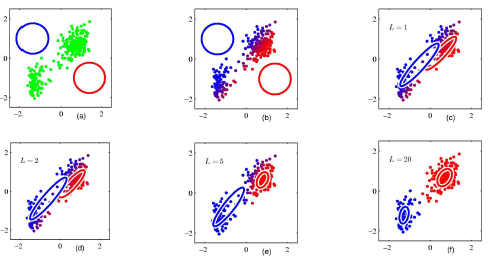
\includegraphics[width=0.8\linewidth]{imgs/chapter12/img12}
	\caption{Esempio}
	\label{fig:chapter12-12}
\end{figure}

\subsubsection{Mixture of Gaussians}
In una dimensione una gaussiana:
$$f(x;\sigma;\mu) = \frac{1}{\sigma\sqrt{2\pi}}e^{-\frac{(x-\mu)^2}{2\sigma^2}}$$
In $m$ dimensioni invece:
$$N[x;\mu;\Sigma] = \frac{1}{(2\pi)^{\frac{d}{2}}\sqrt{det(\Sigma)}}e^{[-\frac{1}{2}(x-\mu)^T\Sigma^{-1}(x-\mu)]}$$
Si impara pertanto la media di ogni cluster o suo centro e la matrice di covarianza, ovvero quanto si disperde, la forma del contorno.

\subsubsection{Soft cluster points}
Si assegna soft ogni punto a ogni cluster calcolando $p(\theta_c|x)$ o la probabilit\`a di ogni punto di appartenere al cluster.
Si utilizza l'equazione della Gaussiana per ogni cluster normalizzata per creare una probabilit\`a.

\subsubsection{Ricalcolo dei centri}
Si calcolano nuovi parametri di cluster $\theta_c$.
Il maximum likelihood cluster center dati il soft clustering corrente.
Questo si fa fittando una gaussiana.

\paragraph{Fit di una gaussiana}
Si fa calcolando la media $\mu$ e la varianza $\sigma$ dei dati.

\subsubsection{Conclusione}
EM clustering sta per expectation maximization.
Per expectation si intende dato il modello corrente, si trova le probabilit\`a aspettate dei data points ad ogni cluster.
La massimizzazione \`e dato l'assignment probabilistico di tutti i punti la stima del nuovo modello $\theta_c$.
Come $k$-means \`e garantito che converga ad un ottimo locale, \`e un algoritmo general purpose per fare training di un modello senza labels.

\subsection{Altri algoritmi di clustering}
K-means e EM-clustering non possono gestire tutte le task di clustering.
In particolare non possono gestire dati non distribuiti secondo una gaussiana, soffrono dello stesso problema dei modelli lineari in quanto non sono in grado di prendere decisioni locali.

\subsubsection{Spectral clustering}
Nello spectral clustering avviene una partizione a grafo: si definisce una matrice di somiglianza e si taglia il grafo.

\subsubsection{Clustering gerarchico}
Il clustering gerarchico produce un insieme di cluster nested organizzati come un albero gerarchico detto dendrogram.
Viene tipicamente utilizzato per i profili genici.

\section{Density estimation}

\subsection{Task}
Si deve trovare una distribuzione di probabilit\`a $f\in \Delta(X)$ che fitta i dati $x\in X$.
Permette di ritornare una stima esplicita della distribuzione di probabilit\`a che genera i dati.
Permette la generazione di nuovi dati dalla stessa distribuzione e l'individuazione di anomalie.

\subsection{Generative model}
I generative model risolvono la task della density estimation.
Sono modelli statistici della distribuzione dei dati sull'input $p_x$ o di una joint distribution sulla coppia di input label $p_{XY}$ dipendente dalla disponibilit\`a dei dati obiettivo.
La loro abilit\`a principale \`e di generare nuovi dati dalle distribuzioni osservate. Immagine di aver allenato un modello fornendo una grande quantit'a di immagini di gatti, ad un certo punto il modello avr'a imparato cosa rende un gatto, un gatto, per esempio la forma, il colore, e dato in input un immagine con solo rumore casuale, generare un gatto simile a quelli visti in precedenza.

\subsection{Modelli discriminativi}
I modelli discriminativi sono modelli statistici della distribuzione di probabilit\`a condizionale $p_{Y|X}$ del target dato l'input.
Tipicamente svolgono una task di classificazione come SVM, decision trees e classificatori KNN. Un esempio \`e un modello in grado di distinguere immagini di cani e gatti e data un'immagine il modello fornisce una confidenza che nella data immagine sia rappresentato un cane o un gatto.
Un modello discriminativo pu\`o essere costruito da uno generativo attraverso la regola di Bayes ma non viceversa:
$$p_{Y|X}(x) = \dfrac{p_{XY}(x,y)}{\sum\limits_{y'}p_{XY}(x,y')p_X(x)}$$

\subsection{Tipi di density estimation}
Per entrambi i modi si trovano due tipi della task:
\begin{itemize}
	\item Supervised: $Z\in X\times Y$.
	\item Unsupervised $Z\in X$.
\end{itemize}

\subsubsection{Explicit density estimation}
Si deve trovare una distribuzione di probabilit\`a $f\in \Delta(Z)$ che fitta i dati $z\in Z$ dove $z$ \`e campionato da una distribuzione di dati sconosciuta $p_{data}\in\Delta(Z)$ \ref{fig:chapter12-18}.

\subsubsection{Implicit density estimation}
Si vuole trovare una funzione $f\in Z^\Omega$ che genera i dati $f(\omega)\in Z$ da un input $\omega$ campionato da una distribuzione predefinita $p_\omega\in\Delta(\Omega)$ in modo che la distribuzione del campione generato fitta la distribuzione sconosciuta $p_{data}\in\Delta(Z)$.
Non si stima la probabilit\`a $\omega$ ma ci si concentra unicamente sul riprodurre i dati con la stessa distribuzione di quella sconosciuta originaria \ref{fig:chapter12-19}.

\begin{figure}
	\centering
	\begin{minipage}{.5\textwidth}
		\centering
		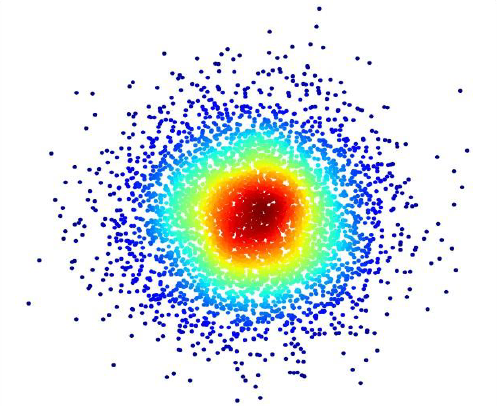
\includegraphics[width=0.7\linewidth]{imgs/chapter12/img18}
		\caption{Explicit density estimation}
		\label{fig:chapter12-18}
	\end{minipage}%
	\begin{minipage}{.5\textwidth}
		\centering
		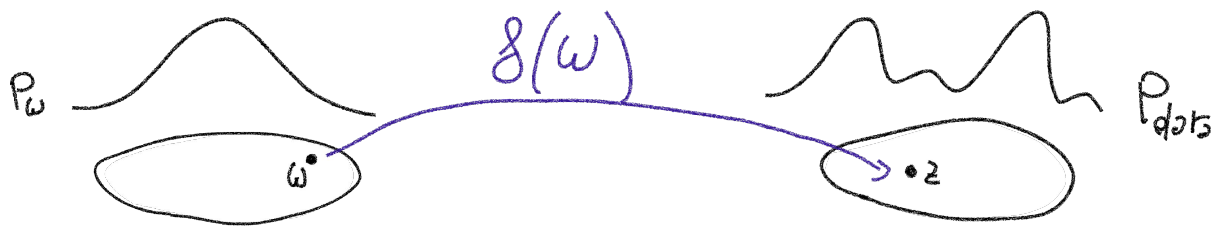
\includegraphics[width=1\linewidth]{imgs/chapter12/img19}
		\caption{Implicit density estimation}
		\label{fig:chapter12-19}
	\end{minipage}
\end{figure}


\subsubsection{Obiettivo per i modelli generativi}
Si deve definire uno spazio di ipotesi $H\subset \Delta(Z)$, consiste di un insieme di modelli che possono rappresentare distribuzioni di probabilit\`a definite esplicitamente o implicitamente.
Si definisce una misura di divergenza $d\in R_+^{\Delta(Z)\times\Delta(Z)}$ tra le distribuzione di probabilit\`a in $\Delta(Z)$ e si usa la divergenza di Kullback-Leibler.
La divergenza \`e $0$ se due distribuzioni hanno un match, altrimenti \`e negativa.
L'algoritmo tenta di trovare $q^*\in H$ che ha un fit migliore sui dati distribuiti secondo $p_{data}$ dove il best fit \`e quello con la divergenza minore.
$$q^*\in arg\min\limits_{q\in\mathcal{H}}d(p_{data},q)$$
Si assumer\`a che la distribuzione dei dati \`e solo su $X$ con unsupervised learning, ma il trasporto a supervised \`e banale.

\subsection{Variational AutoEncoder (VAE)}
Un autoencoder \`e un modo per comprimere dati ad alta dimensione in una rappresentazione a meno dimensioni: dimensionality reduction.
Un encoder mappa i dati di input $x$ a una rappresentazione compressa $\omega$.
La rappresentazione conserva fattori significativi nella variazione dei dati come in PCA.

\subsubsection{Training}
Un encoder viene trainato creando un decoder che mappa la rappresentazione di $\omega$ indietro nel dominio di input portando a una ricostruzione $\hat{x}$.
Pertanto l'encoder autoencoda il proprio input.
L'obiettivo \`e quello di minimizzare la divergenza tra l'input $x$ e la sua ricostruzione $\hat{x}$ che porta all'algoritmo di training verso la minima perdita di informazione durante la fase di encoding.
Dopo il training il decoder non \`e pi\`u necessario in quanto \`e funzionale solo per stimare l'encoder.
L'encoder invece pu\`o essere utile per diverse tasks, per esempio per inizializzare o precomputare le caratteristiche per supervised models.

\subsubsection{Generare dati con il decoder}
Il decoder potrebbe essere usato per generare nuovi dati ma non li generer\`a secondo $p_{data}$ in quanto niente lo obbliga.
Se si genera un input a caso $\omega$ non si \`e sicuri che $\omega$ \`e una combinazione che verrebbe ordinata dalla distribuzione dei dati.
La soluzione a questo problema sarebbe di avere una distribuzione a priori $\Omega$ che ci dice la probabilit\`a di campionare ogni $\omega$ dallo spazio encodato.
Il decoder poi sarebbe capace di tradurre la distribuzione $\Omega$ nella distribuzione di dati in $X$ \ref{fig:chapter12-13}.
\begin{figure}
	\centering
	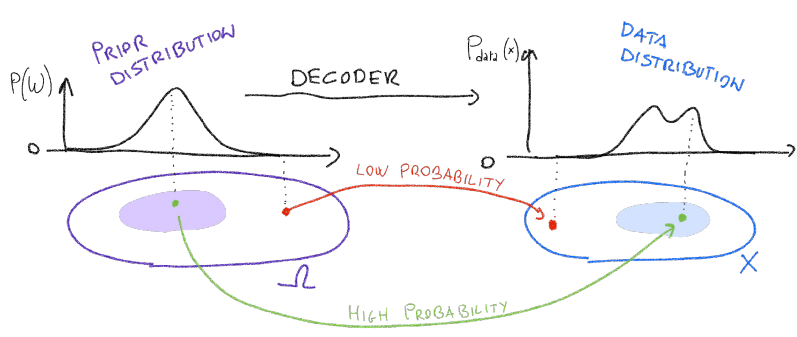
\includegraphics[width=0.6\linewidth]{imgs/chapter12/img13}
	\caption{Cosa vorremmo}
	\label{fig:chapter12-13}
\end{figure}

\paragraph{Training del decoder}
In termini formali il decoder: $q_\theta(x|\omega)$ \`e una distribuzione di probabilit\`a $x$ per ogni valore $\omega$.
La probabilit\`a a priori \`e $p_\omega$
Si pu\`o ottenere un'aspettativa marginalizzata
$$q_\theta(x) = \mathbb{E}_{\omega\sim p_\omega}[q_\theta(x|\omega)]$$
Successivamente si pone come obiettivo modificare il parametro $\theta$ per minimizzare la divergenza tra la distribuzione dei dati e $q_\theta$:
$$\theta^*\in arg\min\limits_{\theta\in\Theta}d(q_\theta,p_{data})$$
Si utilizza KL-divergence.
\`E non negativa e $0$ se $p$ e $q$ sono la stessa distribuzione.
$$d_{KL}(p,q) = \mathbb{E}_{x\sim p}\bigl[\log\frac{p(x)}{q(x)}\bigr]$$

\paragraph{Intrattabilit\`a}
Analizzando la divergenza si vede che il suo calcolo \`e intrattabile a causa del valore atteso:
\begin{align*}
	d_{KL}(p_{data}, q_\theta) &= \mathbb{E}_{x\sim p_{data}}\bigl[\log\frac{p_{data}(x)}{q_\theta(x)}\bigr]=\\
	& = -\mathbb{E}_{x\sim p_{data}}[\log q_\theta(x)] + const=\\
	&= -\mathbb{E}_{x\sim p_{data}}[\log\mathbb{E}_{\omega\sim p_\omega} [q_\theta(x|\omega)]]+const
\end{align*}
Si pu\`o approssimare il valore atteso attraverso stochastic gradient descent.
\begin{align*}
	\frac{d}{d\theta}d_{KL}(p_{data},q_\theta) &= -\frac{d}{d\theta}\mathbb{E}_{x\sim p_{data}}[\log\mathbb{E}_{\omega\sim p_\omega}[q_\theta(x|\omega)]=\\
	& = -\mathbb{E}_{x\sim p_{data}}\bigl[\frac{d}{d\theta}\log\mathbb{E}_{\omega\sim p_\omega}[q_\theta(x|\omega)]\bigr]=\\
	& = - \mathbb{E}_{x\sim p_{data}}\biggl[\dfrac{\frac{d}{d\theta}\mathbb{E}_{\omega\sim p_\omega}[q_\theta(x|\omega)]}{\mathbb{E}_{\omega\sim p_\omega}[q_\theta(x|\omega)]}\biggr]=\\
	& = - \mathbb{E}_{x\sim p_{data}}\mathbb{E}_{\omega\sim p_\omega}\biggl[\dfrac{\frac{d}{d\theta}q_\theta(x|\omega)}{\mathbb{E}_{\omega\sim p_\omega}[q_\theta(x|\omega)]}\biggr]
\end{align*}
Queste stime sono comunque dipendenti da $\omega$ e questo le rende biased e ancora intrattabili.

\paragraph{Variational bound}
Si introduce pertanto un nuovo termine $q_\psi(x)\in\Delta(\Omega)$.
Viene usato per calcolare due termini: un recostruction term e un regolarizzatore.
Ora in particolare si nota come:
\begin{align*}
	\log\mathbb{E}_{\omega\sim p_\omega} [q_\theta(x|\omega)] &= \log\mathbb{E}_{\omega\sim q_\psi(\cdot|x)}\bigl[q_\theta(x|\omega)\frac{p_w(w)}{q_\psi(\omega|x)}\bigr]\ge\\
	&\ge \mathbb{E}_{\omega\sim q_\psi(\cdot|x)}\bigl[\log\bigl(q_\theta(x|\omega)\frac{p_\omega(\omega)}{q_\psi(\omega|x)}\bigr)\bigr]=\\
	&=\mathbb{E}_{\omega\sim q_\psi(\cdot|x)}[\log q_\theta(x|\omega)] - d_{KL}(q_\psi(\omega|x), p_w)
\end{align*}
Dove il primo termine della sottrazione \`e il ricostruttore e il secondo il regolarizzatore.
Si nota come il ricostrutture \`e ancora di intrattabile computazione ma pu\`o essere facile ottenere delle stime del gradiente non biased con rispetto di $\theta$ e $\psi$.
Il regolarizzatore pu\`o avere una soluzione con forma chiusa utilizzando una distribuzione gaussiana.

\paragraph{Training in pratica}
Viene campionato un sample $x$ da $p_{data}$.
Questo viene passato dal encoder $q_\psi$ che produce una media $\mu_{\omega|x}$ e una covarianza $\Sigma_{\omega|x}$ utilizzati per costruire una gaussiana utilizzata per costruire il regularization term e il sample $\omega$.
$\omega$ \`e l'input del decoder $q_\theta$ che produce una media $\mu_{x|\omega}$ e una covarianza $\Sigma_{x|\omega}$, utilizzati per costruire una gaussiana, che insieme ad $x$ costruisce il reconstruction term.
Il reconstruction e il regularization term vengono usati per computare il variational lower bound loss, con il secondo come $P_\omega = N(0,1)$, di normale standard e questo viene usato per aggiornare $\theta$ e $\psi$ \ref{fig:chapter12-14}.

\begin{figure}
	\centering
	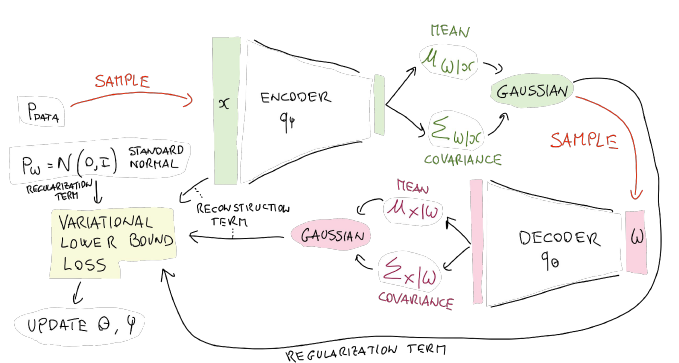
\includegraphics[width=0.8\linewidth]{imgs/chapter12/img14}
	\caption{Training in pratica}
	\label{fig:chapter12-14}
\end{figure}
\subsubsection{VAE condizionale}
Si assuma di avere un informazione $y\in\mathcal{Y}$ e si vuole generare nuovi dati sull'informazione.
Denota una distribuzione si probabilit\`a di encoding.
Si modifica il encoder e il decoder per prendere le informazioni in input ottenendo
$$q_\phi(\omega|x,y)$$
$$q_\theta(\omega|x,y)$$
Si definisce i priori condizionati sull'informazione $p_\omega(\omega|y)$.
Le VAE condizionali sono usate per direzionare l'output che si vuole dal generative model, altrimenti l'output seguirebbe solo la distribuzione di probabilit\`a dei dati. Esempio: dato un viso, generare il viso con occhiali.

\subsubsection{Probabilit\`a dei VAE}
\begin{itemize}
	\item Underfitting: agli stage iniziali il regolarizzatore \`e troppo forte e tende ad annullare la capacit\`a del modello.
	\item Blurry samples: il generatore tende a produrre data blurry in quanto la gaussiana tende a produrre blurry risultati.
\end{itemize}

\subsection{Generative adversarial Networks (GAN)}
Le GAN permettono di stimare la densit\`a implicitamente.
Si assuma di avere una densit\`a a priori $p_\omega\in\Delta(\Omega)$ e un generatore o decoder $g_\theta\in X^\Omega$ che genera i data points in $X$ dato un random point da $\Omega$ \ref{fig:chapter12-15}.
\begin{figure}
	\centering
	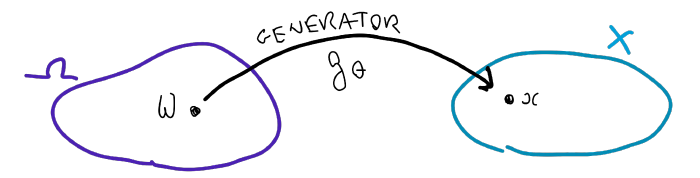
\includegraphics[width=0.6\linewidth]{imgs/chapter12/img15}
	\caption{Generative Adversarial Networks (GAN)}
	\label{fig:chapter12-15}
\end{figure}
Il generatore campiona direttametne dalla distribuzione implicita che non si conosce.
La densit\`a \`e indotta da $p_\omega$ e il generatore $g_\theta$ \`e dato da $q_\theta(x) = \mathbb{E}_{\omega\sim p_\omega}\delta[g_\theta(\omega) - x]$ dove $\delta$ \`e la funzione delta di Dirac.
L'obiettivo di GAN \`e trovare $\theta^*$ tale che $q_{\theta^*}$ che fitta meglio la distribuzione $p_{data}$ sotto la divergenza di Jensen-Shannon $d_{jS}$:
$$\theta^*\in arg\min\limits_{\theta} d_{JS}(p_{data},q_\theta)$$
Dove:
$$d_{JS}(p,q) = \frac{1}{2}d_{KL}\bigl(p,\frac{p+q}{2}\bigr)+\frac{1}{2}d_{KL}\bigl(q,\frac{p+q}{2}\bigr)$$
Che \`e chiaramente intrattabile da computare in quanto richiama la convergenza $KL$.
Lo stesso vale per il gradiente.

\subsubsection{Forma equivalente della divergenza JS}
\begin{align*}
	d_{JS}(p,q) &= \frac{1}{2}d_{KL}\bigl(p, \frac{p+q}{2}\bigr) + \frac{1}{2}d_{KL}\bigl(q, \frac{p+q}{2}\bigr)=\\
	&=\frac{1}{2}\mathbb{E}_{x\sim p}\bigl[\log\frac{2p(x)}{p(x)+q(x)}]\bigr]+\frac{1}{2}\mathbb{E}_{x\sim q}\bigl[\log\frac{2q(x)}{p(x)+q(x)}\bigr]=\\
	&=\frac{1}{2}\mathbb{E}_{x\sim p}\bigl[\log\frac{p(x)}{p(x)+q(x)}]\bigr]+\frac{1}{2}\mathbb{E}_{x\sim q}\bigl[\log\frac{q(x)}{p(x)+q(x)}\bigr] + \log(2)=\\
	&=\log(2)+\frac{1}{2}\max\limits_t\{\mathbb{E}_{x\sim p}[\log t(x)]+\mathbb{E}_{x\sim q}[\log(1-t(x))]\}
\end{align*}
Si deve pertanto imparare $t(x)$, un binary classifier che predice se $x$ deriva da $p$ o $q$.

\subsubsection{Obiettivo della GAN}
Sia $t_\varphi$ un classificatore o discriminatore per i data points in $\mathcal{X}$.
Allora si trova il limite inferiore sull'obiettivo:
\begin{align*}
	d_{JS}(p_{data}, q_\theta) &= \log(2) + \frac{1}{2}\max\limits_t\{\mathbb{E}_{x\sim p_{data}}[\log t(x)] + \mathbb{E}_{x\sim q_\theta}[\log(1-t(x))]\}\ge\\
	&= \log(2) + \frac{1}{2}\max\limits_\varphi\{\mathbb{E}_{x\sim p_{data}}[\log t_\varphi(x)] + \mathbb{E}_{x\sim q_\theta}[\log(1-t_\varphi(x))]\}
\end{align*}
Si possono ignorare $\frac{1}{2}$ e $\log(2)$ in quanto non cambiano il minimo.
Si deve pertanto minimizzare per ottenere il parametro del generatore $\theta^*$:
$$\theta^*\in arg\min\limits_\theta\max\limits_\varphi\{\mathbb{E}_{x\sim p_{data}}[\log t_\phi(x)] + \mathbb{E}_{x\sim q_\theta}[\log(1-t_\theta(x))]\}$$
Anche in questa forma \`e intrattabile in quanto dipende dalla densit\`a specifica di $q_\theta$, ma:
\begin{align*}
	\mathbb{E}_{x\sim q_\theta}[f(x)] &= \int q_\theta(x)f(x)dx = \iint\delta[g_\theta(\omega)-x]p_\omega(\omega)d\omega f(x)dx=\\
	& = \iint\delta[g_\theta(\omega)-x]f(x)dxp_\omega d\omega = \int f(g_\theta(\omega))p_\omega(\omega)d\omega = \\
	&= \mathbb{E}_{\omega\sim p_\omega}[f(g_\theta(\omega))]
\end{align*}
Da cui si pu\`o sostituire con $g_\theta$:
$$\theta^*\in arg\min\limits_{\theta}\{\mathbb{E}_{x\sim p_{data}}[\log t_\phi(x)]+\mathbb{E}_{\omega\sim p_\omega}[\log(1-t_\phi(g_\theta(\omega)))]\}$$

\subsubsection{Game theoretic interpretation}
Questo pu\`o essere visto come un gioco a due giocatori in cui il giocatore 1 o il generatore tenta di generare i dati che non possono essere distinte dai dati veri.
Il giocatore 2 \`e il discriminatore che cerca di indovinare se l'input viene dalla vera distribuzione o \`e falso.
Il payoff \`e preso con segno positivo per il discriminatore e negativo per il generatore.
Pertanto \`e descritto come un gioco non cooperativo a due giocatori e zero somma.
Il payoff \`e pertanto:
$$V(\theta,\varphi) = \mathbb{E}_{x\sim p_{data}}[\log t_\varphi(x)]+\mathbb{E}_{x\sim p_\omega}[\log(1-t_\varphi(g_\theta(\omega)))]$$
Si pu\`o pertanto scrivere il problema di minmax come:
$$\theta^*\in V(\theta,\varphi)$$

\begin{figure}
	\centering
	\begin{minipage}{.5\textwidth}
		\centering
		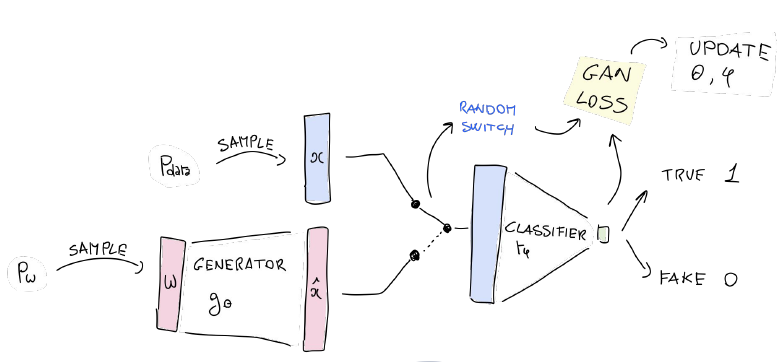
\includegraphics[width=1\linewidth]{imgs/chapter12/img16}
		\caption{Training}
		\label{fig:chapter12-16}
	\end{minipage}%
	\begin{minipage}{.5\textwidth}
		\centering
		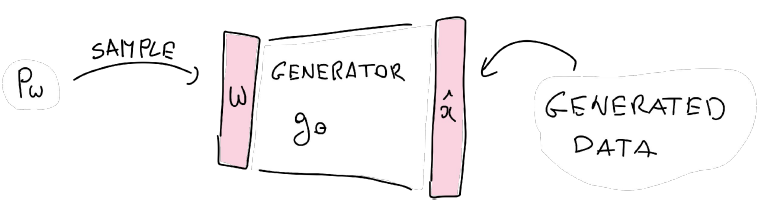
\includegraphics[width=1\linewidth]{imgs/chapter12/img17}
		\caption{Testing}
		\label{fig:chapter12-17}
	\end{minipage}
\end{figure}

\subsubsection{Ottimizzazione}
Il gradiente del obiettivo del GAN rispetto ai parametri del generatore $\theta$ $\frac{\partial}{\partial\theta}\max_\varphi V(\theta,\varphi)$ e richiede la risoluzione del problema di massimizzazione con rispetto al parametro del discriminatore $\varphi$.
Questo dovrebbe essere proibitivo computazionalmente.
In pratica si alterna uno step di update per il generatore dopo $k$ update per il discriminatore, senza garanzia di convergenza.

\paragraph{Esempio con vanilla SGD}
\begin{multicols}{2}
	\begin{itemize}
		\item Il discriminatore si aggiorna $k$ volte: $\varphi = \varphi + \nu\frac{\partial}{\partial\varphi}V(\theta,\varphi)$.
		\item Il generatore si aggiorna $\theta = \theta-\nu\frac{\partial}{\partial\theta}V(\theta,\varphi)$
	\end{itemize}
\end{multicols}
Le aspettative nei gradienti con rispetto a $p_{data}$ e a $p_\omega$ sono stimate su mini-batch.

\subsubsection{Problemi con GAN}
\begin{itemize}
	\item Training stability: i parametri oscillano e non convergono.
	\item Mode collapse: il generatore potrebbe imparare a perfezionare pochi esempi dal training set e riprodurre solo quegli esempi per vincere sempre.
	\item Vanishing gradient: se il discriminatore \`e molto bravo e lascia il generatore con poco gradiente per imparare.
\end{itemize}

\subsubsection{Altri tipi di GAN}
Diversi modelli simili a GAN possono essere costruiti considerando diverse divergenze tra le probabilit\`a e applicando trucchi simili per eliminare la necessit\`a di conoscere la densit\`a esplicitamente:
\begin{multicols}{2}
	\begin{itemize}
		\item \emph{f-GANS} costruite su f-divergenza.
		\item \emph{b-GANS} costruite su Bergman divergenza.
		\item \emph{Wasserstein GAN} utilizzano la Wasserstein metric.
		\item Altre GAN possono essere derivate utilizzando altre metriche integrali di probabilit\`a.
		\item \emph{f-GANS} su f-divergenza.
	\end{itemize}
\end{multicols}
GAN e VAE possono essere combinate e GAN condizionali esistono che lavorano simile a VAE continual.

	\chapter{Reinforcement learning}

\section{Introduzione}
L'idea del Reinforcement learning \`e che si ha un agente e un ambiente: l'agente svolge azioni che cambiano l'ambiente e conseguentemente l'ambiente ritorna all'agente delle rewards.
Questa idea viene presa dalle strategie di animali:
\begin{itemize}
	\item L'ambiente si trova in uno stato $s$.
	\item L'agente svolge un'azione.
	\item L'azione modifica l'ambiente.
	\item L'ambiente ritorna una reward all'agente e il nuovo stato $s'$.
\end{itemize}

	\subsection{Policy}
	L'agente tenta di imparare una policy o un mapping da stati a azioni in modo da massimizzare la reward data dall'ambiente.
	
	\section{Markov decision process (MDP)}
	MDP utilizza l'assuzione di Markov in cui uno stato al tempo $t$ dipende solo dallo stato precedente $s(t-1)$ e dall'azione precedente $a(t-1)$ per trovare una policy.
	Questo utilizza l'equazione di Bellman e la programmazione dinamica.
	L'obiettivo \`e trovare una policy, una mappa che ritorna tutte le azioni ottimali di ogni stato sul nostro ambiente.
	
	\subsection{Componenti}
	\begin{itemize}
		\item Stati $s_i$ che iniziano con uno stato $s_0$.
		\item Azioni $a$.
		\item Modello di transizione $P(s'|s,a)$, secondo l'assunzione di Markov la probabilit\`a di arrivare a $s'$ da $s$ dipende solo da $s$ e non da nessuna delle azioni passate o stati passati.
		\item Reward function $r(s)$.
		\item Policy $\pi(s)$, l'azione che un agente svolge in ogni stato dato.
	\end{itemize}
	Si nota come una MDP \`e definita dalla tupla $(S, A, R, P, y)$, dove $S$ \`e l'insieme degli stati possibili, $A$ l'insieme delle azioni possibili, $R$ la distribuzione delle reward dato uno stato, $P$ la probabilit\`a di transizione o la distribuzione rispetto al prossimo stato dato $(stato, azione)$ e $y$ il discount factor.
	La reward viene utilizzata per ottenere la policy migliore.
	L'obiettivo \`e pertanto di trovare la policy ottimale.
	
	\subsection{Ambienti stocastici}
	MDP viene utilizzata tipicamente negli ambienti stocastici, pertanto lo stato a tempo $t+1$ non \`e deterministico quando si conosce lo stato $s_t$ e l'azione $a_t:s_{t+1}$ viene estratta dalla probabilit\`a di transizione e deriva da un processo stocastico.
	
	\begin{figure}
		\centering
		\begin{minipage}{.5\textwidth}
			\centering
			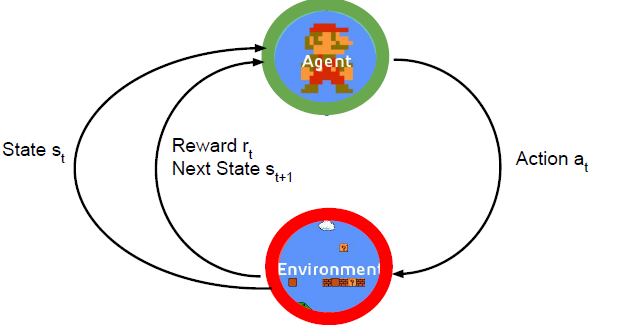
\includegraphics[width=0.7\linewidth]{imgs/chapter13/img0}
			\caption{Reinforcement learning}
			\label{fig:chapter13-00}
		\end{minipage}%
		\begin{minipage}{.5\textwidth}
			\centering
			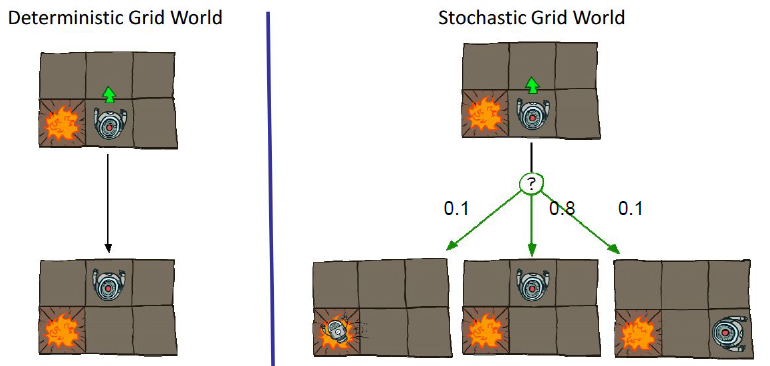
\includegraphics[width=1\linewidth]{imgs/chapter13/img1}
			\caption{Esempi di ambienti}
			\label{fig:chapter13-01}
		\end{minipage}
	\end{figure}
	
	\subsection{MDP loop}
	\begin{itemize}
		\item A tempo $t=0$ l'ambiente si campiona nello stato iniziale $s_0\sim p(s_0)$.
		\item Si ripete:
		\begin{itemize}
			\item L'agente seleziona l'azione $a_i$.
			\item L'ambiente campiona la reward $r_t\sim R(\cdot|s_t, a_t)$.
			\item L'ambiente campiona il prossimo stato $s_{t+1}\sim P(\cdot|s_t, a_t)$
			\item L'agente riceve la reward $r_t$ e lo stato successivo $s_{t+1}$.
		\end{itemize}
	\end{itemize}
	
	\subsection{Policy}
	La policy $\pi(s)$ \`e la funzione da $S$ ad $A$ che specifica quale azione prendere in ogni stato.
	Si deve trovare la policy $\pi^*$ che massimizza cumulative discounted rewards.
	La reward viene data dalla funzione
	$$R:(stato, azione)\rightarrow reward$$

		\subsubsection{Cumulative discounted reward}
		Si supponga di avere una policy $\pi$ in uno stato di inizio $s_0$ che porta a una sequenza $s_0,\dots, s_n$.
		La cumulative reward della sequenza \`e:
		$$\sum\limits_{t\ge 0} r(s_t)$$
		\`E pertanto la somma delle reward di una serie di stati.
		Quella discounted \`e una cumulative reward che d\`a un peso a diverse reward in base al tempo dello step:
		$$\sum\limits_{t\ge 0} y^tr(s_t)\qquad\ where\ 0 < y\le 1$$
		Il discount factor \`e un modo di pesare l'importanza dei primi passi o dei passi futuri in accordo con il valore di $y^t$.
		Minore \`e il discount factor \`e minore l'importanza di reward future e l'agente tende a concentrarsi su azioni che portano a reward immediate.
		Questa strategia aiuta gli algoritmi a convergere.

\section{Confronto tra reinforcement learning e supervised learning}

	\subsection{Supervised learning loop}
	\begin{itemize}
		\item Prendi input $x_i$ campionato dalla distribuzione dei dati.
		\item Utilizza un modello con parametri $w$ per predirre l'output $y$.
		\item Osserva l'output obiettivo $y_i$ e loss $l(w, x_i, y_i)$.
		\item Aggiorna $w$ per ridurre la loss con SGD: $w = w -\eta\nabla l(w, x_i, y_i)$.
	\end{itemize}
	
	\subsection{Reinforcement learning loop}
	\begin{itemize}
		\item Dallo stato $s_i$ svolgi un azione $a$ determinata dalla policy $\pi(s)$.
		\item L'ambiente seleziona lo stato successivo $s'$ in base al modello di transizione $P(s'|s,a)$.
		\item Osserva $s'$ e la reward $r(s)$, aggiornando la policy.
	\end{itemize}
	
	\subsection{Differenze fondamentali}
	\begin{itemize}
		\item Nel SL i dati non dipendono dall'input precedente, mentre in RL le azioni dell'agente influiscono il prossimo input.
		\item In SL si ha una loss function che guida il modello ai parametri migliori e si pu\`o differenziare con rispetto ai pesi, mentre in RL la reward guida lo sviluppo del modello, ma non \`e differenziabile rispetto ai paramatri.
		\item In SL si trova supervisione rispetto ad ogni passo, mentre in RL le rewards potrebbero essere sparse.
	\end{itemize}

\section{Metodi di reinforcement learning}
Per RL si trovano due approcci principali:
\begin{itemize}
	\item Metodi basati sul valore: una value function $V(s)$ viene introdotta e l'agente vuole masssimizzarla.
	La value di ogni stato \`e la quanit\`a totale di reward un agente pu\`o aspettarsi di collezionare rispetto al futuro cominciando da uno stato dato.
	\item Metodo basato sulla policy: si definisce una policy da ottimizzare direttamente, questa definisce come l'agente si comporta nella forma di distribuzione di probabilit\`a tra le azioni da svolgere in uno stato dato.
	Una policy stocastica d\`a la distribuzione di probabilit\`a su azioni diverse: $\pi_\theta(s,a)\approx P(a|s)$.
	
\end{itemize}

	\subsection{Value based methods}
	La funzione di value \`e una funzione dello stato con rispetto a una certa policy $\pi$.
	Ritorna la quantit\`a totale di reward che l'agente pu\`o aspettarsi da uno stato particolare a tutti gli stati possibili a partire da quello.
	Attraverso la value si pu\`o trovare una policy.
	La value function $V$ di uno stato con rispetto a una policy $\pi$ \`e l'aspettata cumulative reward di seguire tale policy cominciando in $s$:
	$$V^\pi(s) = \mathbb{E}\biggl[\sum\limits_{t\ge 0} y^tr(s_t)|s_0 = s,\pi\biggr]$$
	Con $a_t = \pi(s_t), s_{t+1}\sim P(\cdot|s_t, a_t)$.
	Il valore ottimale di uno stato \`e il valore raggiungibile seguendo la migliore policy:
	$$V^*(s) = \max_\pi\mathbb{E}\biggl[\sum\limits_{t\ge 0} y^tr(s_t)|s_0 = s,\pi\biggr]$$
	Dice pertanto quanto \`e buono uno stato.
	Si trova il valore atteso in quanto la sequenza di stati non \`e deterministica e non si ha accesso alla probabilit\`a di transizione.
	Rappresenta il valore che l'agente pu\`o aspettarsi da tutti gli stati possibili cominciando dallo stato iniziale $s$.

		\subsubsection{Q value function}
		Invece di gestire con la value function si utilizza la $Q$-value function che lavora con uno stato $s$, una azione $a$ e una policy $\pi$.
		Viene definita come:
		$$Q^\pi(s,a) = \mathbb{E}\biggl[\sum\limits_{t\ge 0} y^tr(s_t)|s_0 = s,a_0 = a\pi\biggr]$$
		Il valore ottimale di $Q$ dice quando \`e buona una coppia stato azione:
		$$Q^*(s,a) =\max_\pi\mathbb{E}\biggl[\sum\limits_{t\ge 0} y^tr(s_t)|s_0 = s,a_0 = a\pi\biggr]$$
		La Q value ottimale viene usata per computare la policy ottimale:
		$$\pi^*(s) = arg\max_aQ^*(s,a)$$
		La formula risultate della $Q$ value function \`e nella formula di un'equazione di Bellman:
		\begin{align*}
			Q^*(s,a) &= r(s) + y\sum\limits_{s'}P(s'|s,a)\max_{a'}Q^*(s',a')\\
			&=\mathbb{E}_{s'\sim P(\cdot|s,a)}[r(s)+y\max_{a'}Q^*(s',a')|s,a]
		\end{align*}
		Se il valore ottimale della coppia stato azione per il prossimo passo $Q^*(s',a')$ sono conosciuti allora la strategia ottima \`e svolgere l'azione che massimizza il valore atteso.
		Per calcolare il valore $Q$ dello stato corrente si deve calcolare il valore $Q$ degli stati vicini e cos\`i via con ricorsione.
		
		\subsubsection{Algoritmo Q-learning}
		Lo scopo di questo algoritmo \`e che la matrice di value $R$ \`e conosciuta unicamente all'ambiente e l'agente deve impararla con l'esperienza.
		L'agente possiede una matrice $Q$ che codifica stato, azione e rewards, ma \`e inizializzata a $0$ e diventa $R$ attraverso l'esperienza.
		La policy si ottiene attraverso questa matrice.
		\begin{enumerate}
			\item Inizializza la matrice $Q$ con zero.
			\item Seleziona uno stato iniziale casuale.
			\item Per ogni episodio (insieme di azioni che parte dallo stato iniziale e arriva allo stato finale).
			\item Mentre lo stato non \`e lo stato obiettivo.
			\item Seleziona una possibile azione casuale per lo stato corrente.
			\item Utilizzando l'azione considera arrivare allo stato prossimo.
			\item Ottieni il valore di $Q$ massimo per il prossimo stato.
			\item $Q^*(s,a) = R(s,a)+y\max\limits_a[Q^*(s',a')]$.
		\end{enumerate}
		Per trovare la policy ottimale:
		\begin{enumerate}
			\item Si pone lo stato corrente a quello iniziale.
			\item Dallo stato corrente si trova l'azione con il maggiore $Q$ value.
			\item Si pone lo stato corrente al prossimo.
			\item Si ripetono i passi $2$ e $3$ fino a che si raggiunge lo stato obiettivo.
		\end{enumerate}

		\subsubsection{Deep Q learning}
		L'equazione di Bellman pu\`o pertanto essere usate per imparare tabelle $Q$ per ritornare la policy ottimale.
		Nel mondo reale per\`o gli stati e le rewards possono essere troppo grandi per essere calcolate completamente.
		Per questa ragione viene introdotto un algoritmo di deep $Q$ learning che sfrutta l'idea di approssimare $Q$ utilizzando una funzione parametrica trainata da una NN.
		Si pu\`o approssimare $Q$ a
		$$Q^*(s,a) \approx Q_w(s,a)$$
		In quanto $Q_w$ \`e una funzione dei pesi $w$ si pu\`o trainare una NN per approssimare $Q_w$.
		Ad ogni interazione del training si aggiornano i parametri $w$ del modello per avvicinare $Q$ a $y$:
		$$y_i(s,a) = \mathbb{E}_{s'\sim P(\cdot|s,a)}[r(s)+y\max_{a'}Q_{w_{i-1}}(s',a')|s,a]$$
		La loss function
		$$L_i(w_i) = \mathbb{E}_{s,a\sim \rho}[(y_i(s,a) - Q_{w_i}(s,a))^2]$$
		Dove $\rho$ \`e la distribuzione di probabilit\`a sugli stati $s$ e le azioni $a$ che si riferiscono come distribuzione di comportamento.
		Si definisce a ogni iterazione $i$ e un target $y_i$ ottenuti attraverso la Bellman equation.
		Dati questi valori si pu\`o derivare $L_i$.
		Aggiornamento del gradiente:
		\begin{align*}
			\nabla_{w_i}L(w_i) &= \mathbb{E}_{s,a\sim\rho}[(y_i(s,a) - Q_{w_i}(s,a))\nabla_{w_i}Q_{w_i}(s,a)]=\\
			&= \mathbb{E}_{s,a\sim\rho,s'}[(r(s) + y\max_{a'}Q_{w_{i-1}}(s',a')-Q_{w_i}(s,a))\nabla_{w_i}Q_{w_i}(s,a)]
		\end{align*}
		Attraverso il training SGD si sostituisce il valore atteso campionando l'esperienza $(s,a,s')$ utilizzando la distribuzione di comportamento e il modello di transizione.
		
		\paragraph{Problematiche}
		Il training \`e prono all'instabilit\`a e a differenza del supervised learning i target si muovono.
		Esperienze successive sono correlate e dipendenti dalla policy che pu\`o cambiare rapidamente con piccoli cambi nei parametri, portando a un cambio drastico nella distribuzione dei dati.
		Per risolverli si pu\`o fare freezing sulla target Q network per aumentare la stabilit\`a della rete e utilizzare un experience replay: un buffer per salvare esperienze e campionare da quello in modo da seguire una strategia greedy che permette un trade-off tra exploitation ed esploration.

	\subsection{Policy gradient methods PGM}
	L'obiettivo dei PGM \`e di definire parametri che influenzano la policy $\pi$ e di impararli direttamente.
	Questa \`e la soluzione pi\`u semplice nel caso in cui si abbia uno spazio degli stati grande e continuo.
	L'idea \`e di utilizzare deep neural network per imparare la policy.
	Si deve pertanto imparare una funzione che ritorna la distribuzione di probabilit\`a di azioni rispetto allo stato corrente:
	$$\pi_\theta(s,a)\approx P(a|s)$$
	Si noti come questa ha un significato diverso rispetto ai value-based method: \`e una probabilit\`a di azioni rispetto agli stati, non una funzione da azioni a stati.
	In questo caso non si hanno le labels in modo da dare feedback alla NN attraverso backpropagation e viene usata la reward.
	Si devono pertanto trovare i migliori parametri $\theta$ della policy per massimizzare la reward aspettata attraverso gradient descent:
	\begin{align*}
		J(\theta) &= \mathbb{E}\biggl[\sum\limits_{t\ge 0}y^tr_t|\pi_\theta\biggr]\\
		&=\mathbb{E}_\tau[r(t)]
	\end{align*}
	Si vuole il valore atteso di ritorno di traiettorie: $\tau(s_0,a_0,r_0, \dots, s_n,a_n,r_n)$
	$$J(\theta) = \int_\tau r(\tau)p(\tau,\theta)d\tau$$
	Dove $p(\tau,\theta)$ \`e la probabilit\`a della traiettoria $\tau$ sotto la policy con i parametri $\theta$:
	$$p(\tau,\theta) = \prod\limits_{t\ge 0}\pi_\theta(s_t,a_t)P(s_{t+1}|s_t,a_t)$$
	Le traiettorie sono una semplificazione, un oggetto che rappresenta stato, azione e reward.
	In quanto l'integrale \`e di difficile risoluzione si differenzia utilizzando la log-trasformation:
	$$\nabla_\theta J(\theta) =\mathbb{E}_\tau[r(t)\nabla_\theta\log p(\tau,\theta)]$$
	Dove
	$$\log p(\tau,\theta) = \sum\limits_{t\ge 0} [\log \pi_\theta(s_t,a_t) + \log P(s_{t+1}|s_t,a_t)]$$
	E
	$$\nabla_\theta \log p(\tau,\theta) = \sum\limits_{t\ge 0}\nabla_\theta \log\pi_\theta(s_t,a_t)$$
	In questo modo si pu\`o computare il gradiente senza conoscere la probabilit\`a di transizione $p$.
	$$\nabla_\theta J(\theta) = \mathbb{E}_\tau\biggl[\biggl(\sum\limits_{t\ge 0}y^tr_t\biggr)\biggl(\sum\limits_{t\ge 0}\nabla_\theta\log\pi_\theta(s_t,a_t)\biggr)\biggr]$$
	Si pu\`o inoltre evitare di computare tutte le traiettorie possibili e usare unicametne un'approssimazione stocastica a $N$ traiettorie.
	$$\nabla_\theta J(\theta) \approx \dfrac{1}{N}\sum\limits_{i=1}^n\biggl(\sum\limits_{t = 0}^{T_i}y^tr_{i,t}\biggr)\biggl(\sum\limits_{t= 0}^{T_i}\nabla_\theta\log\pi_\theta(s_{i,t},a_{i,t})\biggr)$$

		\subsubsection{Reinforce}
		Reinforce \`e un algoritmo per deep RL che aggiorna i parametri:
		\begin{enumerate}
			\item Campiona $N$ traiettorie $\tau_i$ utilizzando la policy corrente $\pi_\theta$.
			\item Stima il gradiente di policy $\nabla_\theta J(\theta)$.
			\item Aggiorna i parametri attraverso gradient ascent $\theta = \theta + \eta\nabla_\theta J(\theta)$.
		\end{enumerate}
		
		\subsubsection{Single step reinforce}
		Single step reinforce \`e una variante del reinforce che stima il gradiente unicamente su uno step e non sull'intera traiettoria:
		\begin{enumerate}
			\item In uno stato $s$ campiona l'azione $a$ utilizzando la policy corrente $\pi_\theta$ e si osserva la reward $r$.
			\item Stima il gradiente $\nabla_\theta J(\theta)\sim r\nabla_\theta\log\pi_\theta(s,a)$
			\item Aggiorna i parametri attraverso gradient ascent $\theta = \theta + \eta\nabla_\theta J(\theta)$.
		\end{enumerate}
		Si nota come $r$ alto aumenta la probabilit\`a dell'azione vista, mentre se \`e basso si abbassa la probabilit\`a.
		Si aggiorna il parametri $\theta$ in accordo con il gradiente in quanto si vuole aumentare la reward o gradient ascent.


\end{document}
